\chapter{Compression Members}
Compression members include columns, truss members, braces, etc. Unlike tension members, their compressive strength is affected by multiple factors which are summarised below. They usually have more stocky sections than tension members to prevent premature strength loss due to buckling.
\begin{figure}[H]
\centering\footnotesize
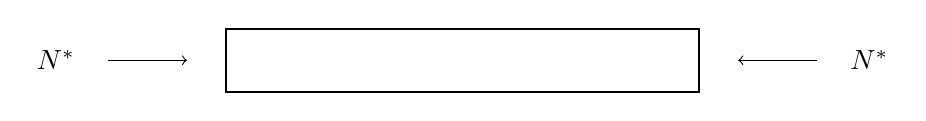
\begin{tikzpicture}
\draw[thick](0,-.4)rectangle(6,.4);
\draw[<-](6.5,0)--++(1,0)node[right=3mm]{$N^*$};
\draw[<-](-.5,0)--++(-1,0)node[left=3mm]{$N^*$};
\end{tikzpicture}
\end{figure}
\section{Factors Affecting Compressive Strength}
\subsection{Elastic Buckling}
Consider the elastic member buckling in axial compression below.
\begin{figure}[H]
\centering\footnotesize
\begin{subfigure}[b]{.49\linewidth}
\centering
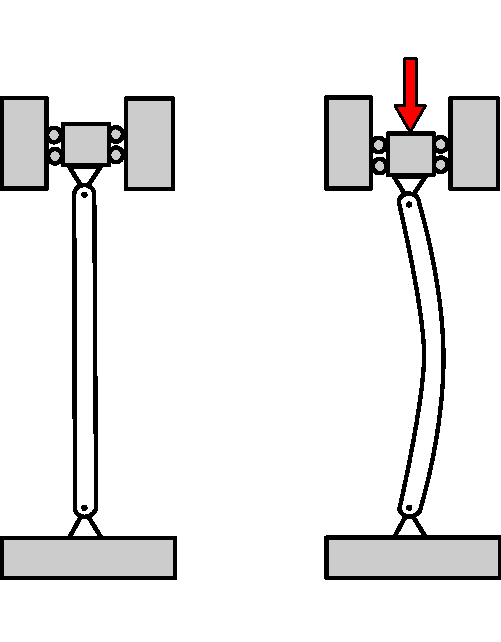
\includegraphics[height=6cm]{PIC/CH04/BUCKLING}
\end{subfigure}
\begin{subfigure}[b]{.49\linewidth}
\centering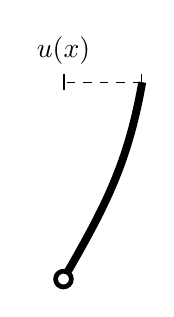
\begin{tikzpicture}
\CoorOrigin{0,0}[u][x]{1.5}
\HingeSupport{0,0}
\draw[dashed,|-|](1,2.5)--++(-1,0)node[fill=white,above=1mm]{$u(x)$};
\draw[line width=1mm](0,0)node[circle,inner sep=0,minimum size=2mm,fill=white,draw,line width=.6mm]{}to[out=60,in=-100](1,2.5);
\setstructmech{convention=direction}
\NodalForce{1,4.5}[N][-P][M]
\end{tikzpicture}
\end{subfigure}
\caption{Elastic buckling of a pinned--pinned column}
\end{figure}

From the free body diagram, the deflection $u(x)$ of an elastic column of length $L$ under axial load $P$ is related to the bending moment $M$ such that
\begin{gather*}
Pu=M\qquad\longrightarrow\qquad{}M=-EI\dfrac{\md{^2u}}{\md{x^2}}\qquad\longrightarrow\qquad{}EI\dfrac{\md{^2u}}{\md{x^2}}+Pu=0.
\end{gather*}
This is a homogeneous second order ODE. Techniques learnt in \textit{EMTH 210} and \textit{ENCN 304} can be applied to solve it subject to different boundary conditions. The general solution can be found as
\begin{gather*}
u(x)=A\cos\left(\eta{}x\right)+B\sin\left(\eta{}x\right)
\end{gather*}
where $\eta=\sqrt{\dfrac{P}{EI}}$ (the conventional $\lambda$ is retained to define other quantity), $A$ and $B$ are two constants.

For pinned--pinned member, $u(0)=u(L)=0$, $\eta$ can be found as
\begin{gather*}
\eta=\dfrac{n\pi}{L}
\end{gather*}
with $n=0,1,2,3,\cdots$. Thus,
\begin{gather*}
P_n=\dfrac{n^2\pi^2EI}{L^2}.
\end{gather*}
\begin{figure}[H]
\centering
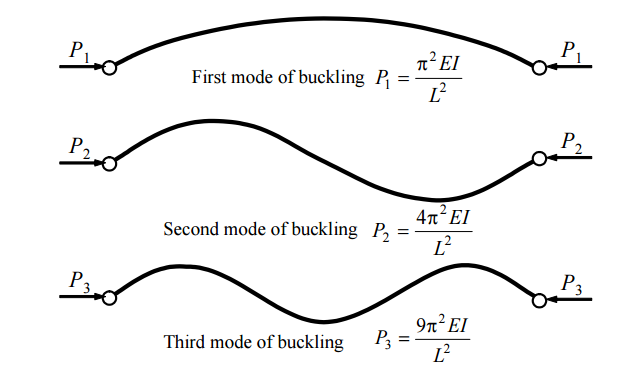
\includegraphics[width=12cm]{PIC/CH04/BMODE}
\caption{First three modes of buckling loads (\href{https://en.wikipedia.org/wiki/Euler\%27s_critical_load}{\url{https://en.wikipedia.org/wiki/Euler\%27s_critical_load}})}
\end{figure}

For non-trivial solution, the buckling load $P_{cr}$ would be the lowest possible load, which is
\begin{gather*}
P_{cr}=P_1=\dfrac{\pi^2EI}{L^2}.
\end{gather*}
For other boundary conditions, similar procedures can be carried out.

In general, the buckling strength $N_{om}$ of a column is expressed as
\begin{gather*}
N_{om}=P_{cr}=\dfrac{\pi^2EI}{\left(k_eL\right)^2}=\dfrac{\pi^2EI}{L_e^2},
\end{gather*}
where $k_e$ is the effective length factor with can be obtained by the above procedure for different boundary conditions, $L_e=k_eL$ is known as the effective length. It is the distance between buckling points of inflection for a flexural member. The following are a few examples.
\begin{figure}[H]
\footnotesize\centering
\begin{tikzpicture}
\FixedSupport{0,0}
\FixedSupport[180]{0,4}
\FixedSupport{5,0}
\HingeSupport[180]{5,4}
\HingeSupport[180]{10,4}
\HingeSupport{10,0}
\draw[very thick](0,0)to[out=90,in=-90]node(A)[pos=0.5,circle,fill=red,inner sep=0,minimum size=2mm]{}(.4,2);
\draw[very thick](0,4)to[out=-90,in=90]node(B)[pos=0.5,circle,fill=red,inner sep=0,minimum size=2mm]{}(.4,2);
\draw[very thick](5,0)to[out=90,in=-60]node(C)[pos=0.3,circle,fill=red,inner sep=0,minimum size=2mm]{}(5,4)node[joint]{};
\draw[very thick](10,0)node[joint]{}to[out=70,in=-70](10,4)node[joint]{};
\draw[|<->|](-1,1)--++(0,2)node[midway,fill=white]{$L_e=0.5L$};
\draw[|<->|](4,4)--++(0,-2.8)node[midway,fill=white]{$L_e=0.7L$};
\draw[|<->|](9,0)--++(0,4)node[midway,fill=white]{$L_e=L$};
\end{tikzpicture}\caption{Illustration of effective length}
\end{figure}

Dividing $N_{om}$ by cross section area, we define buckling stress $f_{om}$ as
\begin{gather*}
f_{om}=\dfrac{N_{om}}{A}=\underbrace{E}_\text{material}\cdot\underbrace{\dfrac{I}{A}}_\text{section}\cdot\underbrace{\dfrac{\pi^2}{\left(k_eL\right)^2}}_\text{length}.
\end{gather*}
Noting that the radius of gyration $r$ is defined as $r=\sqrt{I/A}$, then
\begin{gather*}
f_{om}=\dfrac{\pi^2E}{\left(k_eL/r\right)^2}.
\end{gather*}
Given elastic modulus $E$ is a constant, $f_{om}$ is essentially a function of $k_eL/r$, we define the slenderness ratio $\lambda$ as
\begin{gather*}
\lambda=\dfrac{k_eL}{r},
\end{gather*}
so that
\begin{gather*}
f_{om}=\dfrac{\pi^2E}{\lambda^2}.
\end{gather*}
\begin{exmp}Theoretical Buckling

Find the theoretical buckling load of a column with bottom end fixed and top end pinned. The length of column is $L$. The flexural rigidity is $EI$.
\begin{figure}[H]
\footnotesize
\begin{tikzpicture}
\FixedSupport{0,0}
\RollerSupport[-90]{0,3}
\draw[line width=1.2mm](0,0)to[out=90,in=-60](0,3);
\node[joint,fill=exmpbg]at(0,3){};
\draw[|->](-1,3)--++(0,-1)node[below]{$x$};
\end{tikzpicture}
\end{figure}
\end{exmp}
\begin{solution}
The problem is equivalent to find the particular solution for the ODE
\begin{gather*}
EI\dfrac{\md{^2u}}{\md{x^2}}+Pu=0.
\end{gather*}
subjected to boundary conditions
\begin{align*}
u(0)&=0,\qquad\longrightarrow\qquad\text{displacement is zero at top,}\\
u(L)&=0,\qquad\longrightarrow\qquad\text{displacement is zero at bottom,}\\
\dfrac{\md{^2u}}{\md{x^2}}(0)&=0,\qquad\longrightarrow\qquad\text{moment is zero at top,}\\
\dfrac{\md{u}}{\md{x}}(L)&=0,\qquad\longrightarrow\qquad\text{rotation is zero at bottom}.
\end{align*}
The critical load $P$ is the smallest value of the solved solution.

Since in this particular problem, second order derivative appears in BC, more advanced techniques (casting to a fourth order ODE) are needed to find the general solution, which can eventually be expressed as
\begin{gather*}
u(x)=A\cos\left(\eta{}x\right)+B\sin\left(\eta{}x\right)+Cx+D.
\end{gather*}
Using $u(0)=0$ and $\dfrac{\md{^2u}}{\md{x^2}}(0)=0$,
\begin{gather*}
u(0)=A+D=0,\qquad\longrightarrow\qquad{}A=-D,\\
\dfrac{\md{^2u}}{\md{x^2}}(0)=-A\eta^2=0,\qquad\longrightarrow\qquad{}A=D=0.
\end{gather*}
Since $\eta\neq0$ for non-trivial solution. The general solution after apply two BCs can be expressed as
\begin{gather*}
u(x)=B\sin\left(\eta{}x\right)+Cx.
\end{gather*}
Now apply $\dfrac{\md{u}}{\md{x}}(L)=0$,
\begin{gather*}
\dfrac{\md{u}}{\md{x}}(L)=B\eta\cos\left(\eta{}L\right)+C=0,\qquad\longrightarrow\qquad{}C=-B\eta\cos\left(\eta{}L\right).
\end{gather*}
Apply the last BC,
\begin{gather*}
u(L)=B\sin\left(\eta{}L\right)+CL=0,\qquad\longrightarrow\qquad{}B\left(\sin\left(\eta{}L\right)-\eta{}L\cos\left(\eta{}L\right)\right)=0.
\end{gather*}
In order to solve for non-trivial solution, $B$ cannot be zero otherwise all $A$, $B$, $C$ and $D$ would be zeros, leads to trivial solution. Thus,
\begin{gather*}
\sin\left(\eta{}L\right)-\eta{}L\cos\left(\eta{}L\right)=0,\qquad\longrightarrow\qquad{}
\tan\left(\eta{}L\right)=\eta{}L.
\end{gather*}
This is a transcendental equation. The approximate solution can be found via numerical, analytical approximations, or graphical methods.
\begin{figure}[H]
\centering\begin{tikzpicture}[domain=0:10][x=2cm]
\draw[thick,->](0,0)--(10,0)node[right]{$\eta{}L$};
\draw[thick,->](0,0)--(0,5);
\foreach\x in{.5,1.5,2.5}\draw[dashed, thick,red](\x*pi,-1)--++(0,6);
\draw[ultra thick,color=cc0066]plot[domain=0:.438*pi](\x,{tan(\x r)});
\foreach\x in{.5,1.5}\draw[ultra thick,color=cc0066]plot[domain=(\x+.25)*pi:(\x+.938)*pi] (\x,{tan(\x r)});
\draw[ultra thick,color=0066cc]plot[domain=0:5](\x,\x);
\node[below right]at(0,0){$0$};
\node[below right]at(pi/2,0){$\frac{\pi}{2}$};
\node[below right]at(pi,0){$\pi$};
\node[below right]at(3*pi/2,0){$\frac{3\pi}{2}$};
\node[below right]at(2*pi,0){$2\pi$};
\node[below right]at(5*pi/2,0){$\frac{5\pi}{2}$};
\node[circle,fill=red]at(4.49340945790906,4.49340945790906){};
\end{tikzpicture}
\end{figure}
The first non-trivial solution is $\eta{}L\approx4.4934$. This gives
\begin{gather*}
P_{cr}=\dfrac{4.4934^2EI}{L^2}=\dfrac{\pi^2EI}{\left(0.699L\right)^2},\qquad\longrightarrow\qquad{}k_e=0.699.
\end{gather*}

For this case, $k_e$ is often taken as \num{0.7}.
\end{solution}

For elastic material, the critical stress $f_{cr}$ is simply $f_{om}$, which approaches infinity when $\lambda$ approaches zero (i.e., very short columns). If one plots $f_{cr}$ with regard to $\lambda$, the following graph can be obtained.
\begin{figure}[H]
\centering\footnotesize
\begin{tikzpicture}[>=latex]
\begin{axis}[
width=10cm,
height=7cm,
xtick=\empty,
ytick=\empty,
axis x line=center,
axis y line=center,
xlabel={$\lambda$},
ylabel={$f$},
xlabel style={right},
ylabel style={left},
xmin=0,xmax=4.5,ymin=0,ymax=2]
\addplot[name path=B,samples=40,line width=1mm,color=black,mark=none,domain=0:4]{1/x/x}node[color=cc0066,above,pos=1]{$f_{om}$};
\addplot[name path=C,domain=0:4]{0};
\addplot[00cc66,opacity=.3]fill between[of=B and C];
\node[align=center]at(.5,.7){safe\\region};
\end{axis}
\end{tikzpicture}
\caption{Theoretical governing region for $f_{cr}$ for elastic material}
\end{figure}
\subsection{Compressive Strength}
However, for real life situations, no matter how small $\lambda$ is, a $f_{om}$ greater than yield strength $f_y$ is meaningless. The yield strength $f_y$ is often considered as a material property that does not vary with $\lambda$. The critical stress $f_{cr}$ shall be the minimum of $f_y$ and $f_{om}$. If one draws $f_{cr}$ against $\lambda$, the following graph can be obtained. It affects short members.
\begin{figure}[H]
\centering\footnotesize
\begin{tikzpicture}[>=latex]
\begin{axis}[
width=10cm,
height=7cm,
xtick=\empty,
ytick=\empty,
axis x line=center,
axis y line=center,
xlabel={$\lambda$},
ylabel={$f$},
xlabel style={right},
ylabel style={left},
xmin=0,xmax=4.5,ymin=0,ymax=2]
\addplot[name path=A,line width=1mm,color=black,mark=none,domain=0:.8]{1.5625};
\addplot[name path=B,samples=40,line width=1mm,color=black,mark=none,domain=.8:4]{1/x/x}node[color=cc0066,above,pos=1]{$f_{om}$};
\addplot[dashed,very thick,color=0066cc,mark=none,domain=.8:1.5]{1.5625}node[above,pos=1]{$f_y$};
\addplot[dashed,samples=10,very thick,color=cc0066,mark=none,domain=0:.8]{1/x/x};
\addplot[name path=C,domain=0:.8]{0};
\addplot[name path=D,domain=.8:4]{0};
\addplot[00cc66,opacity=.3]fill between[of=A and C];
\addplot[00cc66,opacity=.3]fill between[of=B and D];
\node[align=center]at(.5,.7){safe\\region};
\end{axis}
\end{tikzpicture}
\caption{Theoretical governing region for $f_{cr}$}
\end{figure}
\subsection{Local Buckling}
Section can buckle under complex stress conditions. The buckling of web/flanges would further reduce section compression capacity. If often depends on flange/web slenderness ($b_f/t_f$ and $d/t_w$). It affects short members.
%\begin{figure}[H]
%\centering
%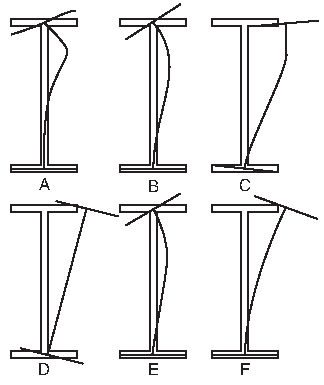
\includegraphics[width=8cm]{PIC/CH04/LB}
%\caption{Local buckling modes of I sections}
%\end{figure}
\begin{figure}[H]
\centering\footnotesize
\begin{tikzpicture}[>=latex]
\begin{axis}[
width=10cm,
height=7cm,
xtick=\empty,
ytick=\empty,
axis x line=center,
axis y line=center,
xlabel={$\lambda$},
ylabel={$f$},
xlabel style={right},
ylabel style={left},
xmin=0,xmax=4.5,ymin=0,ymax=1.7]
\addplot[dashed,line width=.4mm,color=black,mark=none,domain=0:.8]{1.5625};
\addplot[dashed,samples=40,line width=.4mm,color=black,mark=none,domain=.8:4]{1/x/x};
\addplot[name path=A,line width=1mm,color=black,mark=none,domain=0:.9]{1.234567901};
\addplot[name path=B,samples=40,line width=1mm,color=black,mark=none,domain=.9:4]{1/x/x};
\addplot[dashed,very thick,mark=none,domain=0:1.5]{1.234567901}node[right,pos=1,align=center]{reduced strength\\due to local buckling};
\addplot[name path=C,domain=0:.9]{0};
\addplot[name path=D,domain=.9:4]{0};
\addplot[00cc66,opacity=.3]fill between[of=A and C];
\addplot[00cc66,opacity=.3]fill between[of=B and D];
\node[align=center]at(.5,.6){safe\\region};
\end{axis}
\node[anchor=center]at(12,2.7){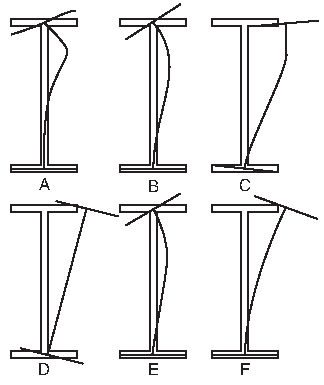
\includegraphics[height=6cm]{PIC/CH04/LB}};
\end{tikzpicture}
\caption{Governing region considering local buckling}
\end{figure}
\subsection{Residual Stress}
All members contain residual stresses due to uneven cooling. These result in earlier yielding
and a reduction in elastic modulus.

Due to residual stresses, the tangent stiffness $E_T$ decreases gradually so that $E_T<E$. Recall $f_{om}=\dfrac{\pi^2E}{\lambda^2}$, when $E$ decreases, $f_{om}$ would decease accordingly as $\dfrac{\pi^2E_T}{\lambda^2}<\dfrac{\pi^2E}{\lambda^2}$.
\begin{figure}[H]
\centering\footnotesize
\begin{tikzpicture}[>=latex]
\begin{axis}[
width=10cm,
height=5.5cm,
xtick=\empty,
ytick=\empty,
axis x line=center,
axis y line=center,
xlabel={strain},
ylabel={stress},
xlabel style={right},
ylabel style={left},
xmin=0,xmax=4.5,ymin=0,ymax=2]
\addplot[line width=.8mm,mark=none]coordinates{
(0,0)
(.3,1.5)
(3.5,1.5)
}node[align=left,above,pos=1]{ideal response\\without residual stress};
\addplot[line width=.8mm,color=cc0066,domain=0:3.5,samples=100]{1.5*(x/.3/(1+(x/.3)^2)^0.5)}node[align=left,below,pos=1]{response with\\residual stress};
\draw[<-](axis cs:.3,1)--++(.5,-.5)--++(.5,0)node[right]{$E$ decreases gradually};
\end{axis}
\end{tikzpicture}
\caption{Stress--strain curve considering residual stress}
\end{figure}
The effect is most significant on members of moderate slenderness, where the strength is reduced.
\begin{figure}[H]
\centering\footnotesize
\begin{tikzpicture}[>=latex]
\begin{axis}[
width=10cm,
height=6cm,
xtick=\empty,
ytick=\empty,
axis x line=center,
axis y line=center,
xlabel={$\lambda$},
ylabel={$f$},
xlabel style={right},
ylabel style={left},
xmin=0,xmax=4.5,ymin=0,ymax=1.7]
\addplot[dashed,line width=.4mm,color=black,mark=none,domain=0:.8]{1.5625};
\addplot[dashed,samples=40,line width=.4mm,color=black,mark=none,domain=.8:4]{1/x/x};
\addplot[name path=A,line width=1mm,color=black,mark=none,domain=0:.4]{1.234567901};
\addplot[name path=C,samples=40,line width=1mm,color=black,mark=none,domain=1.2:4]{1/x/x};
\addplot[dashed,very thick,mark=none,domain=0:1.5]{1.234567901}node[right,pos=1,align=center]{reduced strength\\due to local buckling};
\draw[name path=B,line width=1mm](.4,1.234567901)to[out=0,in=125.3594196](1.2,.6944);
\addplot[name path=D,domain=0:.4]{0};
\addplot[name path=E,domain=.4:1.2]{0};
\addplot[name path=F,domain=1.2:4]{0};
\addplot[cc0066,opacity=.3]fill between[of=A and D];
\addplot[00cc66,opacity=.3]fill between[of=B and E];
\addplot[0066cc,opacity=.3]fill between[of=C and F];
\node[rotate=90,anchor=west]at(axis cs:.2,.02){stocky};
\node[rotate=90,anchor=west]at(axis cs:.8,.02){moderate};
\node[rotate=90,anchor=west]at(axis cs:1.4,.02){slender};
\end{axis}
\end{tikzpicture}
\caption{Governing region considering residual stress}
\end{figure}
\subsection{Initial Out-of-Straightness and Eccentrical Loading}
An eccentricity $e=L/1500$ is commonly assumed. This is less than the maximum out-of-straightness camber of $L/1000$. The eccentricity introduces non-zero section moment ever if the member is axially loaded. This additional moment would lower theoretical critical buckling force.For straight members, the loading behaviour follows $O\rightarrow{}A\rightarrow{}B$ but the actual behaviour due to eccentricity is the dashed line.

\begin{figure}[H]
\centering
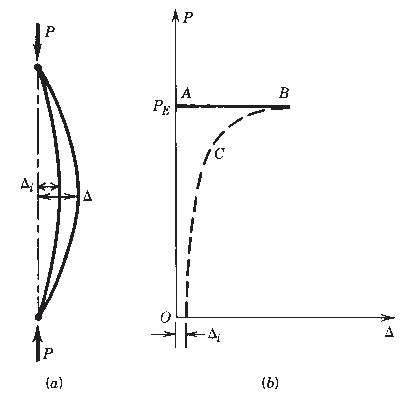
\includegraphics{PIC/CH04/OOS}
\caption{Effect of initial out-of-straightness on column behaviour}
\end{figure}
\begin{figure}[H]
\centering
\footnotesize
\begin{tikzpicture}
\draw[thick](0,-.8)rectangle(6,.8);
\draw[dashed](-1,0)--(7,0);
\draw[<-](6.5,.4)--++(1,0)node[right=3mm]{$N^*$};
\draw[<-](-.5,.4)--++(-1,0)node[left=3mm]{$N^*$};
\end{tikzpicture}
\caption{Eccentrical loading}
\end{figure}
The eccentrical loading has a similar effect to out-of-straightness and thus can be taken into account in a similar way. Both out-of-straightness and eccentrical loading affect slender members in a similar way.
\begin{figure}[H]
\centering\footnotesize
\begin{tikzpicture}[>=latex]
\begin{axis}[
width=10cm,
height=6cm,
xtick=\empty,
ytick=\empty,
axis x line=center,
axis y line=center,
xlabel={$\lambda$},
ylabel={$f$},
xlabel style={right},
ylabel style={left},
xmin=0,xmax=4.5,ymin=0,ymax=1.7]
\addplot[dashed,line width=.4mm,color=black,mark=none,domain=0:.8]{1.5625};
\addplot[dashed,samples=40,line width=.4mm,color=black,mark=none,domain=.8:4]{1/x/x};
\addplot[name path=A,line width=1mm,color=black,mark=none,domain=0:.4]{1.234567901};
\draw[name path=B,line width=1mm](.4,1.234567901)to[out=0,in=125.3594196](1.2,.8*.6944);
\addplot[name path=C,samples=40,line width=1mm,color=black,mark=none,domain=1.2:4]{.8/x/x*(6.8-x)/5.6};
\addplot[dashed,very thick,mark=none,domain=0:1.5]{1.234567901};
\addplot[name path=D,domain=0:.4]{0};
\addplot[name path=E,domain=.4:1.2]{0};
\addplot[name path=F,domain=1.2:4]{0};
\addplot[00cc66,opacity=.3]fill between[of=A and D];
\addplot[00cc66,opacity=.3]fill between[of=B and E];
\addplot[00cc66,opacity=.3]fill between[of=C and F];
\node[align=center]at(.5,.6){safe\\region};
\end{axis}
\end{tikzpicture}
\caption{Governing region considering initial OOS and eccentric loading}
\end{figure}
\section{Strength Design Concept}
The LRFD equation for columns has a similar form \NZSSTEEL{\S~6.1} to that of tension members.
\begin{gather}
N^*\leqslant\phi{}N_c=\phi{}\alpha_cN_s,
\end{gather}
where
\begin{conditions}
\phi&strength reduction factor, \num{0.9}\\
N_s&nominal section capacity\\
N_c&nominal member capacity
\end{conditions}
The design member strength $\phi{}N_c$ requires calculation of the section capacity $N_s$, and the member slenderness factor $\alpha_c$.
\subsection{Section Capacity}
The nominal section capacity $N_s$ is determined as:
\begin{gather}
N_s=k_fA_nf_y,
\end{gather}
where
\begin{conditions}
k_f&form factor\\
A_n&net area\\
f_y&yield stress
\end{conditions}

The form factor $k_f$ accounts for local buckling. It is defined to be the ratio between the effective area $A_e$ and gross area $A_g$.
\begin{gather*}
k_f=\dfrac{A_e}{A_g},
\end{gather*}
where $A_e=\sum{}b_{e,i}t_i$ and $b_{e,i}$ and $t_i$ are the effective width and thickness of each \textbf{individual} element. For a flat plate with thickness of $t$ and \textbf{clear} width of $b$ (outstand from the face of the supporting plate element,
or between the faces of the supporting plate elements), the effective width $b_e$ can be computed as
\begin{gather}
b_e=\min\left(b,~\lambda_{ey}t\sqrt{\dfrac{\SI{250}{\mpa}}{f_y}}\right),
\end{gather}
in which $\lambda_{ey}$ is the yield slenderness limit. For an I-section, values of $b_i$ and $t_i$ are shown below. There are 7 elements in total, 4 belong to flange which are one-edge supported while 1 belongs to web which is both-edge supported. Note the corresponding $b_{e,i}$ may be smaller than the physical length $b_i$.
\begin{figure}[H]
\centering\begin{tikzpicture}[x=1cm,y=1cm,scale=.5]
\draw[fill=0066cc](-.25,-4.5)rectangle(.25,4.5);
\draw[fill=cc0066](-2.5,-4.5)rectangle(2.5,-4);
\draw[fill=cc0066](-2.5,4)rectangle(2.5,4.5);
\draw[fill=00cc66](-.25,4)rectangle(.25,4.5);
\draw[fill=00cc66](-.25,-4)rectangle(.25,-4.5);
\draw[|<->|](3,-4)--++(0,8)node[midway,fill=white]{$b_5$};
\draw[|<->|](-.25,-5)--++(.5,0)node[midway,fill=white,below=3mm]{$t_5$};
\draw[|<->|](-2.5,5.5)--++(2.25,0)node[midway,fill=white]{$b_1$};
\draw[|<->|](2.5,5.5)--++(-2.25,0)node[midway,fill=white]{$b_2$};
\draw[|<->|](-2.5,-5.5)--++(2.25,0)node[midway,fill=white]{$b_3$};
\draw[|<->|](2.5,-5.5)--++(-2.25,0)node[midway,fill=white]{$b_4$};
\draw[|<->|](3,4)--++(0,.5)node[midway,fill=white,right=3mm]{$t_1,t_2$};
\draw[|<->|](3,-4)--++(0,-.5)node[midway,fill=white,right=3mm]{$t_3,t_4$};
\end{tikzpicture}
\caption{Five flat elements in a typical I section}
\end{figure}

If the slenderness for any element, $\lambda_{e,i}$, exceeds the yield limit $\lambda_{ey,i}$, the excess width is neglected when calculated the effective width $b_{e,i}$ for that element. Some universal beam sections have $k_f$ values slightly less than one. For flat plates, \NZSSTEEL{Table 6.2.4} gives the following limits shown in \figref{fig:flat_slenderness}.


An element, which has the same slenderness as the yield limit $\lambda_{ey}$, should just reach the yield stress before local buckling occurs. Elements which have higher levels of residual stresses from rolling and welding will reach the yield stress earlier and therefore have lower values of $\lambda_{ey}$.

The allowable slenderness of stiffened elements is much greater than that for unstiffened elements.
\begin{figure}[H]
\centering
\footnotesize\begin{tikzpicture}
\node at(0,1){
\begin{tabular}{llc}
	\toprule
	longitudinal edges supported & residual stresses & $\lambda_{ey}$ \\ \midrule
	\multirow{4}{*}{one}         & SR                &       16       \\
	                             & HR                &       16       \\
	                             & LW, CF            &       15       \\
	                             & HW                &       14       \\ \midrule
	\multirow{4}{*}{both}        & SR                &       45       \\
	                             & HR                &       45       \\
	                             & LW, CF            &       40       \\
	                             & HW                &       35       \\ \bottomrule
	\multicolumn{3}{l}{SR --- stress relived}                         \\
	\multicolumn{3}{l}{HR --- hot-rolled}                             \\
	\multicolumn{3}{l}{CF --- cold-formed}                            \\
	\multicolumn{3}{l}{LW --- lightly welded longitudinally}          \\
	\multicolumn{3}{l}{HW --- heavily welded longitudinally}          \\ \bottomrule
\end{tabular}
};
\node[align=left]at(8,2.5){The following illustrations show \textcolor{cc0066}{one} and \textcolor{0066cc}{both}\\edges supported for common sections.};
\draw[color=0066cc,line width=1.2mm](5.8,0)--++(0,1.5)node[midway,right=2mm]{S};
\draw[color=cc0066,line width=1.2mm](5,1.5)node[above]{U}--++(1.6,0)node[above]{U}(5,0)node[below]{U}--++(1.6,0)node[below]{U};
\draw[color=0066cc,line width=1.2mm](7.5,0)rectangle(9,1)node[midway]{S};
\draw[color=cc0066,line width=1.2mm](10,1.5)node[above]{U}--++(.8,0)--++(0,-1.5)--++(-.8,0)node[above]{U};
\draw[color=0066cc,line width=1.2mm](10.8,0)--++(0,1.5)node[midway,right]{U};
\draw[color=cc0066,line width=1.2mm](10,-2.5)node[right]{U}--++(0,1.5)node[right]{U}(10,-1.75)--++(.8,0)node[above]{U};
\draw[color=cc0066,line width=1.2mm](7.5,-1)node[right]{U}--++(0,-1)--++(1,0)node[above]{U};
\FixedSupport[-90]{5,4.5}
\FixedSupport[90]{7.5,4.5}
\draw[line width=1.2mm](5,4.5)--++(2.5,0)node[midway,below=5mm,align=center]{both edges supported\\stiffened, S};
\draw[line width=1.2mm,dashed](5,4.5)to[out=0,in=180](6.25,4.8)to[out=0,in=180](7.5,4.5);
\FixedSupport[-90]{8.5,4.5}
\draw[line width=1.2mm](8.5,4.5)--++(2.5,0)node[midway,below=5mm,align=center]{one edge supported\\unstiffened, U};
\draw[line width=1.2mm,dashed](8.5,4.5)to[out=0,in=210](11,5);
\end{tikzpicture}
\caption{Yield slenderness limits of flat plate elements}\label{fig:flat_slenderness}
\end{figure}

Often $k_f$ is provided with section parameters in the product specification manual.

\begin{exmp}
Assume Grade 300 steel, find the section capacity $N_s$ of a 310UB32.0 section.
\end{exmp}
\begin{solution}
\begin{minipage}{5cm}\centering\begin{tikzpicture}[x=1cm,y=1cm,scale=.5]
\draw[fill=0066cc](-.25,-4.5)rectangle(.25,4.5);
\draw[fill=cc0066](-2.5,-4.5)rectangle(2.5,-4);
\draw[fill=cc0066](-2.5,4)rectangle(2.5,4.5);
\draw[|<->|](3,-4)--++(0,8)node[midway,fill=exmpbg]{$d_1=282$};
\draw[|<->|](3,4)--++(0,.5)node[midway,fill=exmpbg,right=3mm]{$t_f=8$};
\draw[|<->|](-.25,-5)--++(.5,0)node[midway,fill=exmpbg,below=3mm]{$t_w=5.5$};
\draw[|<->|](-2.5,5.5)--++(5,0)node[midway,fill=exmpbg]{$b_f=149$};
\draw[fill=00cc66](-.25,4)rectangle(.25,4.5);
\draw[fill=00cc66](-.25,-4)rectangle(.25,-4.5);
\end{tikzpicture}
\end{minipage}
\begin{minipage}{.99\linewidth-5cm}
This is a hot-rolled section. The gross area is $A_g=\SI{4080}{\mm^2}$.

For flanges, only one side is supported. Thus, $\lambda_{ey,f}=16$.
\begin{gather*}
b_{e,f}=16\times\SI{8}{\mm}\times\sqrt{\dfrac{250}{320}}=\SI{113.14}{\mm}.
\end{gather*}
This is greater than the clear width $b=\dfrac{b_f-t_w}{2}=\SI{71.75}{\mm}$, hence $b_{e,f}=b=\SI{71.75}{\mm}$.

For web, both sides are supported. Thus, $\lambda_{ey,w}=45$.
\begin{gather*}
b_{e,w}=45\times\SI{5.5}{\mm}\times\sqrt{\dfrac{250}{320}}=\SI{218.76}{\mm}.
\end{gather*}
\end{minipage}

The effective area is then
\begin{gather*}
\begin{split}
A_e&=\sum{}b_{e,i}t_i=\underbrace{\SI{218.76}{\mm}\times\SI{5.5}{\mm}}_\text{web, blue}+\underbrace{4\times\SI{71.75}{\mm}\times\SI{8}{\mm}}_\text{flange, red}\\
&+\underbrace{2\times\SI{5.5}{\mm}\times\SI{8}{\mm}}_\text{connection, green}=\SI{3587.18}{\mm^2}.
\end{split}
\end{gather*}

The form factor $k_f=A_e/A_g=0.879$, which is smaller than the value listed (see the table in Liberty catalogue) of $0.915$. Since there is no area reduction, $A_n=A_g$.
\begin{gather*}
N_s=k_fA_gf_y=A_ef_y=\SI{3587.18}{\mm^2}\times\SI{320}{\mpa}=\SI{1147.9}{\kn}.
\end{gather*}
\end{solution}
\subsection{Member Capacity}\label{sec:n_c}
Before we introduce how to calculate \textbf{member} capacity, the concept of modified slenderness ratio $\lambda_n$ shall be discussed.

Since buckling plays a vital role in compression members, we can no more use the full length to compute slenderness ratio, instead, the effective length $L_e$ shall be used.
\begin{gather}
L_e=k_eL,
\end{gather}
where $k_e$ is the member effective length factor (\NZSSTEEL{Fig. 4.8.3.2}).

The modified slenderness ratio $\lambda_n$ is defined as
\begin{gather}
\lambda_n=\lambda\sqrt{k_f}\sqrt{\dfrac{f_y}{\SI{250}{\mpa}}}=\dfrac{L_e}{r}\sqrt{k_f}\sqrt{\dfrac{f_y}{\SI{250}{\mpa}}}.
\end{gather}
If $f_y=\SI{250}{\mpa}$ and $k_f=1$, then
\begin{gather*}
\lambda_n=\lambda=\dfrac{L_e}{r}.
\end{gather*}

The nominal member capacity $N_s$ is associated with the nominal section capacity $N_c$ via a reduction factor $\alpha_c$:
\begin{gather}
N_c=\alpha_cN_s,
\end{gather}
in which,
\begin{gather*}
\alpha_c=\xi\left(1-\sqrt{1-\left(\dfrac{90}{\xi\lambda'}\right)^2}\right),\qquad
\xi=\dfrac{\left(\dfrac{\lambda'}{90}\right)^2+1+\eta}{2\left(\dfrac{\lambda'}{90}\right)^2},
\end{gather*}
with
\begin{gather*}
\lambda'=\lambda_n+\alpha_a\alpha_b,\qquad
\eta=\max\left(0.00326\left(\lambda'-13.5\right),~0\right),\qquad
\alpha_a=\dfrac{2100\left(\lambda_n-13.5\right)}{\lambda_n^2-15.3\lambda_n+2050},
\end{gather*}
and $\alpha_b$ is the compression member section constant which are shown in \tabref{tab:alpha_b} that characterises sectional residual stress effects (also refer to \NZSSTEEL{Table 6.3.3(1)}).
\begin{table}[htbp]
\centering\footnotesize
\caption{Values of $\alpha_b$}\label{tab:alpha_b}
\begin{tabular}{m{10cm}cc}
	\toprule
	section type                                                                               &     $k_f$      & $\alpha_b$ \\ \midrule
	UB and UC sections, hot-rolled ($t_f\leqslant\SI{40}{\mm}$), Box sections, welded & $\leqslant1.0$ & \num{0.0}  \\
	UB and UC sections, hot-rolled ($t_f>\SI{40}{\mm}$)                               & $\leqslant1.0$ & \num{1.0}  \\
	RHS and CHS, hot-formed                                                                    &     $=1.0$     & \num{-1.0} \\
	RHS and CHS, cold-formed (stress relieved)                                                 &     $<1.0$     & \num{-0.5} \\
	RHS and CHS, cold-formed (non-stress relieved)                                             & $\leqslant1.0$ & \num{-0.5} \\
	H and I sections, welded from flame cut plate ($t_f\leqslant\SI{40}{\mm}$)        &     $=1.0$     & \num{0.0}  \\
	                                                                                           &     $<1.0$     & \num{0.5}  \\
	H and I sections, welded from flame cut plate ($t_f>\SI{40}{\mm}$)                &     $=1.0$     & \num{0.0}  \\
	                                                                                           &     $<1.0$     & \num{1.0}  \\
	H and I sections, welded from as-rolled plate ($t_f\leqslant\SI{40}{\mm}$)        & $\leqslant1.0$ & \num{0.5}  \\
	H and I sections, welded from as-rolled plate ($t_f>\SI{40}{\mm}$)                & $\leqslant1.0$ & \num{1.0}  \\
	Tee sections, flame cut from universal sections, Angles, Channels, hot-rolled              &     $=1.0$     & \num{0.5}  \\
	                                                                                           &     $<1.0$     & \num{1.0}  \\ \bottomrule
\end{tabular}
\end{table}
For a given $\alpha_b$, $\alpha_c$ is a function of $\lambda_n$, it can be plotted as shown in \figref{fig:alpha_c}.

It can be inferred that since $\alpha_c$ accounts for buckling, residual stress, OOS, etc., it has a shape resembles the theoretical curve as seen previously.
\begin{figure}[H]
\centering
\footnotesize
% This file was created by matlab2tikz.
%
%The latest updates can be retrieved from
%  http://www.mathworks.com/matlabcentral/fileexchange/22022-matlab2tikz-matlab2tikz
%where you can also make suggestions and rate matlab2tikz.
%
\definecolor{mycolor1}{rgb}{0.00000,0.44700,0.74100}%
\definecolor{mycolor2}{rgb}{0.85000,0.32500,0.09800}%
\definecolor{mycolor3}{rgb}{0.92900,0.69400,0.12500}%
\definecolor{mycolor4}{rgb}{0.49400,0.18400,0.55600}%
\definecolor{mycolor5}{rgb}{0.46600,0.67400,0.18800}%
%
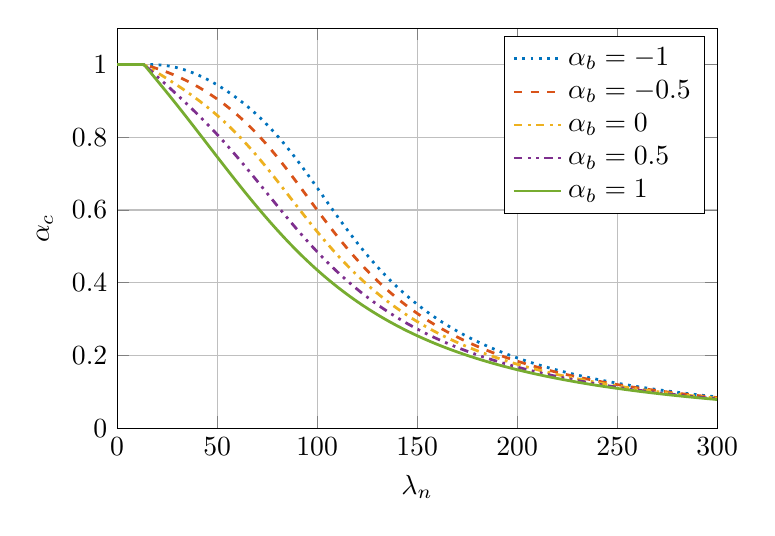
\begin{tikzpicture}

\begin{axis}[%
width=3in,
height=2in,
scale only axis,
unbounded coords=jump,
xmin=0,
xmax=300,
ymin=0,
ymax=1.1,
grid=both,
axis background/.style={fill=white},
legend style={legend cell align=left, align=left},
every axis plot/.append style={line width=1pt},
xlabel={$\lambda_n$},
ylabel={$\alpha_c$}
]
\addplot [color=mycolor1,dotted]
  table[row sep=crcr]{%
0	1\\
1	1\\
2	1\\
3	1\\
4	1\\
5	1\\
6	1\\
7	1\\
8	1\\
9	1\\
10	1\\
11	1\\
12	1\\
13	1\\
14	1\\
15	0.999999999999999\\
16	1\\
17	1\\
18	1\\
19	0.999824384701371\\
20	0.999555120009534\\
21	0.999196477765659\\
22	0.998743459803776\\
23	0.998191808169714\\
24	0.997537992249513\\
25	0.996779185537681\\
26	0.995913233184911\\
27	0.994938611616997\\
28	0.993854381618564\\
29	0.992660136325684\\
30	0.991355945571908\\
31	0.989942297987043\\
32	0.988420042162727\\
33	0.986790328081354\\
34	0.985054549863179\\
35	0.983214290729226\\
36	0.981271270913012\\
37	0.979227299089589\\
38	0.977084227732418\\
39	0.974843912661934\\
40	0.972508176918371\\
41	0.97007877897763\\
42	0.967557385233927\\
43	0.964945546596907\\
44	0.962244678992967\\
45	0.959456047519637\\
46	0.956580753976014\\
47	0.953619727479743\\
48	0.95057371787953\\
49	0.94744329167986\\
50	0.944228830209306\\
51	0.94093052978395\\
52	0.937548403641314\\
53	0.934082285446479\\
54	0.930531834199619\\
55	0.926896540402068\\
56	0.923175733365412\\
57	0.919368589574482\\
58	0.915474142039885\\
59	0.911491290598588\\
60	0.90741881314165\\
61	0.903255377766273\\
62	0.898999555864643\\
63	0.894649836174361\\
64	0.890204639824305\\
65	0.885662336415394\\
66	0.881021261177567\\
67	0.876279733242094\\
68	0.871436075061882\\
69	0.8664886330013\\
70	0.861435799101147\\
71	0.856276034003272\\
72	0.851007890993198\\
73	0.845630041087574\\
74	0.840141299056808\\
75	0.834540650231982\\
76	0.828827277899883\\
77	0.823000591041529\\
78	0.817060252119239\\
79	0.811006204566613\\
80	0.804838699586873\\
81	0.798558321819891\\
82	0.792166013399713\\
83	0.785663095894972\\
84	0.779051289607148\\
85	0.772332729698715\\
86	0.765509978637178\\
87	0.758586034473548\\
88	0.751564334526061\\
89	0.744448754111874\\
90	0.737243600060331\\
91	0.729953598848867\\
92	0.722583879323696\\
93	0.715139950097653\\
94	0.707627671851988\\
95	0.700053224901737\\
96	0.692423072509736\\
97	0.684743920546596\\
98	0.677022674187964\\
99	0.66926639241183\\
100	0.661482241104616\\
101	0.653677445603552\\
102	0.64585924349444\\
103	0.638034838449515\\
104	0.630211355832435\\
105	0.622395800720122\\
106	0.614595018898583\\
107	0.606815661286902\\
108	0.599064152135055\\
109	0.591346661231929\\
110	0.583669080253948\\
111	0.576037003285698\\
112	0.568455711454667\\
113	0.560930161544567\\
114	0.553464978386999\\
115	0.54606445077974\\
116	0.538732530641661\\
117	0.531472835088363\\
118	0.524288651098088\\
119	0.517182942432917\\
120	0.510158358484243\\
121	0.503217244722432\\
122	0.496361654447016\\
123	0.489593361554239\\
124	0.482913874062015\\
125	0.476324448157255\\
126	0.469826102556127\\
127	0.463419632993328\\
128	0.457105626681244\\
129	0.450884476603521\\
130	0.444756395529689\\
131	0.438721429657846\\
132	0.432779471810972\\
133	0.426930274129009\\
134	0.421173460213597\\
135	0.415508536695207\\
136	0.40993490420356\\
137	0.404451867731741\\
138	0.399058646392404\\
139	0.393754382571169\\
140	0.388538150487723\\
141	0.383408964179532\\
142	0.378365784926496\\
143	0.373407528137471\\
144	0.3685330697215\\
145	0.363741251967885\\
146	0.359030888960013\\
147	0.354400771548225\\
148	0.349849671907038\\
149	0.345376347701746\\
150	0.340979545888945\\
151	0.336658006174861\\
152	0.332410464154536\\
153	0.328235654154021\\
154	0.324132311796783\\
155	0.32009917631444\\
156	0.31613499262097\\
157	0.312238513168421\\
158	0.308408499601137\\
159	0.304643724224473\\
160	0.300942971302949\\
161	0.297305038201856\\
162	0.293728736385342\\
163	0.290212892283151\\
164	0.286756348037292\\
165	0.283357962139146\\
166	0.280016609966707\\
167	0.27673118423096\\
168	0.273500595339709\\
169	0.270323771686517\\
170	0.267199659871839\\
171	0.26412722486287\\
172	0.261105450098094\\
173	0.258133337542039\\
174	0.255209907695325\\
175	0.252334199564616\\
176	0.249505270596754\\
177	0.246722196580962\\
178	0.243984071522686\\
179	0.241290007492327\\
180	0.238639134451855\\
181	0.236030600061997\\
182	0.2334635694725\\
183	0.230937225097702\\
184	0.228450766379466\\
185	0.226003409539354\\
186	0.223594387321704\\
187	0.221222948729171\\
188	0.218888358752098\\
189	0.216589898092985\\
190	0.214326862887181\\
191	0.212098564420818\\
192	0.209904328846924\\
193	0.207743496900503\\
194	0.205615423613367\\
195	0.203519478029342\\
196	0.201455042920459\\
197	0.199421514504651\\
198	0.197418302165418\\
199	0.195444828173867\\
200	0.193500527413505\\
201	0.191584847108076\\
202	0.189697246552743\\
203	0.187837196848834\\
204	0.18600418064237\\
205	0.184197691866539\\
206	0.182417235488272\\
207	0.180662327259033\\
208	0.178932493469927\\
209	0.177227270711207\\
210	0.175546205636229\\
211	0.173888854729908\\
212	0.172254784081704\\
213	0.17064356916314\\
214	0.169054794609869\\
215	0.167488054008276\\
216	0.165942949686594\\
217	0.164419092510519\\
218	0.16291610168327\\
219	0.161433604550085\\
220	0.159971236407071\\
221	0.15852864031439\\
222	0.157105466913697\\
223	0.155701374249798\\
224	0.154316027596441\\
225	0.15294909928619\\
226	0.151600268544313\\
227	0.150269221326604\\
228	0.148955650161086\\
229	0.147659253993499\\
230	0.146379738036527\\
231	0.14511681362267\\
232	0.143870198060691\\
233	0.14263961449557\\
234	0.141424791771887\\
235	0.140225464300562\\
236	0.139041371928864\\
237	0.137872259813648\\
238	0.136717878297705\\
239	0.135577982789196\\
240	0.134452333644059\\
241	0.133340696051354\\
242	0.132242839921447\\
243	0.131158539776988\\
244	0.130087574646602\\
245	0.129029727961227\\
246	0.127984787453044\\
247	0.126952545056925\\
248	0.125932796814342\\
249	0.12492534277967\\
250	0.123929986928833\\
251	0.122946537070223\\
252	0.121974804757843\\
253	0.121014605206617\\
254	0.120065757209799\\
255	0.119128083058449\\
256	0.118201408462902\\
257	0.117285562476195\\
258	0.116380377419385\\
259	0.115485688808728\\
260	0.114601335284655\\
261	0.113727158542504\\
262	0.112863003264968\\
263	0.1120087170562\\
264	0.111164150377548\\
265	0.11032915648487\\
266	0.109503591367381\\
267	0.108687313688006\\
268	0.107880184725191\\
269	0.10708206831613\\
270	0.106292830801384\\
271	0.105512340970843\\
272	0.104740470010999\\
273	0.103977091453506\\
274	0.103222081124971\\
275	0.102475317097974\\
276	0.101736679643251\\
277	0.101006051183044\\
278	0.100283316245557\\
279	0.0995683614205096\\
280	0.0988610753157531\\
281	0.0981613485149178\\
282	0.0974690735360702\\
283	0.0967841447913511\\
284	0.0961064585475702\\
285	0.095435912887731\\
286	0.0947724076734636\\
287	0.0941158445083413\\
288	0.0934661267020572\\
289	0.0928231592354404\\
290	0.0921868487262887\\
291	0.091557103395998\\
292	0.0909338330369663\\
293	0.0903169489807545\\
294	0.0897063640669837\\
295	0.0891019926129488\\
296	0.088503750383933\\
297	0.0879115545642027\\
298	0.0873253237286678\\
299	0.0867449778151878\\
300	0.0861704380975105\\
};
\addlegendentry{$\alpha_b=-1$}

\addplot [color=mycolor2,dashed]
  table[row sep=crcr]{%
0	1\\
1	1\\
2	1\\
3	1\\
4	1\\
5	1\\
6	1\\
7	1\\
8	1\\
9	1\\
10	1\\
11	1\\
12	1\\
13	1\\
14	0.999194221569034\\
15	0.997565219315693\\
16	0.995908980215453\\
17	0.994220956670302\\
18	0.992496876355957\\
19	0.990732758417115\\
20	0.988924923893506\\
21	0.987070000472851\\
22	0.985164921825223\\
23	0.983206921909146\\
24	0.981193524748871\\
25	0.979122530263222\\
26	0.976991996778537\\
27	0.974800220883251\\
28	0.972545715281573\\
29	0.970227185282367\\
30	0.967843504520164\\
31	0.965393690452787\\
32	0.962876880118326\\
33	0.960292306567062\\
34	0.957639276314992\\
35	0.954917148097725\\
36	0.952125313139168\\
37	0.949263177090299\\
38	0.946330143740794\\
39	0.943325600560864\\
40	0.940248906092917\\
41	0.937099379182173\\
42	0.933876290012109\\
43	0.930578852893744\\
44	0.927206220746826\\
45	0.923757481204985\\
46	0.920231654275193\\
47	0.916627691483564\\
48	0.912944476443865\\
49	0.909180826791345\\
50	0.905335497431966\\
51	0.901407185065255\\
52	0.897394533947076\\
53	0.893296142866339\\
54	0.889110573316378\\
55	0.884836358847067\\
56	0.88047201558738\\
57	0.876016053929489\\
58	0.871466991364565\\
59	0.866823366456596\\
60	0.862083753933763\\
61	0.857246780866832\\
62	0.85231114389055\\
63	0.847275627407002\\
64	0.842139122689512\\
65	0.836900647781716\\
66	0.831559368059644\\
67	0.826114617294971\\
68	0.820565919026086\\
69	0.814913008010745\\
70	0.809155851501162\\
71	0.803294670050422\\
72	0.797329957529694\\
73	0.791262500010386\\
74	0.78509339314571\\
75	0.778824057674035\\
76	0.772456252663242\\
77	0.765992086122842\\
78	0.759434022629708\\
79	0.752784887645046\\
80	0.746047868244568\\
81	0.739226510040764\\
82	0.732324710144358\\
83	0.725346706090092\\
84	0.718297060737419\\
85	0.71118064324667\\
86	0.704002606322589\\
87	0.696768360006033\\
88	0.68948354237777\\
89	0.682153987611999\\
90	0.674785691878586\\
91	0.667384777639479\\
92	0.659957456914615\\
93	0.652509994105039\\
94	0.645048668955676\\
95	0.63757974021828\\
96	0.630109410537847\\
97	0.62264379303563\\
98	0.615188880001246\\
99	0.607750514038396\\
100	0.600334361936172\\
101	0.592945891463996\\
102	0.585590351215371\\
103	0.578272753556382\\
104	0.570997860671046\\
105	0.563770173638677\\
106	0.556593924429467\\
107	0.549473070663818\\
108	0.542411292948982\\
109	0.53541199458283\\
110	0.5284783033987\\
111	0.521613075516579\\
112	0.514818900763389\\
113	0.508098109528144\\
114	0.501452780825104\\
115	0.494884751348975\\
116	0.488395625319787\\
117	0.481986784930476\\
118	0.475659401226861\\
119	0.469414445266827\\
120	0.46325269942279\\
121	0.457174768708404\\
122	0.451181092026736\\
123	0.445271953252452\\
124	0.439447492074882\\
125	0.43370771454198\\
126	0.428052503257081\\
127	0.422481627191125\\
128	0.416994751082457\\
129	0.411591444404707\\
130	0.406271189890478\\
131	0.401033391604788\\
132	0.395877382567502\\
133	0.390802431928434\\
134	0.385807751702401\\
135	0.380892503074532\\
136	0.376055802288463\\
137	0.371296726131857\\
138	0.366614317035097\\
139	0.362007587799913\\
140	0.357475525975358\\
141	0.353017097898881\\
142	0.348631252420344\\
143	0.344316924326722\\
144	0.340073037484988\\
145	0.335898507720269\\
146	0.331792245445905\\
147	0.327753158061435\\
148	0.323780152133957\\
149	0.319872135377611\\
150	0.316028018445248\\
151	0.312246716545686\\
152	0.308527150899181\\
153	0.304868250043105\\
154	0.301268950999089\\
155	0.297728200312245\\
156	0.294244954972388\\
157	0.290818183226602\\
158	0.287446865291836\\
159	0.284129993975663\\
160	0.280866575212782\\
161	0.27765562852432\\
162	0.274496187406469\\
163	0.271387299654569\\
164	0.268328027628274\\
165	0.265317448463018\\
166	0.262354654232652\\
167	0.259438752067701\\
168	0.256568864233391\\
169	0.253744128171262\\
170	0.250963696507889\\
171	0.248226737033953\\
172	0.245532432656645\\
173	0.242879981328162\\
174	0.240268595952816\\
175	0.237697504275065\\
176	0.235165948750618\\
177	0.232673186402543\\
178	0.230218488664182\\
179	0.227801141210502\\
180	0.225420443779386\\
181	0.223075709984221\\
182	0.220766267119046\\
183	0.218491455957387\\
184	0.216250630545819\\
185	0.214043157993202\\
186	0.211868418256443\\
187	0.209725803923566\\
188	0.207614719994794\\
189	0.205534583662274\\
190	0.203484824089036\\
191	0.201464882187684\\
192	0.199474210399313\\
193	0.197512272473038\\
194	0.19557854324655\\
195	0.19367250842799\\
196	0.191793664379484\\
197	0.189941517902568\\
198	0.188115586025759\\
199	0.186315395794465\\
200	0.184540484063427\\
201	0.182790397291831\\
202	0.181064691341247\\
203	0.17936293127649\\
204	0.177684691169517\\
205	0.176029553906432\\
206	0.174397110997665\\
207	0.172786962391386\\
208	0.171198716290194\\
209	0.169631988971095\\
210	0.168086404608824\\
211	0.166561595102478\\
212	0.165057199905508\\
213	0.163572865859028\\
214	0.16210824702846\\
215	0.160663004543481\\
216	0.159236806441258\\
217	0.157829327512942\\
218	0.156440249153398\\
219	0.155069259214124\\
220	0.153716051859341\\
221	0.152380327425193\\
222	0.151061792282039\\
223	0.149760158699766\\
224	0.148475144716108\\
225	0.147206474007893\\
226	0.145953875765195\\
227	0.144717084568326\\
228	0.143495840267625\\
229	0.142289887865989\\
230	0.141098977404101\\
231	0.139922863848293\\
232	0.138761306981008\\
233	0.137614071293793\\
234	0.136480925882778\\
235	0.135361644346598\\
236	0.134256004686693\\
237	0.13316378920994\\
238	0.132084784433575\\
239	0.13101878099234\\
240	0.129965573547823\\
241	0.128924960699924\\
242	0.127896744900414\\
243	0.126880732368535\\
244	0.125876733008586\\
245	0.124884560329463\\
246	0.123904031366101\\
247	0.122934966602764\\
248	0.121977189898165\\
249	0.12103052841234\\
250	0.120094812535262\\
251	0.11916987581714\\
252	0.118255554900363\\
253	0.117351689453052\\
254	0.116458122104184\\
255	0.115574698380243\\
256	0.114701266643368\\
257	0.113837678030952\\
258	0.112983786396672\\
259	0.112139448252897\\
260	0.111304522714454\\
261	0.110478871443711\\
262	0.109662358596951\\
263	0.108854850771993\\
264	0.108056216957048\\
265	0.107266328480765\\
266	0.106485058963434\\
267	0.10571228426934\\
268	0.104947882460211\\
269	0.104191733749754\\
270	0.103443720459241\\
271	0.102703726974126\\
272	0.10197163970166\\
273	0.101247347029486\\
274	0.100530739285185\\
275	0.0998217086967541\\
276	0.0991201493539868\\
277	0.0984259571707414\\
278	0.0977390298480688\\
279	0.0970592668381817\\
280	0.0963865693092443\\
281	0.0957208401109605\\
282	0.0950619837409435\\
283	0.0944099063118445\\
284	0.0937645155192248\\
285	0.0931257206101506\\
286	0.0924934323524944\\
287	0.0918675630049243\\
288	0.0912480262875657\\
289	0.0906347373533175\\
290	0.0900276127598082\\
291	0.089426570441975\\
292	0.0888315296852514\\
293	0.0882424110993486\\
294	0.0876591365926153\\
295	0.0870816293469634\\
296	0.0865098137933441\\
297	0.0859436155877625\\
298	0.0853829615878171\\
299	0.0848277798297508\\
300	0.0842779995060027\\
};
\addlegendentry{$\alpha_b=-0.5$}

\addplot [color=mycolor3,dash dot]
  table[row sep=crcr]{%
0	1\\
1	1\\
2	1\\
3	1\\
4	1\\
5	1\\
6	1\\
7	1\\
8	1\\
9	1\\
10	1\\
11	1\\
12	1\\
13	1\\
14	0.998332434450888\\
15	0.994996168935598\\
16	0.991656503959234\\
17	0.98831119910115\\
18	0.984958037515687\\
19	0.981594822090769\\
20	0.978219371887404\\
21	0.974829518849201\\
22	0.971423104773862\\
23	0.967997978541497\\
24	0.964551993597314\\
25	0.961083005688876\\
26	0.957588870860729\\
27	0.954067443711749\\
28	0.950516575923061\\
29	0.946934115066923\\
30	0.943317903709393\\
31	0.939665778822103\\
32	0.935975571520841\\
33	0.932245107151051\\
34	0.928472205742642\\
35	0.924654682858737\\
36	0.920790350865028\\
37	0.916877020648354\\
38	0.912912503814719\\
39	0.90889461539838\\
40	0.90482117711459\\
41	0.900690021189082\\
42	0.896498994797333\\
43	0.892245965145909\\
44	0.887928825226624\\
45	0.883545500271773\\
46	0.879093954935148\\
47	0.874572201218756\\
48	0.869978307159016\\
49	0.865310406278666\\
50	0.860566707801273\\
51	0.855745507614459\\
52	0.850845199955184\\
53	0.845864289776015\\
54	0.84080140573517\\
55	0.835655313735266\\
56	0.830424930916535\\
57	0.825109339989885\\
58	0.819707803774042\\
59	0.814219779779685\\
60	0.808644934662421\\
61	0.802983158346469\\
62	0.797234577602846\\
63	0.791399568850455\\
64	0.785478769936733\\
65	0.779473090647398\\
66	0.773383721693113\\
67	0.767212141925424\\
68	0.76096012354575\\
69	0.754629735089899\\
70	0.748223341996751\\
71	0.741743604603284\\
72	0.735193473448399\\
73	0.728576181814454\\
74	0.721895235486627\\
75	0.715154399764879\\
76	0.708357683819652\\
77	0.701509322538542\\
78	0.69461375606513\\
79	0.687675607280952\\
80	0.680699657525402\\
81	0.673690820884592\\
82	0.666654117407642\\
83	0.659594645626481\\
84	0.652517554762737\\
85	0.645428017002574\\
86	0.63833120020781\\
87	0.631232241410195\\
88	0.624136221406461\\
89	0.617048140736117\\
90	0.609972897283398\\
91	0.602915265701176\\
92	0.595879878809266\\
93	0.588871211074378\\
94	0.58189356423491\\
95	0.574951055092453\\
96	0.568047605453849\\
97	0.561186934173956\\
98	0.554372551220162\\
99	0.547607753655441\\
100	0.540895623417558\\
101	0.5342390267575\\
102	0.527640615190294\\
103	0.521102827805587\\
104	0.514627894783259\\
105	0.508217841960447\\
106	0.501874496300181\\
107	0.495599492117787\\
108	0.489394277928959\\
109	0.483260123792344\\
110	0.477198129029306\\
111	0.471209230213905\\
112	0.465294209336636\\
113	0.45945370205601\\
114	0.453688205962284\\
115	0.447998088787514\\
116	0.442383596505419\\
117	0.436844861273236\\
118	0.431381909175821\\
119	0.425994667739563\\
120	0.42068297319035\\
121	0.415446577435771\\
122	0.410285154757017\\
123	0.40519830820059\\
124	0.400185575663979\\
125	0.395246435672921\\
126	0.390380312850866\\
127	0.385586583083737\\
128	0.380864578385168\\
129	0.376213591469106\\
130	0.371632880038013\\
131	0.367121670795999\\
132	0.362679163196991\\
133	0.358304532938663\\
134	0.353996935213224\\
135	0.349755507726396\\
136	0.345579373496011\\
137	0.341467643441597\\
138	0.337419418776248\\
139	0.333433793211824\\
140	0.329509854988282\\
141	0.325646688737623\\
142	0.321843377192586\\
143	0.318099002749815\\
144	0.314412648896868\\
145	0.310783401511963\\
146	0.307210350045001\\
147	0.303692588587912\\
148	0.300229216842021\\
149	0.296819340989658\\
150	0.293462074476868\\
151	0.290156538713668\\
152	0.286901863697921\\
153	0.283697188568525\\
154	0.280541662093271\\
155	0.277434443096377\\
156	0.274374700830384\\
157	0.271361615296805\\
158	0.268394377519616\\
159	0.265472189775399\\
160	0.262594265783706\\
161	0.259759830860943\\
162	0.256968122040867\\
163	0.25421838816455\\
164	0.251509889942471\\
165	0.248841899991208\\
166	0.246213702847015\\
167	0.2436245949584\\
168	0.241073884659679\\
169	0.238560892127317\\
170	0.236084949320725\\
171	0.233645399909091\\
172	0.231241599185655\\
173	0.228872913970761\\
174	0.226538722504906\\
175	0.22423841433291\\
176	0.221971390180236\\
177	0.219737061822421\\
178	0.217534851948486\\
179	0.215364194019132\\
180	0.213224532120458\\
181	0.211115320813881\\
182	0.209036024982871\\
183	0.206986119677071\\
184	0.204965089954325\\
185	0.202972430721071\\
186	0.201007646571556\\
187	0.199070251626235\\
188	0.197159769369734\\
189	0.19527573248869\\
190	0.19341768270976\\
191	0.191585170638075\\
192	0.189777755596366\\
193	0.187995005464978\\
194	0.186236496522977\\
195	0.184501813290507\\
196	0.182790548372571\\
197	0.181102302304346\\
198	0.179436683398178\\
199	0.177793307592355\\
200	0.176171798301748\\
201	0.174571786270401\\
202	0.172992909426147\\
203	0.171434812737306\\
204	0.169897148071508\\
205	0.168379574056698\\
206	0.16688175594434\\
207	0.165403365474861\\
208	0.163944080745341\\
209	0.162503586079482\\
210	0.161081571899837\\
211	0.159677734602337\\
212	0.158291776433083\\
213	0.156923405367421\\
214	0.155572334991279\\
215	0.154238284384761\\
216	0.152920978007982\\
217	0.15162014558912\\
218	0.150335522014683\\
219	0.149066847221943\\
220	0.147813866093542\\
221	0.146576328354224\\
222	0.145353988469675\\
223	0.144146605547444\\
224	0.142953943239912\\
225	0.141775769649284\\
226	0.140611857234568\\
227	0.139461982720517\\
228	0.138325927008495\\
229	0.137203475089238\\
230	0.136094415957483\\
231	0.134998542528418\\
232	0.133915651555939\\
233	0.132845543552665\\
234	0.131788022711687\\
235	0.130742896830015\\
236	0.129709977233694\\
237	0.128689078704548\\
238	0.12768001940853\\
239	0.126682620825638\\
240	0.125696707681374\\
241	0.124722107879699\\
242	0.123758652437474\\
243	0.122806175420332\\
244	0.121864513879978\\
245	0.120933507792861\\
246	0.120013000000203\\
247	0.119102836149354\\
248	0.118202864636444\\
249	0.1173129365503\\
250	0.116432905617602\\
251	0.115562628149255\\
252	0.114701962987943\\
253	0.11385077145685\\
254	0.1130089173095\\
255	0.112176266680721\\
256	0.111352688038682\\
257	0.110538052137992\\
258	0.109732231973833\\
259	0.108935102737104\\
260	0.108146541770557\\
261	0.107366428525891\\
262	0.106594644521797\\
263	0.105831073302921\\
264	0.105075600399732\\
265	0.104328113289263\\
266	0.103588501356719\\
267	0.102856655857921\\
268	0.102132469882576\\
269	0.10141583831834\\
270	0.100706657815674\\
271	0.100004826753459\\
272	0.0993102452053602\\
273	0.0986228149069229\\
274	0.0979424392233799\\
275	0.0972690231181575\\
276	0.0966024731220605\\
277	0.0959426973031238\\
278	0.0952896052371128\\
279	0.0946431079786585\\
280	0.0940031180330126\\
281	0.0933695493284088\\
282	0.092742317189014\\
283	0.0921213383084596\\
284	0.0915065307239357\\
285	0.0908978137908377\\
286	0.0902951081579512\\
287	0.0896983357431641\\
288	0.0891074197096919\\
289	0.0885222844428063\\
290	0.0879428555270545\\
291	0.0873690597239576\\
292	0.0868008249501786\\
293	0.0862380802561472\\
294	0.0856807558051328\\
295	0.0851287828527541\\
296	0.0845820937269161\\
297	0.0840406218081649\\
298	0.0835043015104489\\
299	0.0829730682622813\\
300	0.082446858488289\\
};
\addlegendentry{$\alpha_b=0$}

\addplot [color=mycolor4,dash dot dot]
  table[row sep=crcr]{%
0	1\\
1	1\\
2	1\\
3	1\\
4	1\\
5	1\\
6	1\\
7	1\\
8	1\\
9	1\\
10	1\\
11	1\\
12	1\\
13	1\\
14	0.997470571631435\\
15	0.992425102547918\\
16	0.98739488247899\\
17	0.982376900317749\\
18	0.977368261000045\\
19	0.972366174705787\\
20	0.967367946412372\\
21	0.962370965805545\\
22	0.957372697592879\\
23	0.95237067229656\\
24	0.947362477624887\\
25	0.942345750535968\\
26	0.937318170112716\\
27	0.932277451366357\\
28	0.92722134007734\\
29	0.922147608768855\\
30	0.917054053890658\\
31	0.911938494270644\\
32	0.906798770870081\\
33	0.901632747856382\\
34	0.896438314985929\\
35	0.891213391269222\\
36	0.88595592987206\\
37	0.880663924189857\\
38	0.875335415017547\\
39	0.869968498724893\\
40	0.864561336336103\\
41	0.859112163403366\\
42	0.853619300555892\\
43	0.848081164599012\\
44	0.842496280031734\\
45	0.836863290845549\\
46	0.831180972462179\\
47	0.825448243663371\\
48	0.819664178361756\\
49	0.813828017058337\\
50	0.807939177829622\\
51	0.801997266686055\\
52	0.79600208714341\\
53	0.789953648850754\\
54	0.783852175122677\\
55	0.777698109230051\\
56	0.771492119313035\\
57	0.765235101792421\\
58	0.758928183170982\\
59	0.752572720135118\\
60	0.746170297888736\\
61	0.739722726675599\\
62	0.733232036472973\\
63	0.726700469867668\\
64	0.720130473154877\\
65	0.713524685729799\\
66	0.706885927871011\\
67	0.700217187042123\\
68	0.693521602863612\\
69	0.68680245092896\\
70	0.680063125657868\\
71	0.673307122393589\\
72	0.666538018961137\\
73	0.65975945690791\\
74	0.65297512264815\\
75	0.646188728727819\\
76	0.639403995417076\\
77	0.632624632824215\\
78	0.625854323708082\\
79	0.619096707146408\\
80	0.612355363195741\\
81	0.60563379865568\\
82	0.59893543402629\\
83	0.592263591723972\\
84	0.585621485597911\\
85	0.579012211767346\\
86	0.572438740779528\\
87	0.565903911069828\\
88	0.559410423689179\\
89	0.552960838250062\\
90	0.546557570030634\\
91	0.540202888167325\\
92	0.533898914859185\\
93	0.527647625502384\\
94	0.521450849670287\\
95	0.515310272853304\\
96	0.509227438873059\\
97	0.503203752887002\\
98	0.497240484902325\\
99	0.491338773721621\\
100	0.485499631246948\\
101	0.479723947073783\\
102	0.47401249331134\\
103	0.468365929571095\\
104	0.462784808070609\\
105	0.457269578805107\\
106	0.451820594744399\\
107	0.446438117017748\\
108	0.441122320054009\\
109	0.435873296648872\\
110	0.430691062935152\\
111	0.425575563235992\\
112	0.420526674784296\\
113	0.415544212294974\\
114	0.410627932379436\\
115	0.405777537794369\\
116	0.400992681519121\\
117	0.396272970658038\\
118	0.391617970165858\\
119	0.387027206395812\\
120	0.382500170471361\\
121	0.378036321483649\\
122	0.373635089517652\\
123	0.369295878510797\\
124	0.365018068948441\\
125	0.360801020401114\\
126	0.356644073908791\\
127	0.352546554217794\\
128	0.348507771876066\\
129	0.344527025192744\\
130	0.34060360206799\\
131	0.336736781699053\\
132	0.332925836168507\\
133	0.329170031920529\\
134	0.325468631130974\\
135	0.321820892976876\\
136	0.318226074810848\\
137	0.314683433245677\\
138	0.31119222515425\\
139	0.307751708589727\\
140	0.304361143630713\\
141	0.301019793155948\\
142	0.297726923552863\\
143	0.294481805364127\\
144	0.291283713876132\\
145	0.288131929653143\\
146	0.285025739020668\\
147	0.281964434501418\\
148	0.278947315207021\\
149	0.275973687188517\\
150	0.273042863748453\\
151	0.270154165717268\\
152	0.267306921696486\\
153	0.264500468271077\\
154	0.261734150193234\\
155	0.25900732053965\\
156	0.256319340844261\\
157	0.253669581208304\\
158	0.251057420389422\\
159	0.248482245871418\\
160	0.245943453916194\\
161	0.243440449599282\\
162	0.240972646830289\\
163	0.238539468359502\\
164	0.236140345771803\\
165	0.233774719468967\\
166	0.231442038641367\\
167	0.229141761229997\\
168	0.226873353879709\\
169	0.224636291884459\\
170	0.222430059125331\\
171	0.22025414800203\\
172	0.218108059358512\\
173	0.215991302403333\\
174	0.213903394625315\\
175	0.211843861705009\\
176	0.209812237422479\\
177	0.20780806356183\\
178	0.205830889812892\\
179	0.203880273670471\\
180	0.201955780331488\\
181	0.200056982590358\\
182	0.198183460732893\\
183	0.196334802429023\\
184	0.19451060262458\\
185	0.192710463432382\\
186	0.190933994022843\\
187	0.189180810514288\\
188	0.18745053586318\\
189	0.185742799754403\\
190	0.184057238491762\\
191	0.18239349488885\\
192	0.180751218160379\\
193	0.179130063814125\\
194	0.177529693543563\\
195	0.175949775121299\\
196	0.174389982293381\\
197	0.172849994674566\\
198	0.171329497644606\\
199	0.169828182245626\\
200	0.168345745080627\\
201	0.166881888213187\\
202	0.165436319068376\\
203	0.164008750334947\\
204	0.162598899868809\\
205	0.161206490597829\\
206	0.159831250427972\\
207	0.158472912150804\\
208	0.157131213352376\\
209	0.155805896323486\\
210	0.154496707971348\\
211	0.153203399732656\\
212	0.151925727488053\\
213	0.150663451478014\\
214	0.149416336220121\\
215	0.148184150427753\\
216	0.146966666930157\\
217	0.145763662593924\\
218	0.144574918245835\\
219	0.143400218597079\\
220	0.142239352168842\\
221	0.14109211121923\\
222	0.139958291671543\\
223	0.138837693043857\\
224	0.137730118379928\\
225	0.136635374181379\\
226	0.135553270341169\\
227	0.134483620078321\\
228	0.133426239873892\\
229	0.132380949408178\\
230	0.131347571499121\\
231	0.130325932041908\\
232	0.129315859949754\\
233	0.128317187095823\\
234	0.127329748256309\\
235	0.126353381054614\\
236	0.125387925906648\\
237	0.124433225967191\\
238	0.123489127077339\\
239	0.122555477712979\\
240	0.121632128934303\\
241	0.120718934336323\\
242	0.119815750000385\\
243	0.11892243444665\\
244	0.118038848587529\\
245	0.117164855682061\\
246	0.116300321291208\\
247	0.11544511323405\\
248	0.114599101544868\\
249	0.113762158431092\\
250	0.112934158232107\\
251	0.112114977378884\\
252	0.111304494354434\\
253	0.110502589655067\\
254	0.109709145752432\\
255	0.108924047056331\\
256	0.108147179878282\\
257	0.10737843239583\\
258	0.106617694617579\\
259	0.10586485834893\\
260	0.105119817158521\\
261	0.104382466345345\\
262	0.103652702906533\\
263	0.102930425505797\\
264	0.102215534442507\\
265	0.101507931621396\\
266	0.100807520522879\\
267	0.100114206173978\\
268	0.0994278951198246\\
269	0.098748495395748\\
270	0.0980759164999236\\
271	0.0974100693665737\\
272	0.0967508663397091\\
273	0.0960982211473998\\
274	0.0954520488765637\\
275	0.0948122659482631\\
276	0.0941787900934965\\
277	0.0935515403294774\\
278	0.0929304369363879\\
279	0.0923154014345987\\
280	0.0917063565623442\\
281	0.0911032262538441\\
282	0.0905059356178613\\
283	0.0899144109166876\\
284	0.0893285795455475\\
285	0.0887483700124113\\
286	0.088173711918209\\
287	0.0876045359374373\\
288	0.0870407737991488\\
289	0.0864823582683191\\
290	0.0859292231275804\\
291	0.0853813031593149\\
292	0.0848385341281022\\
293	0.0843008527635102\\
294	0.0837681967432238\\
295	0.0832405046765053\\
296	0.0827177160879768\\
297	0.0821997714017203\\
298	0.0816866119256877\\
299	0.0811781798364134\\
300	0.0806744181640256\\
};
\addlegendentry{$\alpha_b=0.5$}

\addplot [color=mycolor5]
  table[row sep=crcr]{%
0	1\\
1	1\\
2	1\\
3	1\\
4	1\\
5	1\\
6	1\\
7	1\\
8	1\\
9	1\\
10	1\\
11	1\\
12	1\\
13	1\\
14	0.99660859379397\\
15	0.989850996135561\\
16	0.983119542274831\\
17	0.976405954452022\\
18	0.969702732861994\\
19	0.963003139693162\\
20	0.956301182161364\\
21	0.949591593670344\\
22	0.94286981246087\\
23	0.936131957327269\\
24	0.929374800182193\\
25	0.922595735435773\\
26	0.915792746321894\\
27	0.908964368449735\\
28	0.902109650980842\\
29	0.89522811592916\\
30	0.888319716152307\\
31	0.881384792646684\\
32	0.874424031776987\\
33	0.86743842306372\\
34	0.860429218122406\\
35	0.853397891298326\\
36	0.846346102474143\\
37	0.839275662448752\\
38	0.832188501198262\\
39	0.825086639238297\\
40	0.817972162214982\\
41	0.810847198763459\\
42	0.803713901590976\\
43	0.796574431668752\\
44	0.789430945354954\\
45	0.782285584221291\\
46	0.775140467318417\\
47	0.767997685590437\\
48	0.760859298135647\\
49	0.753727330008297\\
50	0.746603771263057\\
51	0.739490576958835\\
52	0.732389667859631\\
53	0.725302931595937\\
54	0.718232224079048\\
55	0.711179370991235\\
56	0.704146169205755\\
57	0.69713438802106\\
58	0.690145770122535\\
59	0.683182032211789\\
60	0.676244865267725\\
61	0.66933593442479\\
62	0.662456878471849\\
63	0.655609308990146\\
64	0.648794809160652\\
65	0.642014932280112\\
66	0.635271200031432\\
67	0.628565100557935\\
68	0.62189808639283\\
69	0.615271572295202\\
70	0.608686933042335\\
71	0.602145501225433\\
72	0.59564856509216\\
73	0.589197366475093\\
74	0.582793098840392\\
75	0.576436905485986\\
76	0.570129877913491\\
77	0.563873054393039\\
78	0.557667418735391\\
79	0.551513899281143\\
80	0.545413368112637\\
81	0.53936664049038\\
82	0.533374474512355\\
83	0.5274375709917\\
84	0.52155657354563\\
85	0.515732068886429\\
86	0.509964587303589\\
87	0.504254603324857\\
88	0.498602536542962\\
89	0.493008752594098\\
90	0.48747356427389\\
91	0.481997232776365\\
92	0.476579969041571\\
93	0.471221935197684\\
94	0.465923246083875\\
95	0.460683970840713\\
96	0.455504134555501\\
97	0.450383719950616\\
98	0.445322669103701\\
99	0.440320885189293\\
100	0.435378234232296\\
101	0.4304945468645\\
102	0.425669620076135\\
103	0.420903218955248\\
104	0.416195078408418\\
105	0.411544904857082\\
106	0.406952377904417\\
107	0.402417151968395\\
108	0.397938857877233\\
109	0.393517104424033\\
110	0.389151479877978\\
111	0.384841553449873\\
112	0.38058687671037\\
113	0.37638698495952\\
114	0.372241398546777\\
115	0.368149624140826\\
116	0.364111155948984\\
117	0.360125476886141\\
118	0.356192059693473\\
119	0.352310368007369\\
120	0.348479857379197\\
121	0.344699976246678\\
122	0.340970166857801\\
123	0.337289866148301\\
124	0.333658506573843\\
125	0.330075516898102\\
126	0.32654032293804\\
127	0.323052348267668\\
128	0.31961101488169\\
129	0.316215743820378\\
130	0.312865955757111\\
131	0.309561071549951\\
132	0.306300512758701\\
133	0.303083702128803\\
134	0.299910064043495\\
135	0.296779024945573\\
136	0.293690013730097\\
137	0.290642462109384\\
138	0.287635804951535\\
139	0.284669480593786\\
140	0.281742931131878\\
141	0.278855602686646\\
142	0.276006945648959\\
143	0.273196414904136\\
144	0.270423470036894\\
145	0.26768757551787\\
146	0.264988200872708\\
147	0.262324820834663\\
148	0.259696915481639\\
149	0.257103970358544\\
150	0.254545476585804\\
151	0.252020930954833\\
152	0.249529836011236\\
153	0.247071700126488\\
154	0.244646037558767\\
155	0.242252368503635\\
156	0.239890219135189\\
157	0.237559121638298\\
158	0.235258614232482\\
159	0.232988241188013\\
160	0.23074755283473\\
161	0.22853610556407\\
162	0.226353461824794\\
163	0.224199190112834\\
164	0.222072864955692\\
165	0.219974066891788\\
166	0.217902382445126\\
167	0.215857404095646\\
168	0.213838730245579\\
169	0.211845965182146\\
170	0.209878719036875\\
171	0.207936607741843\\
172	0.206019252983085\\
173	0.204126282151436\\
174	0.202257328291046\\
175	0.200412030045764\\
176	0.198590031603634\\
177	0.196790982639672\\
178	0.19501453825712\\
179	0.193260358927349\\
180	0.191528110428567\\
181	0.189817463783497\\
182	0.188128095196143\\
183	0.186459685987809\\
184	0.184811922532463\\
185	0.183184496191582\\
186	0.181577103248589\\
187	0.179989444842959\\
188	0.178421226904118\\
189	0.176872160085198\\
190	0.175341959696751\\
191	0.173830345640472\\
192	0.17233704234303\\
193	0.170861778690042\\
194	0.169404287960279\\
195	0.167964307760131\\
196	0.166541579958412\\
197	0.165135850621519\\
198	0.163746869949021\\
199	0.162374392209688\\
200	0.16101817567802\\
201	0.159677982571294\\
202	0.158353578987161\\
203	0.157044734841831\\
204	0.155751223808853\\
205	0.154472823258524\\
206	0.153209314197951\\
207	0.151960481211764\\
208	0.150726112403517\\
209	0.149505999337777\\
210	0.14829993698292\\
211	0.147107723654643\\
212	0.14592916096019\\
213	0.144764053743318\\
214	0.143612210029998\\
215	0.142473440974849\\
216	0.141347560808324\\
217	0.140234386784642\\
218	0.139133739130457\\
219	0.138045440994291\\
220	0.136969318396702\\
221	0.135905200181205\\
222	0.134852917965931\\
223	0.133812306096034\\
224	0.132783201596834\\
225	0.131765444127687\\
226	0.130758875936599\\
227	0.129763341815548\\
228	0.128778689056541\\
229	0.12780476740837\\
230	0.126841429034086\\
231	0.12588852846917\\
232	0.124945922580395\\
233	0.124013470525378\\
234	0.123091033712815\\
235	0.122178475763376\\
236	0.121275662471277\\
237	0.120382461766503\\
238	0.119498743677676\\
239	0.118624380295568\\
240	0.117759245737242\\
241	0.11690321611082\\
242	0.116056169480862\\
243	0.115217985834352\\
244	0.114388547047281\\
245	0.113567736851825\\
246	0.112755440804095\\
247	0.11195154625246\\
248	0.111155942306443\\
249	0.110368519806154\\
250	0.109589171292287\\
251	0.108817790976643\\
252	0.108054274713182\\
253	0.107298519969605\\
254	0.106550425799432\\
255	0.105809892814601\\
256	0.105076823158547\\
257	0.104351120479778\\
258	0.103632689905926\\
259	0.102921438018265\\
260	0.102217272826701\\
261	0.101520103745207\\
262	0.100829841567707\\
263	0.100146398444406\\
264	0.0994696878585412\\
265	0.0987996246035651\\
266	0.0981361247607381\\
267	0.0974791056771354\\
268	0.096828485944053\\
269	0.0961841853758072\\
270	0.0955461249889242\\
271	0.0949142269817065\\
272	0.0942884147141758\\
273	0.0936686126883797\\
274	0.0930547465290607\\
275	0.0924467429646762\\
276	0.0918445298087677\\
277	0.0912480359416675\\
278	0.0906571912925425\\
279	0.0900719268217634\\
280	0.0894921745035974\\
281	0.0889178673092156\\
282	0.0883489391900109\\
283	0.0877853250612203\\
284	0.0872269607858449\\
285	0.0866737831588631\\
286	0.0861257298917314\\
287	0.0855827395971667\\
288	0.0850447517742056\\
289	0.0845117067935352\\
290	0.0839835458830894\\
291	0.0834602111139075\\
292	0.0829416453862483\\
293	0.0824277924159566\\
294	0.0819185967210751\\
295	0.0814140036086995\\
296	0.0809139591620706\\
297	0.0804184102278988\\
298	0.0799273044039182\\
299	0.0794405900266637\\
300	0.078958216159469\\
};
\addlegendentry{$\alpha_b=1$}

\end{axis}
\end{tikzpicture}%
\caption{$\alpha_c$ as a function of $\lambda_n$}\label{fig:alpha_c}
\end{figure}

Performing such a computation is somehow tedious, in practice, engineers can refer to the pre-compiled table \NZSSTEEL{Table 6.3.3(2)}, as well as \tabref{tab:alpha_c}, to find the proper value to be used.

The most conservative curve is that with $\alpha_b=1$. The European codes, like \NZSSTEEL{}, have five curves for $\alpha_b$. The Canadian code has 3 curves for different residual stress conditions, while the US code has just one curve for all residual stress conditions.
\begin{exmp}
What is the maximum stress that can be applied to a hot-rolled compact Grade 300 column (no holes) with $t_f<\SI{11}{\mm}$ and $\lambda=100$?
\end{exmp}
\begin{solution}
Since it is compact section, shear lag is often not a problem. It can be safely assumed that $k_f=1$. Since there are no holes, $A_n=A_g$. From \tabref{tab:alpha_b}, $\alpha_b=0$ for hot-rolled section. For $t_f<\SI{11}{\mm}$, assume $f_y=\SI{320}{\mpa}$ for Grade 300 steel.

The modified slenderness ratio
\begin{gather*}
\lambda_n=\lambda\sqrt{k_f}\sqrt{\dfrac{f_y}{\SI{250}{\mpa}}}=100\times\sqrt{1}\times\sqrt{\dfrac{320}{250}}=113.1.
\end{gather*}

$\alpha_c$ can be computed (or found from \tabref{tab:alpha_c}, or \figref{fig:alpha_c}) as \num{0.459}. Thus, the maximum stress is
\begin{gather*}
f_{max}=\dfrac{N^*}{A_n}\leqslant\dfrac{\phi{}N_c}{A_n}=\phi\alpha_ck_ff_y=0.9\times0.459\times1\times\SI{320}{\mpa}=\SI{132.2}{\mpa}.
\end{gather*}
\end{solution}
\begin{table}[H]
\centering\scriptsize\setlength{\tabcolsep}{4pt}\renewcommand{\arraystretch}{1.03}
\caption{Values of $\alpha_c$ as function of $\alpha_b$ and $\lambda_n$}\label{tab:alpha_c}
\begin{tabular}{c|ccccc|c|ccccc|c|ccccc}
	\toprule
	            &    \multicolumn{5}{c|}{$\alpha_b$}    &             &    \multicolumn{5}{c|}{$\alpha_b$}    &             &    \multicolumn{5}{c}{$\alpha_b$}     \\
	$\lambda_n$ &  -1   & -0.5  &   0   &  0.5  &   1   & $\lambda_n$ &  -1   & -0.5  &   0   &  0.5  &   1   & $\lambda_n$ &  -1   & -0.5  &   0   &  0.5  &   1   \\ \midrule
	     0      & 1.000 & 1.000 & 1.000 & 1.000 & 1.000 &             &       &       &       &       &       &             &       &       &       &       &       \\
	     2      & 1.000 & 1.000 & 1.000 & 1.000 & 1.000 &     102     & 0.646 & 0.586 & 0.528 & 0.474 & 0.426 &     202     & 0.190 & 0.181 & 0.173 & 0.165 & 0.158 \\
	     4      & 1.000 & 1.000 & 1.000 & 1.000 & 1.000 &     104     & 0.630 & 0.571 & 0.515 & 0.463 & 0.416 &     204     & 0.186 & 0.178 & 0.170 & 0.163 & 0.156 \\
	     6      & 1.000 & 1.000 & 1.000 & 1.000 & 1.000 &     106     & 0.615 & 0.557 & 0.502 & 0.452 & 0.407 &     206     & 0.182 & 0.174 & 0.167 & 0.160 & 0.153 \\
	     8      & 1.000 & 1.000 & 1.000 & 1.000 & 1.000 &     108     & 0.599 & 0.542 & 0.489 & 0.441 & 0.398 &     208     & 0.179 & 0.171 & 0.164 & 0.157 & 0.151 \\
	    10      & 1.000 & 1.000 & 1.000 & 1.000 & 1.000 &     110     & 0.584 & 0.528 & 0.477 & 0.431 & 0.389 &     210     & 0.176 & 0.168 & 0.161 & 0.154 & 0.148 \\
	    12      & 1.000 & 1.000 & 1.000 & 1.000 & 1.000 &     112     & 0.568 & 0.515 & 0.465 & 0.421 & 0.381 &     212     & 0.172 & 0.165 & 0.158 & 0.152 & 0.146 \\
	    14      & 1.000 & 0.999 & 0.998 & 0.997 & 0.997 &     114     & 0.553 & 0.501 & 0.454 & 0.411 & 0.372 &     214     & 0.169 & 0.162 & 0.156 & 0.149 & 0.144 \\
	    16      & 1.000 & 0.996 & 0.992 & 0.987 & 0.983 &     116     & 0.539 & 0.488 & 0.442 & 0.401 & 0.364 &     216     & 0.166 & 0.159 & 0.153 & 0.147 & 0.141 \\
	    18      & 1.000 & 0.992 & 0.985 & 0.977 & 0.970 &     118     & 0.524 & 0.476 & 0.431 & 0.392 & 0.356 &     218     & 0.163 & 0.156 & 0.150 & 0.145 & 0.139 \\
	    20      & 1.000 & 0.989 & 0.978 & 0.967 & 0.956 &     120     & 0.510 & 0.463 & 0.421 & 0.383 & 0.348 &     220     & 0.160 & 0.154 & 0.148 & 0.142 & 0.137 \\
	    22      & 0.999 & 0.985 & 0.971 & 0.957 & 0.943 &     122     & 0.496 & 0.451 & 0.410 & 0.374 & 0.341 &     222     & 0.157 & 0.151 & 0.145 & 0.140 & 0.135 \\
	    24      & 0.998 & 0.981 & 0.965 & 0.947 & 0.929 &     124     & 0.483 & 0.439 & 0.400 & 0.365 & 0.334 &     224     & 0.154 & 0.148 & 0.143 & 0.138 & 0.133 \\
	    26      & 0.996 & 0.977 & 0.958 & 0.937 & 0.916 &     126     & 0.470 & 0.428 & 0.390 & 0.357 & 0.327 &     226     & 0.152 & 0.146 & 0.141 & 0.136 & 0.131 \\
	    28      & 0.994 & 0.973 & 0.951 & 0.927 & 0.902 &     128     & 0.457 & 0.417 & 0.381 & 0.349 & 0.320 &     228     & 0.149 & 0.143 & 0.138 & 0.133 & 0.129 \\
	    30      & 0.991 & 0.968 & 0.943 & 0.917 & 0.888 &     130     & 0.445 & 0.406 & 0.372 & 0.341 & 0.313 &     230     & 0.146 & 0.141 & 0.136 & 0.131 & 0.127 \\
	    32      & 0.988 & 0.963 & 0.936 & 0.907 & 0.874 &     132     & 0.433 & 0.396 & 0.363 & 0.333 & 0.306 &     232     & 0.144 & 0.139 & 0.134 & 0.129 & 0.125 \\
	    34      & 0.985 & 0.958 & 0.928 & 0.896 & 0.860 &     134     & 0.421 & 0.386 & 0.354 & 0.325 & 0.300 &     234     & 0.141 & 0.136 & 0.132 & 0.127 & 0.123 \\
	    36      & 0.981 & 0.952 & 0.921 & 0.886 & 0.846 &     136     & 0.410 & 0.376 & 0.346 & 0.318 & 0.294 &     236     & 0.139 & 0.134 & 0.130 & 0.125 & 0.121 \\
	    38      & 0.977 & 0.946 & 0.913 & 0.875 & 0.832 &     138     & 0.399 & 0.367 & 0.337 & 0.311 & 0.288 &     238     & 0.137 & 0.132 & 0.128 & 0.123 & 0.119 \\
	    40      & 0.973 & 0.940 & 0.905 & 0.865 & 0.818 &     140     & 0.389 & 0.357 & 0.330 & 0.304 & 0.282 &     240     & 0.134 & 0.130 & 0.126 & 0.122 & 0.118 \\
	    42      & 0.968 & 0.934 & 0.896 & 0.854 & 0.804 &     142     & 0.378 & 0.349 & 0.322 & 0.298 & 0.276 &     242     & 0.132 & 0.128 & 0.124 & 0.120 & 0.116 \\
	    44      & 0.962 & 0.927 & 0.888 & 0.842 & 0.789 &     144     & 0.369 & 0.340 & 0.314 & 0.291 & 0.270 &     244     & 0.130 & 0.126 & 0.122 & 0.118 & 0.114 \\
	    46      & 0.957 & 0.920 & 0.879 & 0.831 & 0.775 &     146     & 0.359 & 0.332 & 0.307 & 0.285 & 0.265 &     246     & 0.128 & 0.124 & 0.120 & 0.116 & 0.113 \\
	    48      & 0.951 & 0.913 & 0.870 & 0.820 & 0.761 &     148     & 0.350 & 0.324 & 0.300 & 0.279 & 0.260 &     248     & 0.126 & 0.122 & 0.118 & 0.115 & 0.111 \\
	    50      & 0.944 & 0.905 & 0.861 & 0.808 & 0.747 &     150     & 0.341 & 0.316 & 0.293 & 0.273 & 0.255 &     250     & 0.124 & 0.120 & 0.116 & 0.113 & 0.110 \\
	    52      & 0.938 & 0.897 & 0.851 & 0.796 & 0.732 &     152     & 0.332 & 0.309 & 0.287 & 0.267 & 0.250 &     252     & 0.122 & 0.118 & 0.115 & 0.111 & 0.108 \\
	    54      & 0.931 & 0.889 & 0.841 & 0.784 & 0.718 &     154     & 0.324 & 0.301 & 0.281 & 0.262 & 0.245 &     254     & 0.120 & 0.116 & 0.113 & 0.110 & 0.107 \\
	    56      & 0.923 & 0.880 & 0.830 & 0.771 & 0.704 &     156     & 0.316 & 0.294 & 0.274 & 0.256 & 0.240 &     256     & 0.118 & 0.115 & 0.111 & 0.108 & 0.105 \\
	    58      & 0.915 & 0.871 & 0.820 & 0.759 & 0.690 &     158     & 0.308 & 0.287 & 0.268 & 0.251 & 0.235 &     258     & 0.116 & 0.113 & 0.110 & 0.107 & 0.104 \\
	    60      & 0.907 & 0.862 & 0.809 & 0.746 & 0.676 &     160     & 0.301 & 0.281 & 0.263 & 0.246 & 0.231 &     260     & 0.115 & 0.111 & 0.108 & 0.105 & 0.102 \\
	    62      & 0.899 & 0.852 & 0.797 & 0.733 & 0.662 &     162     & 0.294 & 0.274 & 0.257 & 0.241 & 0.226 &     262     & 0.113 & 0.110 & 0.107 & 0.104 & 0.101 \\
	    64      & 0.890 & 0.842 & 0.785 & 0.720 & 0.649 &     164     & 0.287 & 0.268 & 0.252 & 0.236 & 0.222 &     264     & 0.111 & 0.108 & 0.105 & 0.102 & 0.099 \\
	    66      & 0.881 & 0.832 & 0.773 & 0.707 & 0.635 &     166     & 0.280 & 0.262 & 0.246 & 0.231 & 0.218 &     266     & 0.110 & 0.106 & 0.104 & 0.101 & 0.098 \\
	    68      & 0.871 & 0.821 & 0.761 & 0.694 & 0.622 &     168     & 0.274 & 0.257 & 0.241 & 0.227 & 0.214 &     268     & 0.108 & 0.105 & 0.102 & 0.099 & 0.097 \\
	    70      & 0.861 & 0.809 & 0.748 & 0.680 & 0.609 &     170     & 0.267 & 0.251 & 0.236 & 0.222 & 0.210 &     270     & 0.106 & 0.103 & 0.101 & 0.098 & 0.096 \\
	    72      & 0.851 & 0.797 & 0.735 & 0.667 & 0.596 &     172     & 0.261 & 0.246 & 0.231 & 0.218 & 0.206 &     272     & 0.105 & 0.102 & 0.099 & 0.097 & 0.094 \\
	    74      & 0.840 & 0.785 & 0.722 & 0.653 & 0.583 &     174     & 0.255 & 0.240 & 0.227 & 0.214 & 0.202 &     274     & 0.103 & 0.101 & 0.098 & 0.095 & 0.093 \\
	    76      & 0.829 & 0.772 & 0.708 & 0.639 & 0.570 &     176     & 0.250 & 0.235 & 0.222 & 0.210 & 0.199 &     276     & 0.102 & 0.099 & 0.097 & 0.094 & 0.092 \\
	    78      & 0.817 & 0.759 & 0.695 & 0.626 & 0.558 &     178     & 0.244 & 0.230 & 0.218 & 0.206 & 0.195 &     278     & 0.100 & 0.098 & 0.095 & 0.093 & 0.091 \\
	    80      & 0.805 & 0.746 & 0.681 & 0.612 & 0.545 &     180     & 0.239 & 0.225 & 0.213 & 0.202 & 0.192 &     280     & 0.099 & 0.096 & 0.094 & 0.092 & 0.089 \\
	    82      & 0.792 & 0.732 & 0.667 & 0.599 & 0.533 &     182     & 0.233 & 0.221 & 0.209 & 0.198 & 0.188 &     282     & 0.097 & 0.095 & 0.093 & 0.091 & 0.088 \\
	    84      & 0.779 & 0.718 & 0.653 & 0.586 & 0.522 &     184     & 0.228 & 0.216 & 0.205 & 0.195 & 0.185 &     284     & 0.096 & 0.094 & 0.092 & 0.089 & 0.087 \\
	    86      & 0.766 & 0.704 & 0.638 & 0.572 & 0.510 &     186     & 0.224 & 0.212 & 0.201 & 0.191 & 0.182 &     286     & 0.095 & 0.092 & 0.090 & 0.088 & 0.086 \\
	    88      & 0.752 & 0.689 & 0.624 & 0.559 & 0.499 &     188     & 0.219 & 0.208 & 0.197 & 0.187 & 0.178 &     288     & 0.093 & 0.091 & 0.089 & 0.087 & 0.085 \\
	    90      & 0.737 & 0.675 & 0.610 & 0.547 & 0.487 &     190     & 0.214 & 0.203 & 0.193 & 0.184 & 0.175 &     290     & 0.092 & 0.090 & 0.088 & 0.086 & 0.084 \\
	    92      & 0.723 & 0.660 & 0.596 & 0.534 & 0.477 &     192     & 0.210 & 0.199 & 0.190 & 0.181 & 0.172 &     292     & 0.091 & 0.089 & 0.087 & 0.085 & 0.083 \\
	    94      & 0.708 & 0.645 & 0.582 & 0.521 & 0.466 &     194     & 0.206 & 0.196 & 0.186 & 0.178 & 0.169 &     294     & 0.090 & 0.088 & 0.086 & 0.084 & 0.082 \\
	    96      & 0.692 & 0.630 & 0.568 & 0.509 & 0.456 &     196     & 0.201 & 0.192 & 0.183 & 0.174 & 0.167 &     296     & 0.089 & 0.087 & 0.085 & 0.083 & 0.081 \\
	    98      & 0.677 & 0.615 & 0.554 & 0.497 & 0.445 &     198     & 0.197 & 0.188 & 0.179 & 0.171 & 0.164 &     298     & 0.087 & 0.085 & 0.084 & 0.082 & 0.080 \\
	    100     & 0.661 & 0.600 & 0.541 & 0.485 & 0.435 &     200     & 0.194 & 0.185 & 0.176 & 0.168 & 0.161 &     300     & 0.086 & 0.084 & 0.082 & 0.081 & 0.079 \\ \bottomrule
\end{tabular}
\end{table}
\section{Design Procedure}
Any column that satisfies all strength and serviceability criteria will be a satisfactory design.

The most economical satisfactory design for a given situation will be dictated by fabrication costs for the whole frame and by architectural considerations. A rolled section will usually be cheaper than a fabricated section. A tubular section will usually require a smaller area than an I section, but a RHS will be more expensive to buy than an I section and more expensive to connect. Fabricated tubes are relatively expensive to make, but may be used for heavier loads.

In general, for a column of the given cross section, the lightest column is likely to be the most economic because it uses the least steel material.

Design of compression members may be carried out by the following approaches.
\subsubsection{Trial and Error}
A number of section sizes are chosen, and evaluated to determine the best (safe and economical) solution. The following steps may be useful for rolled shapes:
\begin{enumerate}
\item compute the factored compression force $N^*$
\item assume flange yield stress $f_y$ (e.g., \SI{280}{\mpa}, \SI{300}{\mpa}.) and form factor $k_f=1$
\item assume a proper gyration radius $r$ (around \SI{50}{\mm}) and compute the modified slenderness ratio $\lambda_n$
\item compute $\alpha_c$
\item compute the minimum net area $A_{n,min}=\dfrac{N^*}{\phi\alpha_ck_ff_y}$
\item select a section
\item update $k_f$ and $\lambda_n$ according to section properties
\item compute $\phi{}N_c$
\begin{enumerate}
\item if $N^*<\phi{}N_c$, check if a smaller section would work in order to obtain the most economical section
\item if $N^*>\phi{}N_c$, select a larger section and repeat the previous steps
\end{enumerate}
\end{enumerate}
\subsubsection{Tables and Charts}
Design capacity tables and charts may be developed for specific sections to speed up the design. Given that effective length $L_e$ may affect member capacity, for all designations, it is possible to calculate and compile the corresponding capacities under different $L_e$ values. \figref{fig:design_table} and \figref{fig:design_chart} are two examples. Similar charts/tables can be seen in design books and other references.

Alternatively, by using property table, similar design tables can be generated. \tabref{tab:ub_strong}, \tabref{tab:ub_weak}, \tabref{tab:uc_strong} and \tabref{tab:uc_weak} are examples.
\begin{sidewaysfigure}[p]
\centering
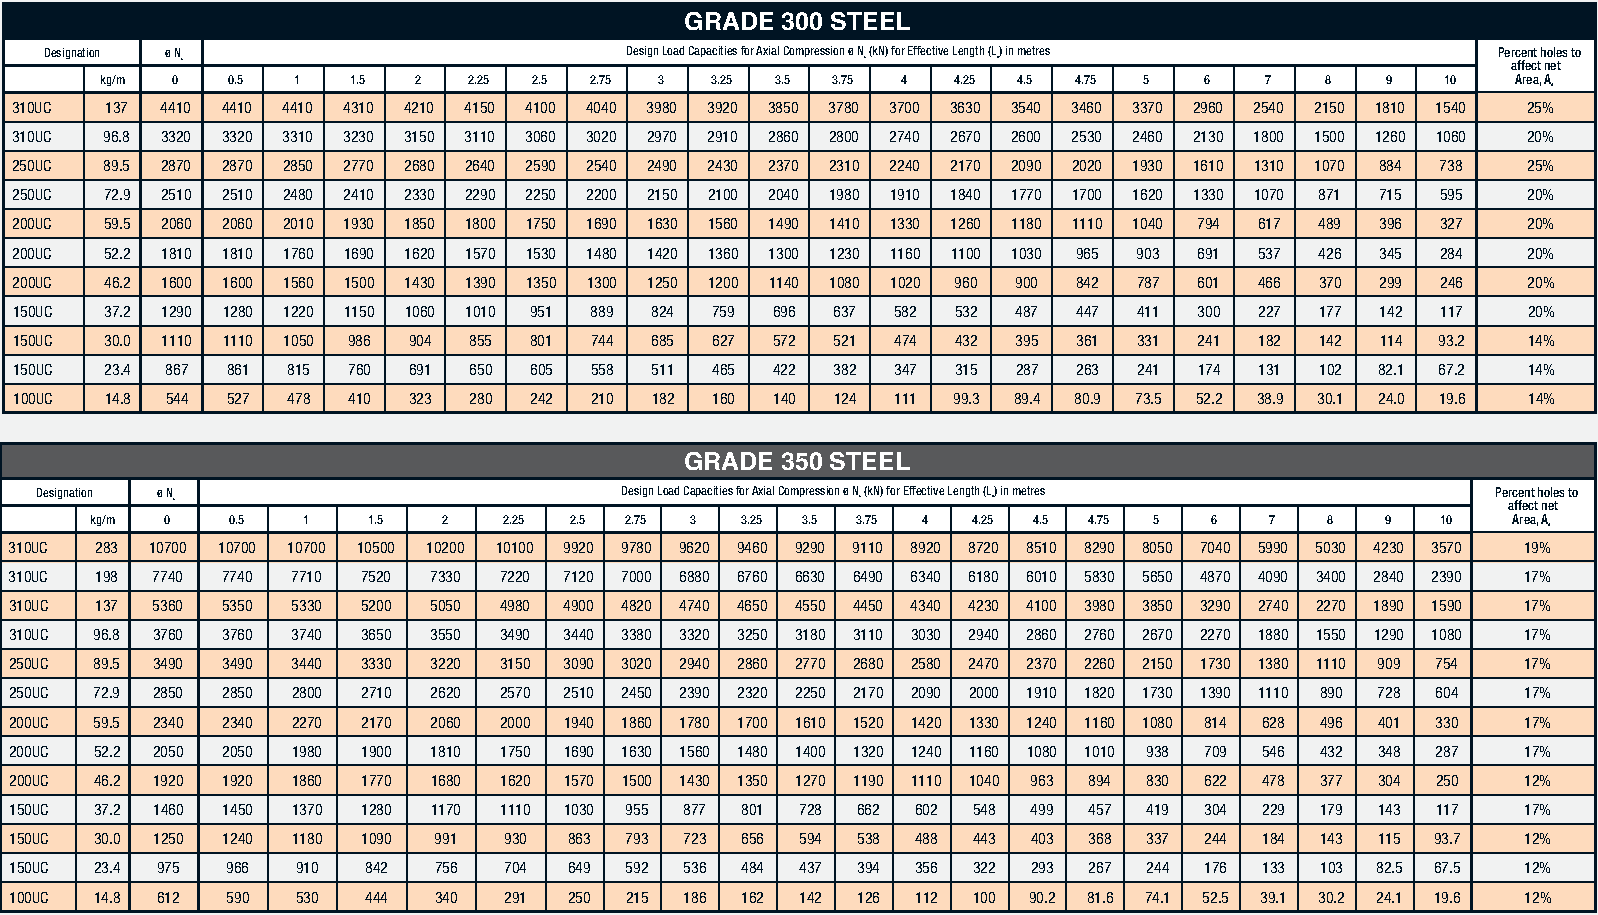
\includegraphics[width=\linewidth]{PIC/CH04/TABLE}
\caption{Design load capacity table for members subject to axial compression buckling about weak axis}\label{fig:design_table}
\end{sidewaysfigure}
\begin{sidewaysfigure}[p]
\centering
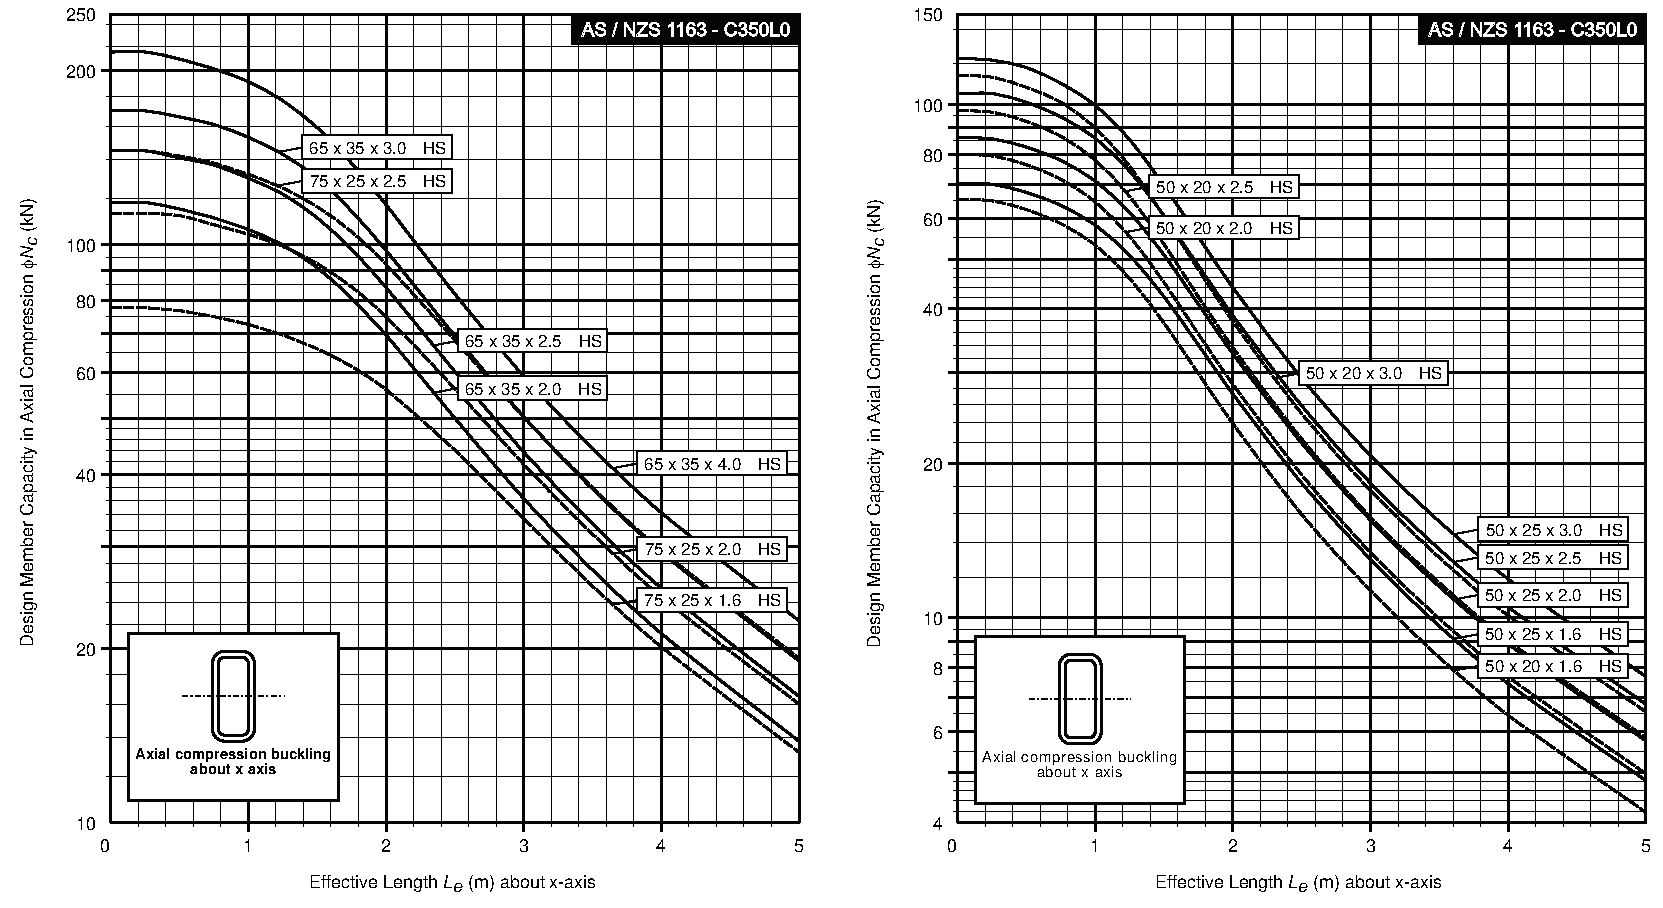
\includegraphics[width=\linewidth]{PIC/CH04/CHART}
\caption{Design capacity chart for members subject to axial compression}\label{fig:design_chart}
\end{sidewaysfigure}
\begin{sidewaystable}[p]
\centering\scriptsize\setlength{\tabcolsep}{2pt}\renewcommand{\arraystretch}{1.4}
\caption{Design load capacity table for UB members subject to axial compression buckling about strong axis (manually generated)}\label{tab:ub_strong}
\begin{tabular}{r|c|ccccccccccccccccccccccccc}
	\toprule
	                                                                                        \multicolumn{27}{c}{\Large{}Grade 300 Steel UB Section Subject to Axial Compression \textbf{Strong} Axis Buckling}                                                                                         \\ \midrule
	                    & \multicolumn{1}{c|}{$\phi{}N_s$ (\si{\kn})} &                                                                                          \multicolumn{25}{c}{$\phi{}N_c$ (\si{\kn})}                                                                                           \\
	$L_e$ (\si{\meter}) &                      0                      &   2    &  2.5   &   3    &  3.5   &   4    &  4.5   &   5    &  5.5   &   6    &  6.5   &   7    &  7.5   &   8    &  8.5   &   9    &  9.5   &   10   &   11   &   12   &   13   &   14   &   15   &   16   &   17   &   18   \\ \midrule
	           610UB125 &                   3830.4                    & 3830.4 & 3830.4 & 3830.4 & 3817.6 & 3791.1 & 3764.5 & 3737.7 & 3710.7 & 3683.3 & 3655.5 & 3627.2 & 3598.3 & 3568.8 & 3538.7 & 3507.7 & 3475.9 & 3443.2 & 3374.7 & 3301.6 & 3223.5 & 3139.9 & 3050.6 & 2955.7 & 2855.5 & 2750.5 \\
	                113 &                   3383.6                    & 3383.6 & 3383.6 & 3383.6 & 3372.4 & 3349.0 & 3325.6 & 3301.9 & 3278.0 & 3253.8 & 3229.3 & 3204.3 & 3178.9 & 3152.8 & 3126.2 & 3098.9 & 3070.8 & 3042.0 & 2981.5 & 2917.0 & 2848.1 & 2774.4 & 2695.6 & 2611.9 & 2523.5 & 2430.9 \\
	                101 &                   3116.9                    & 3116.9 & 3116.9 & 3116.9 & 3102.0 & 3079.8 & 3057.5 & 3034.9 & 3012.2 & 2989.1 & 2965.7 & 2941.8 & 2917.4 & 2892.5 & 2866.9 & 2840.6 & 2813.5 & 2785.6 & 2727.0 & 2664.4 & 2597.3 & 2525.4 & 2448.5 & 2366.9 & 2280.9 & 2191.2 \\
	          530UB92.4 &                   2956.6                    & 2956.6 & 2956.6 & 2945.9 & 2921.8 & 2897.7 & 2873.3 & 2848.6 & 2823.5 & 2797.8 & 2771.6 & 2744.7 & 2717.0 & 2688.4 & 2658.8 & 2628.2 & 2596.5 & 2563.5 & 2493.5 & 2417.8 & 2336.0 & 2248.3 & 2155.2 & 2057.6 & 1957.0 & 1855.1 \\
	               82.0 &                   2557.2                    & 2557.2 & 2557.2 & 2547.3 & 2526.5 & 2505.5 & 2484.3 & 2462.8 & 2440.9 & 2418.6 & 2395.8 & 2372.4 & 2348.3 & 2323.4 & 2297.7 & 2271.0 & 2243.4 & 2214.6 & 2153.6 & 2087.6 & 2016.2 & 1939.7 & 1858.6 & 1773.6 & 1686.1 & 1597.5 \\
	          460UB82.1 &                   2775.5                    & 2775.5 & 2767.0 & 2740.3 & 2713.3 & 2686.1 & 2658.3 & 2629.9 & 2600.8 & 2570.7 & 2539.6 & 2507.2 & 2473.5 & 2438.4 & 2401.6 & 2363.0 & 2322.6 & 2280.3 & 2189.7 & 2091.2 & 1985.8 & 1875.4 & 1762.2 & 1649.1 & 1538.4 & 1432.3 \\
	               74.6 &                   2436.7                    & 2436.7 & 2431.2 & 2408.1 & 2384.8 & 2361.3 & 2337.4 & 2313.0 & 2287.9 & 2262.1 & 2235.4 & 2207.7 & 2178.9 & 2148.8 & 2117.4 & 2084.5 & 2050.1 & 2014.1 & 1936.9 & 1853.0 & 1763.1 & 1668.4 & 1571.0 & 1473.0 & 1376.7 & 1283.8 \\
	               67.1 &                   2135.9                    & 2135.9 & 2131.4 & 2111.2 & 2090.9 & 2070.3 & 2049.4 & 2028.1 & 2006.2 & 1983.7 & 1960.4 & 1936.2 & 1911.1 & 1884.9 & 1857.5 & 1828.9 & 1798.9 & 1767.5 & 1700.3 & 1627.2 & 1548.8 & 1466.3 & 1381.2 & 1295.6 & 1211.3 & 1129.9 \\
	          410UB59.7 &                   1934.9                    & 1934.9 & 1920.1 & 1899.6 & 1878.9 & 1857.8 & 1836.3 & 1814.1 & 1791.1 & 1767.2 & 1742.4 & 1716.3 & 1689.0 & 1660.3 & 1630.0 & 1598.2 & 1564.7 & 1529.6 & 1454.4 & 1373.5 & 1288.6 & 1202.0 & 1116.1 & 1033.2 & 954.6  & 881.5  \\
	               53.7 &                   1811.7                    & 1811.7 & 1794.3 & 1774.3 & 1754.1 & 1733.5 & 1712.4 & 1690.6 & 1667.9 & 1644.4 & 1619.7 & 1593.8 & 1566.5 & 1537.7 & 1507.4 & 1475.5 & 1441.8 & 1406.5 & 1331.1 & 1250.6 & 1167.1 & 1083.1 & 1001.0 & 922.7  & 849.6  & 782.2  \\
	          360UB56.7 &                   1947.0                    & 1939.4 & 1915.4 & 1891.3 & 1866.6 & 1841.2 & 1814.9 & 1787.5 & 1758.8 & 1728.6 & 1696.6 & 1662.7 & 1626.7 & 1588.5 & 1548.1 & 1505.3 & 1460.5 & 1413.7 & 1315.6 & 1214.5 & 1114.2 & 1018.1 & 928.4  & 846.3  & 772.1  & 705.5  \\
	               50.7 &                   1682.3                    & 1676.5 & 1656.1 & 1635.4 & 1614.3 & 1592.7 & 1570.3 & 1546.9 & 1522.5 & 1496.8 & 1469.6 & 1440.9 & 1410.3 & 1378.0 & 1343.7 & 1307.5 & 1269.5 & 1229.7 & 1146.3 & 1060.0 & 973.9  & 891.1  & 813.5  & 742.2  & 677.6  & 619.5  \\
	               44.7 &                   1532.0                    & 1524.7 & 1505.5 & 1486.1 & 1466.2 & 1445.8 & 1424.6 & 1402.5 & 1379.3 & 1354.7 & 1328.8 & 1301.2 & 1271.9 & 1240.7 & 1207.8 & 1173.0 & 1136.5 & 1098.4 & 1019.2 & 938.0  & 858.2  & 782.3  & 712.0  & 648.0  & 590.4  & 539.0  \\
	          310UB46.2 &                   1586.7                    & 1569.3 & 1546.9 & 1524.0 & 1500.4 & 1475.9 & 1450.1 & 1422.9 & 1393.9 & 1362.9 & 1329.8 & 1294.4 & 1256.5 & 1216.3 & 1173.8 & 1129.4 & 1083.5 & 1036.6 & 942.4  & 851.2  & 766.3  & 689.3  & 620.7  & 560.2  & 507.1  & 460.4  \\
	               40.4 &                   1428.5                    & 1411.2 & 1390.6 & 1369.5 & 1347.7 & 1325.0 & 1301.2 & 1275.8 & 1248.9 & 1220.0 & 1189.1 & 1155.9 & 1120.5 & 1082.9 & 1043.2 & 1001.9 & 959.4  & 916.2  & 829.9  & 747.3  & 671.0  & 602.4  & 541.7  & 488.3  & 441.5  & 400.6  \\
	               32.0 &                   1075.2                    & 1061.0 & 1045.1 & 1028.9 & 1012.1 & 994.5  & 976.0  & 956.4  & 935.4  & 912.8  & 888.7  & 862.8  & 835.1  & 805.7  & 774.8  & 742.7  & 709.8  & 676.6  & 610.7  & 548.3  & 491.1  & 440.1  & 395.1  & 355.8  & 321.4  & 291.4  \\
	          250UB37.3 &                   1368.0                    & 1333.8 & 1309.1 & 1283.3 & 1256.1 & 1227.0 & 1195.5 & 1161.4 & 1124.2 & 1083.8 & 1040.2 & 993.7  & 944.9  & 894.5  & 843.7  & 793.4  & 744.4  & 697.4  & 611.1  & 536.0  & 471.7  & 417.1  & 370.7  & 331.1  & 297.3  & 268.3  \\
	               31.4 &                   1154.9                    & 1123.7 & 1102.1 & 1079.5 & 1055.6 & 1029.9 & 1002.1 & 971.8  & 938.6  & 902.6  & 863.8  & 822.6  & 779.6  & 735.6  & 691.5  & 648.3  & 606.6  & 567.0  & 494.9  & 432.9  & 380.2  & 335.7  & 298.0  & 266.0  & 238.6  & 215.2  \\
	               25.7 &                    893.7                    & 870.6  & 854.3  & 837.2  & 819.1  & 799.8  & 778.8  & 756.0  & 731.2  & 704.2  & 675.1  & 644.1  & 611.6  & 578.2  & 544.7  & 511.5  & 479.4  & 448.7  & 392.5  & 343.9  & 302.4  & 267.2  & 237.4  & 212.0  & 190.3  & 171.6  \\
	          200UB29.8 &                   1100.2                    & 1053.8 & 1028.1 & 1000.5 & 970.3  & 936.9  & 899.9  & 858.9  & 814.0  & 766.0  & 716.0  & 665.5  & 615.9  & 568.5  & 524.0  & 482.8  & 445.1  & 410.9  & 351.8  & 303.5  & 263.9  & 231.3  & 204.1  & 181.4  & 162.2  & 145.8  \\
	               25.4 &                    930.2                    & 889.2  & 866.8  & 842.7  & 816.2  & 786.9  & 754.2  & 718.1  & 678.6  & 636.5  & 593.1  & 549.5  & 507.2  & 467.0  & 429.5  & 395.1  & 363.8  & 335.4  & 286.7  & 247.0  & 214.6  & 187.9  & 165.8  & 147.3  & 131.7  & 118.3  \\
	               22.3 &                    826.6                    & 790.2  & 770.3  & 748.9  & 725.5  & 699.4  & 670.5  & 638.4  & 603.4  & 566.1  & 527.6  & 488.9  & 451.3  & 415.6  & 382.3  & 351.7  & 323.8  & 298.6  & 255.2  & 219.9  & 191.1  & 167.4  & 147.7  & 131.2  & 117.2  & 105.4  \\
	               18.2 &                    661.5                    & 630.5  & 614.0  & 596.1  & 576.4  & 554.4  & 529.9  & 502.8  & 473.3  & 442.0  & 410.1  & 378.5  & 348.1  & 319.6  & 293.2  & 269.2  & 247.4  & 227.8  & 194.3  & 167.2  & 145.1  & 127.0  & 112.0  &  99.4  &  88.8  &  79.8  \\
	          180UB22.2 &                    812.2                    & 763.9  & 740.0  & 713.5  & 683.7  & 649.9  & 612.0  & 570.5  & 526.8  & 482.6  & 439.7  & 399.5  & 362.5  & 329.2  & 299.4  & 272.9  & 249.4  & 228.6  & 193.6  & 165.7  & 143.3  & 125.0  & 110.0  &  97.5  &  87.0  &  78.1  \\
	               18.1 &                    662.4                    & 622.0  & 602.2  & 580.1  & 555.1  & 526.8  & 495.1  & 460.5  & 424.2  & 387.7  & 352.6  & 319.8  & 289.8  & 262.9  & 238.9  & 217.6  & 198.8  & 182.1  & 154.1  & 131.9  & 114.0  &  99.4  &  87.5  &  77.5  &  69.1  &  62.1  \\
	               16.1 &                    587.5                    & 551.1  & 533.3  & 513.5  & 491.0  & 465.5  & 436.9  & 405.8  & 373.3  & 340.7  & 309.5  & 280.4  & 253.9  & 230.2  & 209.1  & 190.4  & 173.8  & 159.2  & 134.7  & 115.2  &  99.6  &  86.9  &  76.4  &  67.7  &  60.4  &  54.2  \\
	          150UB18.0 &                    662.4                    & 609.9  & 585.1  & 556.8  & 524.0  & 486.7  & 445.9  & 403.7  & 362.4  & 323.8  & 289.0  & 258.2  & 231.4  & 208.0  & 187.6  & 170.0  & 154.5  & 141.0  & 118.7  & 101.1  &  87.2  &  75.9  &  66.6  &  58.9  &  52.5  &  47.1  \\
	               14.0 &                    512.6                    & 470.0  & 450.0  & 426.9  & 400.2  & 369.8  & 337.0  & 303.4  & 271.0  & 241.3  & 214.7  & 191.4  & 171.2  & 153.7  & 138.5  & 125.4  & 113.9  & 103.9  &  87.3  &  74.4  &  64.1  &  55.7  &  48.9  &  43.3  &  38.6  &  34.6  \\ \bottomrule
\end{tabular}
\end{sidewaystable}
\begin{sidewaystable}[p]
\centering\scriptsize\setlength{\tabcolsep}{2pt}\renewcommand{\arraystretch}{1.4}
\caption{Design load capacity table for UB members subject to axial compression buckling about weak axis (manually generated)}\label{tab:ub_weak}
\begin{tabular}{r|c|ccccccccccccccccccccccccc}
	\toprule
	                                                                                        \multicolumn{27}{c}{\Large{}Grade 300 Steel UB Section Subject to Axial Compression \textbf{Weak} Axis Buckling}                                                                                         \\ \midrule
	                    & \multicolumn{1}{c|}{$\phi{}N_s$ (\si{\kn})} &                                                                                         \multicolumn{25}{c}{$\phi{}N_c$ (\si{\kn})}                                                                                          \\
	$L_e$ (\si{\meter}) &                      0                      &   2    &  2.25  &  2.5   &  2.75  &   3    &  3.25  &  3.5   &  3.75  &   4    &  4.25  &  4.5   &  4.75  &   5    &  5.25  &  5.5   &  5.75  &   6    &  6.25  &  6.5   &  6.75  &   7    &  7.25  &  7.5   & 7.75  &   8   \\ \midrule
	           610UB125 &                   3830.4                    & 3440.5 & 3353.6 & 3259.2 & 3156.6 & 3045.1 & 2924.7 & 2796.1 & 2661.0 & 2521.5 & 2380.2 & 2240.0 & 2103.2 & 1971.7 & 1846.8 & 1729.5 & 1619.9 & 1518.1 & 1423.9 & 1336.9 & 1256.6 & 1182.5 & 1114.3 & 1051.3 & 993.1 & 939.4 \\
	                113 &                   3383.6                    & 3035.9 & 2958.4 & 2874.3 & 2782.6 & 2683.1 & 2575.6 & 2460.9 & 2340.5 & 2216.3 & 2090.9 & 1966.5 & 1845.4 & 1729.2 & 1619.0 & 1515.6 & 1419.1 & 1329.6 & 1246.8 & 1170.4 & 1099.9 & 1034.9 & 975.1  & 919.8  & 868.9 & 821.8 \\
	                101 &                   3116.9                    & 2774.8 & 2698.6 & 2615.4 & 2524.6 & 2425.8 & 2319.4 & 2206.5 & 2089.0 & 1969.1 & 1849.4 & 1732.3 & 1619.6 & 1512.7 & 1412.4 & 1319.0 & 1232.5 & 1152.8 & 1079.4 & 1011.9 & 949.9  & 893.0  & 840.6  & 792.4  & 748.1 & 707.1 \\
	          530UB92.4 &                   2956.6                    & 2585.7 & 2502.7 & 2411.3 & 2311.2 & 2202.5 & 2086.6 & 1965.6 & 1842.5 & 1720.2 & 1601.5 & 1488.3 & 1382.0 & 1283.3 & 1192.2 & 1108.7 & 1032.3 & 962.6  & 899.0  & 841.0  & 788.0  & 739.5  & 695.2  & 654.5  & 617.1 & 582.8 \\
	               82.0 &                   2557.2                    & 2230.5 & 2157.3 & 2076.7 & 1988.3 & 1892.4 & 1790.4 & 1684.2 & 1576.6 & 1470.0 & 1367.0 & 1269.1 & 1177.5 & 1092.6 & 1014.4 & 942.9  & 877.6  & 818.0  & 763.7  & 714.2  & 669.1  & 627.8  & 590.0  & 555.4  & 523.7 & 494.5 \\
	          460UB82.1 &                   2775.5                    & 2370.1 & 2278.2 & 2176.6 & 2065.3 & 1946.0 & 1821.4 & 1695.0 & 1570.6 & 1451.0 & 1338.6 & 1234.3 & 1138.7 & 1051.6 & 972.6  & 901.0  & 836.3  & 777.7  & 724.7  & 676.5  & 632.8  & 593.0  & 556.7  & 523.6  & 493.2 & 465.3 \\
	               74.6 &                   2436.7                    & 2084.8 & 2005.2 & 1917.0 & 1820.6 & 1716.9 & 1608.5 & 1498.3 & 1389.5 & 1284.7 & 1185.9 & 1094.1 & 1009.8 & 932.9  & 863.0  & 799.7  & 742.4  & 690.5  & 643.5  & 600.9  & 562.1  & 526.8  & 494.6  & 465.2  & 438.2 & 413.5 \\
	               67.1 &                   2135.9                    & 1827.2 & 1757.3 & 1679.9 & 1595.3 & 1504.3 & 1409.2 & 1312.6 & 1217.1 & 1125.3 & 1038.7 & 958.2  & 884.4  & 817.0  & 755.8  & 700.3  & 650.2  & 604.7  & 563.5  & 526.2  & 492.2  & 461.3  & 433.1  & 407.4  & 383.8 & 362.1 \\
	          410UB59.7 &                   1934.9                    & 1632.3 & 1563.2 & 1486.8 & 1403.4 & 1314.8 & 1223.4 & 1132.2 & 1043.8 & 960.2  & 882.5  & 811.4  & 746.6  & 688.1  & 635.3  & 587.7  & 544.9  & 506.2  & 471.3  & 439.7  & 411.0  & 384.9  & 361.2  & 339.5  & 319.7 & 301.6 \\
	               53.7 &                   1811.7                    & 1504.4 & 1433.6 & 1355.4 & 1270.7 & 1181.9 & 1092.0 & 1004.1 & 920.5  & 842.7  & 771.5  & 707.0  & 648.9  & 596.8  & 550.0  & 508.1  & 470.4  & 436.6  & 406.1  & 378.6  & 353.6  & 331.0  & 310.5  & 291.7  & 274.6 & 258.9 \\
	          360UB56.7 &                   1947.0                    & 1616.2 & 1540.0 & 1455.8 & 1364.6 & 1269.1 & 1172.4 & 1077.9 & 988.0  & 904.5  & 828.0  & 758.7  & 696.3  & 640.3  & 590.1  & 545.1  & 504.7  & 468.4  & 435.7  & 406.2  & 379.4  & 355.1  & 333.1  & 313.0  & 294.6 & 277.7 \\
	               50.7 &                   1682.3                    & 1398.4 & 1333.1 & 1260.8 & 1182.6 & 1100.5 & 1017.3 & 935.7  & 858.1  & 785.8  & 719.6  & 659.6  & 605.5  & 556.9  & 513.3  & 474.2  & 439.1  & 407.6  & 379.1  & 353.4  & 330.2  & 309.1  & 289.9  & 272.4  & 256.4 & 241.7 \\
	               44.7 &                   1532.0                    & 1255.5 & 1191.5 & 1120.9 & 1045.0 & 966.5  & 888.2  & 812.8  & 742.1  & 677.2  & 618.3  & 565.3  & 518.0  & 475.7  & 437.9  & 404.1  & 373.8  & 346.7  & 322.3  & 300.3  & 280.4  & 262.4  & 246.0  & 231.0  & 217.4 & 204.9 \\
	          310UB46.2 &                   1586.7                    & 1318.3 & 1256.5 & 1188.2 & 1114.2 & 1036.6 & 958.0  & 881.1  & 807.8  & 739.7  & 677.3  & 620.7  & 569.8  & 524.0  & 483.0  & 446.2  & 413.1  & 383.4  & 356.7  & 332.5  & 310.6  & 290.8  & 272.7  & 256.2  & 241.2 & 227.4 \\
	               40.4 &                   1428.5                    & 1173.7 & 1114.7 & 1049.7 & 979.7  & 907.1  & 834.5  & 764.3  & 698.4  & 637.6  & 582.5  & 532.8  & 488.3  & 448.5  & 413.0  & 381.2  & 352.7  & 327.2  & 304.2  & 283.4  & 264.7  & 247.7  & 232.2  & 218.1  & 205.3 & 193.5 \\
	               32.0 &                   1075.2                    & 832.9  & 776.1  & 715.0  & 652.3  & 591.1  & 533.5  & 480.9  & 433.7  & 392.0  & 355.1  & 322.7  & 294.2  & 269.1  & 246.8  & 227.2  & 209.7  & 194.1  & 180.1  & 167.5  & 156.2  & 146.0  & 136.8  & 128.3  & 120.7 & 113.7 \\
	          250UB37.3 &                   1368.0                    & 1061.4 & 989.5  & 912.1  & 832.7  & 754.9  & 681.6  & 614.6  & 554.5  & 501.2  & 454.1  & 412.7  & 376.3  & 344.2  & 315.8  & 290.6  & 268.3  & 248.3  & 230.4  & 214.4  & 199.9  & 186.9  & 175.0  & 164.2  & 154.4 & 145.5 \\
	               31.4 &                   1154.9                    & 880.7  & 816.4  & 748.0  & 678.8  & 612.2  & 550.5  & 494.7  & 445.2  & 401.5  & 363.3  & 329.7  & 300.3  & 274.5  & 251.6  & 231.5  & 213.5  & 197.6  & 183.3  & 170.5  & 158.9  & 148.5  & 139.0  & 130.5  & 122.6 & 115.5 \\
	               25.7 &                    893.7                    & 614.6  & 552.2  & 490.9  & 433.9  & 383.1  & 338.8  & 300.6  & 267.9  & 239.8  & 215.7  & 194.9  & 176.8  & 161.1  & 147.3  & 135.2  & 124.5  & 115.0  & 106.5  &  99.0  &  92.2  &  86.0  &  80.5  &  75.5  & 70.9  & 66.7  \\
	          200UB29.8 &                   1100.2                    & 814.9  & 748.5  & 679.3  & 611.1  & 547.1  & 489.0  & 437.4  & 392.2  & 352.8  & 318.5  & 288.6  & 262.5  & 239.6  & 219.5  & 201.7  & 186.0  & 171.9  & 159.4  & 148.2  & 138.1  & 129.0  & 120.8  & 113.3  & 106.5 & 100.3 \\
	               25.4 &                    930.2                    & 674.9  & 615.9  & 555.4  & 496.9  & 442.8  & 394.4  & 351.8  & 314.8  & 282.7  & 254.9  & 230.8  & 209.7  & 191.3  & 175.1  & 160.9  & 148.3  & 137.0  & 127.0  & 118.1  & 110.0  & 102.7  &  96.1  &  90.2  & 84.7  & 79.8  \\
	               22.3 &                    826.6                    & 602.3  & 550.4  & 497.0  & 445.1  & 397.0  & 353.8  & 315.8  & 282.7  & 254.0  & 229.0  & 207.4  & 188.5  & 172.0  & 157.5  & 144.7  & 133.3  & 123.2  & 114.2  & 106.2  &  98.9  &  92.4  &  86.5  &  81.1  & 76.2  & 71.8  \\
	               18.2 &                    661.5                    & 349.6  & 297.8  & 254.0  & 217.8  & 188.1  & 163.7  & 143.5  & 126.7  & 112.6  & 100.7  &  90.6  &  81.9  &  74.4  &  67.8  &  62.1  &  57.1  &  52.6  &  48.7  &  45.2  &  42.0  &  39.2  &  36.6  &  34.3  & 32.2  & 30.3  \\
	          180UB22.2 &                    812.2                    & 393.5  & 331.6  & 280.7  & 239.5  & 206.1  & 178.9  & 156.5  & 138.0  & 122.5  & 109.5  &  98.4  &  88.9  &  80.7  &  73.5  &  67.3  &  61.8  &  57.0  &  52.7  &  48.9  &  45.5  &  42.4  &  39.6  &  37.1  & 34.8  & 32.7  \\
	               18.1 &                    662.4                    & 316.7  & 266.5  & 225.4  & 192.1  & 165.2  & 143.4  & 125.4  & 110.6  &  98.2  &  87.7  &  78.8  &  71.2  &  64.6  &  58.9  &  53.9  &  49.5  &  45.6  &  42.2  &  39.1  &  36.4  &  33.9  &  31.7  &  29.7  & 27.9  & 26.2  \\
	               16.1 &                    587.5                    & 277.1  & 232.8  & 196.7  & 167.6  & 144.1  & 125.0  & 109.3  &  96.3  &  85.5  &  76.4  &  68.6  &  62.0  &  56.3  &  51.3  &  46.9  &  43.1  &  39.7  &  36.7  &  34.1  &  31.7  &  29.5  &  27.6  &  25.8  & 24.3  & 22.8  \\
	          150UB18.0 &                    662.4                    & 239.3  & 196.9  & 164.1  & 138.5  & 118.3  & 102.1  &  89.0  &  78.2  &  69.3  &  61.8  &  55.4  &  50.0  &  45.3  &  41.3  &  37.7  &  34.6  &  31.9  &  29.5  &  27.3  &  25.4  &  23.7  &  22.1  &  20.7  & 19.4  & 18.2  \\
	               14.0 &                    512.6                    & 176.5  & 144.9  & 120.5  & 101.6  &  86.7  &  74.8  &  65.2  &  57.3  &  50.7  &  45.2  &  40.5  &  36.5  &  33.1  &  30.2  &  27.6  &  25.3  &  23.3  &  21.5  &  20.0  &  18.5  &  17.3  &  16.1  &  15.1  & 14.2  & 13.3  \\ \bottomrule
\end{tabular}
\end{sidewaystable}
\begin{sidewaystable}[p]
\centering\scriptsize\setlength{\tabcolsep}{2pt}\renewcommand{\arraystretch}{1.2}
\caption{Design load capacity table for UC members subject to axial compression buckling about strong axis (manually generated)}\label{tab:uc_strong}
\begin{tabular}{r|c|ccccccccccccccccccccccccc}
	\toprule
	                                                                             \multicolumn{27}{c}{\Large{}Grade 300 Steel UC Section Subject to Axial Compression \textbf{Strong}  Axis Buckling}                                                                              \\ \midrule
	                    & $\phi{}N_s$ (\si{\kn}) &                                                                                          \multicolumn{25}{c}{$\phi{}N_c$ (\si{\kn})}                                                                                           \\
	$L_e$ (\si{\meter}) &           0            &   2    &  2.5   &   3    &  3.5   &   4    &  4.5   &   5    &  5.5   &   6    &  6.5   &   7    &  7.5   &   8    &  8.5   &   9    &  9.5   &   10   &   11   &   12   &   13   &   14   &   15   &   16   &   17   &   18   \\ \midrule
	           310UC158 &         5065.2         & 5036.0 & 4971.4 & 4905.9 & 4838.8 & 4769.7 & 4697.9 & 4622.7 & 4543.6 & 4460.0 & 4371.3 & 4276.9 & 4176.6 & 4069.9 & 3956.9 & 3837.7 & 3712.9 & 3583.2 & 3314.1 & 3040.9 & 2774.5 & 2523.3 & 2292.1 & 2082.9 & 1895.5 & 1728.6 \\
	                137 &         4410.0         & 4381.3 & 4324.2 & 4266.2 & 4206.9 & 4145.6 & 4081.8 & 4014.9 & 3944.5 & 3869.9 & 3790.6 & 3706.3 & 3616.4 & 3520.9 & 3419.8 & 3313.2 & 3201.7 & 3086.1 & 2847.2 & 2606.2 & 2372.9 & 2154.2 & 1954.1 & 1773.7 & 1612.7 & 1469.6 \\
	                118 &         3780.0         & 3754.0 & 3704.6 & 3654.5 & 3603.2 & 3550.2 & 3494.9 & 3437.0 & 3375.9 & 3311.2 & 3242.4 & 3169.1 & 3091.0 & 3008.0 & 2920.1 & 2827.4 & 2730.7 & 2630.4 & 2423.7 & 2215.9 & 2015.4 & 1828.0 & 1657.0 & 1503.2 & 1366.1 & 1244.5 \\
	               96.8 &         3348.0         & 3316.1 & 3270.1 & 3223.2 & 3175.0 & 3124.9 & 3072.5 & 3017.3 & 2958.7 & 2896.3 & 2829.6 & 2758.4 & 2682.4 & 2601.6 & 2516.1 & 2426.4 & 2333.4 & 2237.9 & 2044.0 & 1853.8 & 1674.5 & 1510.4 & 1363.0 & 1232.1 & 1116.7 & 1015.0 \\
	          250UC89.5 &         2872.8         & 2820.9 & 2774.7 & 2727.1 & 2677.4 & 2624.9 & 2569.1 & 2509.2 & 2444.7 & 2375.1 & 2299.9 & 2219.2 & 2133.3 & 2042.9 & 1949.1 & 1853.3 & 1757.1 & 1661.9 & 1479.5 & 1313.4 & 1166.4 & 1038.3 & 927.5  & 831.8  & 749.2  & 677.6  \\
	               72.9 &         2516.4         & 2463.8 & 2421.3 & 2377.4 & 2331.2 & 2282.3 & 2229.9 & 2173.4 & 2112.2 & 2045.9 & 1974.4 & 1897.6 & 1816.3 & 1731.3 & 1644.0 & 1556.0 & 1468.6 & 1383.3 & 1222.9 & 1079.7 & 954.9  & 847.4  & 755.2  & 676.1  & 608.1  & 549.4  \\
	          200UC59.5 &         2057.4         & 1981.4 & 1936.8 & 1889.3 & 1838.0 & 1781.7 & 1719.8 & 1651.3 & 1576.3 & 1495.2 & 1409.4 & 1320.8 & 1231.9 & 1144.8 & 1061.4 & 982.9  & 910.0  & 842.8  & 725.4  & 628.1  & 547.6  & 480.8  & 425.1  & 378.2  & 338.5  & 304.6  \\
	               52.2 &         1798.2         & 1730.8 & 1691.4 & 1649.6 & 1604.2 & 1554.5 & 1499.6 & 1439.1 & 1372.6 & 1300.9 & 1225.1 & 1147.1 & 1068.9 & 992.5  & 919.6  & 851.1  & 787.5  & 729.1  & 627.1  & 542.8  & 473.1  & 415.3  & 367.1  & 326.5  & 292.2  & 262.9  \\
	               46.2 &         1593.0         & 1531.9 & 1496.6 & 1459.0 & 1418.1 & 1373.3 & 1323.8 & 1269.1 & 1209.1 & 1144.4 & 1076.2 & 1006.2 & 936.4  & 868.5  & 803.8  & 743.3  & 687.3  & 635.9  & 546.4  & 472.6  & 411.7  & 361.3  & 319.3  & 284.0  & 254.1  & 228.6  \\
	          150UC37.2 &         1277.1         & 1195.2 & 1155.3 & 1110.8 & 1060.2 & 1002.7 & 938.3  & 868.6  & 796.3  & 724.6  & 656.4  & 593.4  & 536.5  & 485.7  & 440.7  & 400.9  & 365.8  & 334.8  & 283.0  & 241.9  & 209.0  & 182.2  & 160.2  & 142.0  & 126.6  & 113.6  \\
	               30.0 &         1111.7         & 1034.2 & 997.1  & 955.2  & 907.2  & 852.6  & 791.8  & 726.9  & 661.0  & 597.1  & 537.6  & 483.6  & 435.5  & 393.1  & 355.8  & 323.1  & 294.4  & 269.1  & 227.0  & 193.8  & 167.3  & 145.7  & 128.1  & 113.4  & 101.1  &  90.7  \\
	               23.4 &         858.2          & 794.4  & 764.1  & 729.6  & 690.0  & 644.8  & 594.9  & 542.4  & 490.0  & 440.2  & 394.5  & 353.7  & 317.6  & 286.1  & 258.5  & 234.4  & 213.3  & 194.8  & 164.2  & 140.0  & 120.8  & 105.1  &  92.4  &  81.7  &  72.9  &  65.3  \\
	          100UC14.8 &         544.3          & 454.7  & 411.4  & 360.6  & 307.9  & 259.4  & 218.2  & 184.5  & 157.2  & 135.2  & 117.3  & 102.6  &  90.5  &  80.3  &  71.7  &  64.5  &  58.2  &  52.8  &  44.1  &  37.3  &  32.0  &  27.8  &  24.3  &  21.4  &  19.1  &  17.0  \\ \bottomrule
\end{tabular}
\caption{Design load capacity table for UC members subject to axial compression buckling about weak axis (manually generated)}\label{tab:uc_weak}
\begin{tabular}{r|c|ccccccccccccccccccccccccc}
	\toprule
	                                                                              \multicolumn{27}{c}{\Large{}Grade 300 Steel UC Section Subject to Axial Compression \textbf{Weak} Axis Buckling}                                                                                \\ \midrule
	                    & $\phi{}N_s$ (\si{\kn}) &                                                                                          \multicolumn{25}{c}{$\phi{}N_c$ (\si{\kn})}                                                                                           \\
	$L_e$ (\si{\meter}) &           0            &   2    &  2.25  &  2.5   &  2.75  &   3    &  3.25  &  3.5   &  3.75  &   4    &  4.25  &  4.5   &  4.75  &   5    &  5.25  &  5.5   &  5.75  &   6    &  6.25  &  6.5   &  6.75  &   7    &  7.25  &  7.5   &  7.75  &   8    \\ \midrule
	           310UC158 &         5065.2         & 4835.6 & 4774.8 & 4711.9 & 4646.4 & 4578.1 & 4506.5 & 4431.1 & 4351.7 & 4267.8 & 4179.2 & 4085.7 & 3987.3 & 3884.0 & 3776.2 & 3664.3 & 3548.9 & 3430.9 & 3311.1 & 3190.6 & 3070.4 & 2951.2 & 2834.0 & 2719.5 & 2608.3 & 2500.7 \\
	                137 &         4410.0         & 4206.4 & 4152.8 & 4097.4 & 4039.7 & 3979.4 & 3916.1 & 3849.5 & 3779.2 & 3704.9 & 3626.5 & 3543.7 & 3456.5 & 3365.1 & 3269.7 & 3170.7 & 3068.9 & 2964.8 & 2859.4 & 2753.5 & 2648.0 & 2543.7 & 2441.3 & 2341.4 & 2244.5 & 2151.0 \\
	                118 &         3780.0         & 3602.2 & 3555.7 & 3507.6 & 3457.5 & 3405.1 & 3350.1 & 3292.1 & 3230.9 & 3166.2 & 3097.8 & 3025.5 & 2949.5 & 2869.8 & 2786.7 & 2700.6 & 2612.0 & 2521.7 & 2430.4 & 2338.9 & 2247.8 & 2157.9 & 2069.9 & 1984.2 & 1901.1 & 1821.1 \\
	               96.8 &         3348.0         & 3175.6 & 3132.0 & 3086.6 & 3039.2 & 2989.4 & 2936.9 & 2881.4 & 2822.5 & 2760.2 & 2694.1 & 2624.4 & 2551.1 & 2474.4 & 2394.8 & 2312.8 & 2229.1 & 2144.4 & 2059.6 & 1975.4 & 1892.5 & 1811.5 & 1732.8 & 1656.8 & 1583.9 & 1514.0 \\
	          250UC89.5 &         2872.8         & 2683.9 & 2639.4 & 2592.5 & 2542.8 & 2490.0 & 2433.6 & 2373.3 & 2309.0 & 2240.5 & 2168.2 & 2092.2 & 2013.3 & 1932.2 & 1849.8 & 1767.1 & 1685.0 & 1604.5 & 1526.3 & 1450.8 & 1378.5 & 1309.6 & 1244.3 & 1182.5 & 1124.3 & 1069.6 \\
	               72.9 &         2516.4         & 2336.7 & 2295.1 & 2251.1 & 2204.1 & 2154.0 & 2100.3 & 2042.7 & 1981.2 & 1915.9 & 1847.0 & 1775.2 & 1701.1 & 1625.6 & 1549.8 & 1474.6 & 1400.9 & 1329.4 & 1260.6 & 1194.9 & 1132.5 & 1073.5 & 1018.0 & 965.8  & 916.8  & 871.0  \\
	          200UC59.5 &         2057.4         & 1841.2 & 1793.0 & 1740.6 & 1683.5 & 1621.4 & 1554.4 & 1483.0 & 1408.3 & 1331.5 & 1254.2 & 1177.9 & 1104.0 & 1033.3 & 966.5  & 904.0  & 845.9  & 792.0  & 742.3  & 696.5  & 654.3  & 615.4  & 579.7  & 546.7  & 516.3  & 488.2  \\
	               52.2 &         1798.2         & 1608.0 & 1565.6 & 1519.4 & 1469.1 & 1414.5 & 1355.5 & 1292.7 & 1227.0 & 1159.5 & 1091.8 & 1025.0 & 960.2  & 898.5  & 840.2  & 785.6  & 735.0  & 688.0  & 644.8  & 604.9  & 568.2  & 534.4  & 503.3  & 474.6  & 448.2  & 423.8  \\
	               46.2 &         1593.0         & 1421.6 & 1383.4 & 1341.8 & 1296.5 & 1247.1 & 1193.9 & 1137.3 & 1078.2 & 1017.8 & 957.2  & 897.7  & 840.3  & 785.6  & 734.1  & 686.0  & 641.4  & 600.2  & 562.2  & 527.3  & 495.2  & 465.6  & 438.4  & 413.4  & 390.3  & 369.0  \\
	          150UC37.2 &         1277.1         & 1054.4 & 1003.0 & 946.2  & 884.9  & 821.0  & 756.8  & 694.3  & 635.3  & 580.8  & 531.1  & 486.2  & 445.9  & 409.7  & 377.4  & 348.5  & 322.6  & 299.3  & 278.3  & 259.4  & 242.2  & 226.7  & 212.6  & 199.7  & 188.0  & 177.2  \\
	               30.0 &         1111.7         & 902.7  & 854.2  & 800.7  & 743.8  & 685.3  & 627.6  & 572.6  & 521.5  & 474.9  & 432.9  & 395.3  & 361.8  & 332.0  & 305.4  & 281.6  & 260.4  & 241.4  & 224.3  & 209.0  & 195.1  & 182.5  & 171.0  & 160.6  & 151.1  & 142.4  \\
	               23.4 &         858.2          & 685.1  & 644.6  & 600.4  & 553.9  & 507.0  & 461.6  & 419.0  & 380.1  & 345.0  & 313.6  & 285.8  & 261.1  & 239.3  & 219.9  & 202.6  & 187.2  & 173.4  & 161.0  & 149.9  & 139.9  & 130.8  & 122.6  & 115.1  & 108.2  & 102.0  \\
	          100UC14.8 &         544.3          & 323.0  & 280.5  & 242.5  & 209.9  & 182.5  & 159.6  & 140.4  & 124.4  & 110.8  &  99.3  &  89.4  &  80.9  &  73.5  &  67.1  &  61.5  &  56.6  &  52.2  &  48.3  &  44.8  &  41.7  &  38.9  &  36.4  &  34.1  &  32.0  &  30.1  \\ \bottomrule
\end{tabular}
\end{sidewaystable}
\begin{exmp}
Axial Compression Example --- UC

Using Grade 300 steel, find the lightest UC without holes for $G=\SI{400}{\kn}$ and $Q=\SI{700}{\kn}$ with $L_e=\SI{5}{\meter}$.
\end{exmp}
\begin{solution}
For all hot-rolled UC sections, $t_f<\SI{40}{\mm}$, thus $k_f=1$ and $\alpha_b=0$. Assume $f_y=\SI{300}{\mpa}$.

Load combination gives
\begin{gather*}
N^*=1.2G+1.5Q=1.2\times\SI{400}{\kn}+1.5\times\SI{700}{\kn}=\SI{1530}{\kn}.
\end{gather*}

For the identical $L_e$ along both axes, clearly the weak axis governs. Assume a moderate $r_y\approx\SI{60}{\mm}$, this leads to
\begin{gather*}
\lambda_n=\dfrac{L_e}{r_y}\sqrt{k_f}\sqrt{\dfrac{f_y}{\SI{250}{\mpa}}}=\dfrac{\SI{5}{\meter}}{\SI{50}{\mm}}\times\sqrt{1}\times\sqrt{\dfrac{300}{250}}=91.3.
\end{gather*}
Then $\alpha_c=0.601$.
\begin{gather*}
A_{n,min}=\dfrac{N^*}{\phi\alpha_ck_ff_y}=\dfrac{\SI{1530}{\kn}}{0.9\times0.601\times1\times\SI{300}{\mpa}}=\SI{9430}{\mm^2}.
\end{gather*}

Try 250UC89.5, update all quantities,
\begin{gather*}
r_y=\SI{65.2}{\mm},\quad
\lambda_n=84.0,\quad
\alpha_c=0.653,\quad
A_{n,min}=\SI{8685}{\mm^2}.
\end{gather*}
Since $A_n=\SI{11400}{\mm^2}>\SI{8685}{\mm^2}$, 250UC89.5 works.

Try 250UC72.9, update all quantities,
\begin{gather*}
r_y=\SI{64.5}{\mm},\quad
\lambda_n=84.9,\quad
\alpha_c=0.646,\quad
A_{n,min}=\SI{8772}{\mm^2}.
\end{gather*}
Since $A_n=\SI{9320}{\mm^2}>\SI{8772}{\mm^2}$, 250UC72.9 works.

Try 200UC59.5, update all quantities,
\begin{gather*}
r_y=\SI{51.7}{\mm},\quad
\lambda_n=105.9,\quad
\alpha_c=0.502,\quad
A_{n,min}=\SI{11280}{\mm^2}.
\end{gather*}
Since $A_n=\SI{7620}{\mm^2}<\SI{11280}{\mm^2}$, 200UC59.5 does not work.

The lightest designation would be 250UC72.9. By using $N^*=\SI{1530}{\kn}$, the optimal section is 250UC72.9 from \figref{fig:design_table}.
\end{solution}

\begin{exmp}
A \SI{18}{\meter} long beam is braced laterally (pinned) at its ends for buckling about its strong axis, and braced (pinned) at the ends and at the \textbf{quarter} points for buckling about its weak axis. Find the lightest I section to carry $N^*=\SI{700}{\kn}$. Use Grade 300 steel.
\end{exmp}
\begin{solution}
The effective lengths are
\begin{gather*}
L_{e,y}=\SI{18}{\meter}/4=\SI{4.5}{\meter},\\
L_{e,x}=\SI{18}{\meter}.
\end{gather*}
An efficient member shall have similar $L_{e}/r$ about both axes. This leads to $r_x/r_y\approx4$. UC sections often have $r_x/r_y\approx\numrange{1.6}{1.8}$. UB sections often have $r_x/r_y\approx\numrange{3.5}{5.5}$. Thus use UB sections will be more efficient. From \tabref{tab:ub_strong} and \tabref{tab:ub_weak},
\begin{table}[H]
\centering
\begin{tabular}{rccc}
	\toprule
	  Section & $\phi{}N_{c,x}$ at \SI{18}{\meter} & $\phi{}N_{c,y}$ at \SI{4.5}{\meter} &      \\ \midrule
	410UB59.7 &               881.5                &                811.4                & Okay \\
	     53.7 &               782.2                &                707.0                & Okay \\
	360UB56.7 &               705.5                &                758.7                & Okay \\
	     50.7 &               619.5                &                659.6                & N.G. \\ \bottomrule
\end{tabular}
\end{table}
Thus the lightest section is 410UB53.7.
\end{solution}
\subsection{Consideration of Effective Length}
\subsubsection{Individual Member}
\NZSSTEEL{\S~4.8.3.2} recommends the following values for $k_e$ as shown in \figref{fig:k_e} for \textbf{individual} sway and braced members that are designed for load combinations that do \textbf{not} include earthquake loads. Those values are larger than the theoretical values because it is assumed that no connections are ideal, connections at member ends normally have some flexibility. It is worth noting that those values may be different in other codes.
\begin{figure}[H]\centering
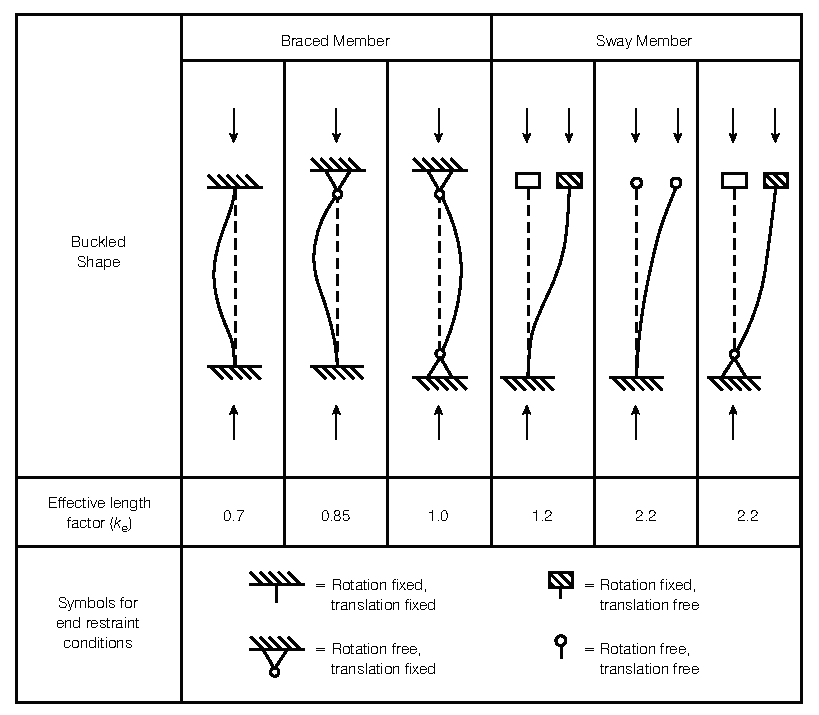
\includegraphics{PIC/CH04/BS}
\caption{Effective length factor $k_e$}\label{fig:k_e}
\end{figure}

\begin{exmp}
A \SI{10}{\meter} long 310UB32.0 beam is braced laterally (pinned) at its ends for buckling about its strong axis, and braced (pinned) at the ends and at the \textbf{quarter} points for buckling about its weak axis. Find the maximum axial compressive force it can carry.
\end{exmp}
\begin{solution}
Both strong axis and weak axis need to be considered. For a 310UB32 section, the following properties can be found: $\alpha_b=0$, $A_n=A_g=\SI{4080}{\mm^2}$, $f_y=\SI{320}{\mpa}$, $k_f=0.915$, $r_x=\SI{124}{\mm}$, $r_y=\SI{32.9}{\mm}$.
\begin{itemize}
\item strong axis ($x$-axis)\\
Since it is pinned at both ends, $k_e=1$, the modified slenderness ratio is
\begin{gather*}
\lambda_n=\dfrac{k_eL}{r_x}\sqrt{k_f}\sqrt{\dfrac{f_y}{\SI{250}{\mpa}}}=\dfrac{1\times\SI{10}{\meter}}{\SI{124}{\mm}}\times\sqrt{0.915}\times\sqrt{\dfrac{320}{250}}=87.3.
\end{gather*}
Then, $\alpha_c=0.629$. The maximum compressive force is then
\begin{gather*}
\phi{}N_{c,x}=\phi\alpha_ck_fA_nf_y=0.9\times0.629\times0.915\times\SI{4080}{\mm^2}\times\SI{320}{\mpa}=\SI{676.6}{\kn}.
\end{gather*}

This value is also given in \tabref{tab:ub_strong}.
\item weak axis ($y$-axis)\\
Since it is pinned at quarter points, $k_e=1$ and $L=0.25\times\SI{10}{\meter}=\SI{2.5}{\meter}$ the modified slenderness ratio is
\begin{gather*}
\lambda_n=\dfrac{k_eL}{r_y}\sqrt{k_f}\sqrt{\dfrac{f_y}{\SI{250}{\mpa}}}=\dfrac{1\times\SI{2.5}{\meter}}{\SI{32.9}{\mm}}\times\sqrt{0.915}\times\sqrt{\dfrac{320}{250}}=82.2.
\end{gather*}
Then, $\alpha_c=0.665$. The maximum compressive force is then
\begin{gather*}
\phi{}N_{c,y}=\phi\alpha_ck_fA_nf_y=0.9\times0.665\times0.915\times\SI{4080}{\mm^2}\times\SI{320}{\mpa}=\SI{715.0}{\kn}.
\end{gather*}

This value is also given in \tabref{tab:ub_weak}.
\end{itemize}
The governing maximum compressive force shall be the minimum of two, thus $\phi{}N_c=\SI{676.6}{\kn}$. In practice, \textbf{always} check both axes for capacity.

Note, if $L_e=\SI{0}{\m}$, then $\phi{}N_c=\phi{}N_s=0.9\times0.915\times\SI{4080}{\mm^2}\times\SI{320}{\mpa}=\SI{1075.2}{\kn}$, which are given by both tables for strong- and weak-axis buckling.
\end{solution}
\subsubsection{Frame Member}
There are two types of frame members.
\begin{itemize}
\item \textbf{Braced Frame Member}\\
In these frames, lateral stability is provided by structural walls, diagonal bracing or other similar means within the storey considered. For braced members, $1.0\geqslant{}k_e\geqslant{}0.5$.
\item \textbf{Sway Frame Member}\\
In these frames, lateral stability is provided by bending stiffness of rigidly connected beams or columns. The upper supports can also move down the same amount on each side. For sway members, $k_e\geqslant{}1.0$.
\end{itemize}

Whether the beams are braced results in different rotation constraints on beam--column joints. Besides, the illustrations in \figref{fig:fm} only show the cases when the far ends of beams are pinned. The fixity condition of beam far end also has an impact on the degree of rotation constraint offered. This will be discussed later.
\begin{figure}[ht!]
\centering
\newcommand{\BracedStructure}{
\def\a{1.5}\def\b{2}
\HingeSupport{\a,-\b}
\HingeSupport{-\a,-\b}
\RollerSupport[90]{\a,\b}
\RollerSupport[-90]{-\a,\b}
\draw[dashed](0,-\b)--++(0,2*\b);
\draw[dashed](-\a,-\b)--++(2*\a,0);
\draw[dashed](-\a,\b)--++(2*\a,0);
}
\newcommand{\SwayStructure}{
\def\a{1.5}\def\b{2}\def\c{-0.6*\a}\def\d{1.4*\a}\def\e{0.4*\a}
\HingeSupport{\a,-\b}
\HingeSupport{-\a,-\b}
\RollerSupport[90]{\d,\b}
\RollerSupport[-90]{\c,\b}
\draw[dashed](0,-\b)--++(\e,2*\b);
\draw[dashed](-\a,-\b)--++(2*\a,0);
\draw[dashed](\c,\b)--++(2*\a,0);
}
\begin{tikzpicture}[scale=1]
\begin{scope}
\BracedStructure
\draw[line width=2mm](-\a,-\b)node[joint]{}--++(2*\a,0)node[joint]{};
\draw[line width=2mm](-\a,\b)node[joint]{}--++(2*\a,0)node[joint]{};
\draw[line width=1mm](0,\b)to[out=-90,in=90](.2*\a,0)to[out=-90,in=90](0,-\b);
\node[]at(0,-\b-1){braced $k_e=0.5$};
\end{scope}
\begin{scope}[xshift=5.5cm]\def\theta{15}
\BracedStructure
\draw[line width=1mm](0,\b)to[in=90,out=-90+2*\theta](0,-\b);
\draw[line width=2mm](-\a,-\b)node[joint]{}--++(2*\a,0)node[joint]{};
\draw[line width=.3mm](-\a,\b)node[joint]{}--(0,\b)node[joint]{}--(\a,\b)node[joint]{};
\node[]at(0,-\b-1){braced $k_e=0.7$};
\end{scope}
\begin{scope}[xshift=11cm]\def\theta{15}
\BracedStructure
\draw[line width=1mm](0,\b)to[in=90-2*\theta,out=-90+2*\theta](0,-\b);
\draw[line width=.3mm](-\a,-\b)node[joint]{}--(0,-\b)node[joint]{}--(\a,-\b)node[joint]{};
\draw[line width=.3mm](-\a,\b)node[joint]{}--(0,\b)node[joint]{}--(\a,\b)node[joint]{};
\node[]at(0,-\b-1){braced $k_e=1.0$};
\end{scope}
\begin{scope}[yshift=-7cm]\def\theta{10}
\BracedStructure
\draw[line width=2mm](-\a,-\b)node[joint]{}--++(2*\a,0)node[joint]{};
\draw[line width=1mm](-\a,\b)node[joint]{}to[out=-\theta,in=180+2*\theta](0,\b)to[out=2*\theta,in=180+\theta](\a,\b)node[joint]{};
\draw[line width=1mm](0,\b)to[in=90,out=-90+2*\theta](0,-\b);
\node[]at(0,-\b-1){braced $0.5<k_e<0.7$};
\end{scope}
\begin{scope}[xshift=5.5cm,yshift=-7cm]\def\theta{10}
\BracedStructure
\draw[line width=1mm](0,\b)to[in=90-2*\theta,out=-90+2*10](0,-\b);
\draw[line width=1mm](-\a,-\b)node[joint]{}to[out=10,in=180-2*10](0,-\b)to[out=-2*10,in=180+10](\a,-\b)node[joint]{};
\draw[line width=.3mm](-\a,\b)node[joint]{}--(0,\b)node[joint]{}--(\a,\b)node[joint]{};
\node[]at(0,-\b-1){braced $0.7<k_e<1.0$};
\end{scope}
\begin{scope}[xshift=11cm,yshift=-7cm]
\SwayStructure
\draw[line width=2mm](-\a,-\b)node[joint]{}--++(2*\a,0)node[joint]{};
\draw[line width=2mm](\c,\b)node[joint]{}--++(2*\a,0)node[joint]{};
\draw[line width=1mm](\e,\b)to[in=90,out=-90](0,-\b);
\node[]at(0,-\b-1){sway $k_e=1.0$};
\end{scope}
\begin{scope}[yshift=-14cm]
\SwayStructure
\draw[line width=1mm](\e,\b)to[in=90,out=-90-10](0,-\b);
\draw[line width=2mm](-\a,-\b)node[joint]{}--++(2*\a,0)node[joint]{};
\draw[line width=.3mm](\c,\b)node[joint]{}--(\e,\b)node[joint]{}--(\d,\b)node[joint]{};
\node[]at(0,-\b-1){sway $k_e=2.0$};
\end{scope}
\begin{scope}[xshift=5.5cm,yshift=-14cm]
\SwayStructure
\draw[line width=1mm](\e,\b)--(0,-\b);
\draw[line width=.3mm](\c,\b)node[joint]{}--(\e,\b)node[joint]{}--(\d,\b)node[joint]{};
\draw[line width=.3mm](-\a,-\b)node[joint]{}--(0,-\b)node[joint]{}--(\a,-\b)node[joint]{};
\node[]at(0,-\b-1){sway $k_e=\infty$};
\end{scope}
\begin{scope}[xshift=11cm,yshift=-14cm]
\SwayStructure
\draw[line width=1mm](\c,\b)node[joint]{}to[out=20,in=180-20](\e,\b)to[out=-20,in=180+20](\d,\b)node[joint]{};
\draw[line width=1mm](-\a,-\b)node[joint]{}to[out=10,in=180-10](0,-\b)to[out=-10,in=180+10](\a,-\b)node[joint]{};
\draw[line width=1mm](\e,\b)to[in=90-10,out=-90-20](0,-\b);
\node[]at(0,-\b-1){sway $1.0<k_e<\infty$};
\end{scope}
\end{tikzpicture}
\caption{Illustration of different types of frame members with theoretical $k_e$ shown}\label{fig:fm}
\end{figure}

In order to compute member capacities, two methods are available, namely the stability function and the $\gamma$-factor method.
\paragraph{Stability Functions}
In the general case of different $EI$ in the beams at the top and bottom of the frame, stability functions can be used to evaluate the buckling force in the member without needing to consider the effective lengths. These are included in computer programs but are not studied here.
\paragraph{The $\gamma$-Factor Method}
Alternatively, for frame members, the effective length factor $k_e$ can be determined by a simplified method via stiffness ratios. The following assumptions of idealized conditions, which seldom exist in real structures, are adopted (\ANSI{\S~7.2}):
\begin{itemize}
\item all members have constant cross section,
\item all joints are rigid,
\item joint restraint is distributed to the column above and below the joint in proportion to $EI/L$ of the two columns,
\item for braced frames, rotations at opposite ends of the beams are of equal magnitude, producing single curvature bending,
\item for sway frames, rotations at opposite ends of the restraining beams are of equal magnitude, producing reverse curvature bending,
\item the stiffness parameters $L\sqrt{\dfrac{P}{EI}}$ of all columns are equal,
\item all columns buckle simultaneously,
\item behaviour is purely elastic,
\item no significant axial compression force exists in the girders,
\item shear deformations are neglected.
\end{itemize}

For each compression member, it is possible to compute the stiffness ratios of two ends respectively via the following expression.
\begin{gather}\label{eq:be}
\gamma=\dfrac{\displaystyle\sum_{\text{columns}}\dfrac{EI}{L}}{\displaystyle\sum_{\text{beams}}\dfrac{\beta_eEI}{L}}=\dfrac{\displaystyle\sum_{\text{columns}}\dfrac{I}{L}}{\displaystyle\sum_{\text{beams}}\dfrac{\beta_eI}{L}},
\end{gather}
in which
\begin{itemize}
\item \NZSSTEEL{\S~4.8.3.4.2} $\displaystyle\sum_{\text{columns}}\dfrac{I}{L}$ shall be calculated from the sum of the stiffnesses, in the plane of bending, of all the compression members rigidly connected at the end of the member under consideration, including the member itself.
\item \NZSSTEEL{\S~4.8.3.4.3} $\displaystyle\sum_{\text{beams}}\dfrac{\beta_eI}{L}$ shall be calculated from the sum of the stiffnesses, in the plane of bending, of all the beams rigidly connected at the end of the member under consideration. The contributions of any beams pin-connected to the member shall be neglected.
\item $\beta_e$ is a modification factor to account for different beam far end conditions. This will be introduced later. For the moment, assume $\beta_e=1$.
\end{itemize}

With $\gamma_1$ and $\gamma_2$ (for two ends) at hand, $k_e$ can be calculated by one of the following methods:
\begin{enumerate}
\item The exact solution for the assumptions above may be found using the following equations. These are transcendental functions that can be solved by numerical methods.
\begin{itemize}
\item braced member
\begin{gather*}
\dfrac{\gamma_1\gamma_2}{4}\left(\dfrac{\pi}{k_e}\right)^2+\dfrac{\gamma_1+\gamma_2}{2}\left(1-\dfrac{\pi/k_e}{\tan\left(\pi/k_e\right)}\right)+\dfrac{2\tan\left(0.5\pi/k_e\right)}{\pi/k_e}=1.0
\end{gather*}
\item sway member
\begin{gather*}
\left(\gamma_1\gamma_2\left(\dfrac{\pi}{k_e}\right)^2-36\right)\tan\left(\dfrac{\pi}{k_e}\right)=6\left(\gamma_1+\gamma_2\right)\dfrac{\pi}{k_e}
\end{gather*}
\end{itemize}
\item US Alignment Charts. These charts used in \ANSI{} give the graphical solutions to the two equations above. They are shown in \figref{fig:a360_ke} in which $G_A$ and $G_B$ correspond to $\gamma_1$ and $\gamma_2$. Additional copies are provided at the end of this chapter.
\begin{figure}[htb!]
\centering\footnotesize
\begin{subfigure}{.5\linewidth}\centering
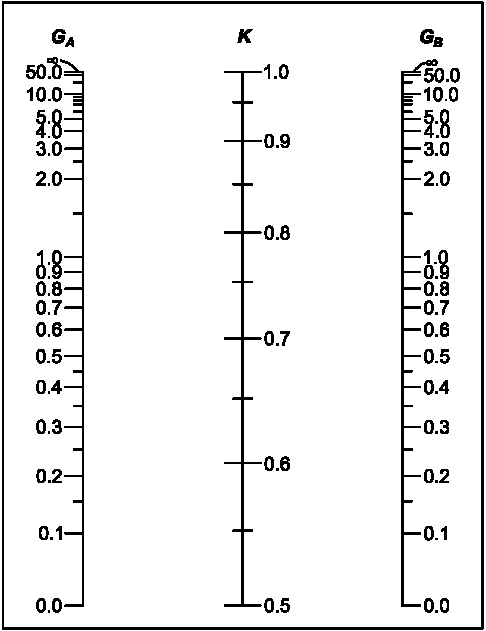
\includegraphics[width=.9\linewidth]{PIC/CH04/A360.BRACED}
\caption{for braced members}
\end{subfigure}\hfil
\begin{subfigure}{.5\linewidth}\centering
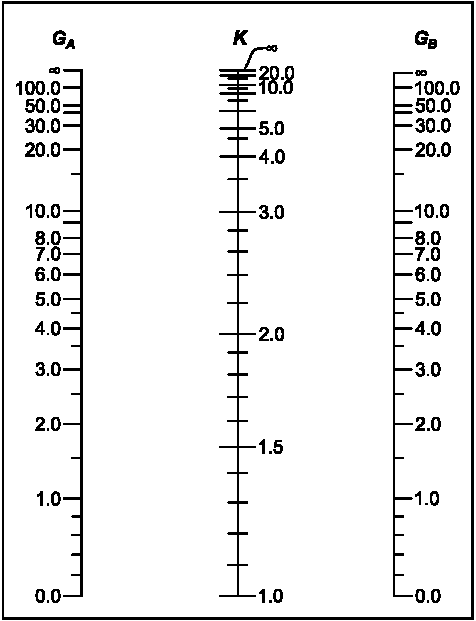
\includegraphics[width=.9\linewidth]{PIC/CH04/A360.SWAY}
\caption{for sway members}
\end{subfigure}
\caption{Alignment chart for $k_e$}\label{fig:a360_ke}
\end{figure}
\item AU/NZ Alignment Charts. These charts used in \NZSSTEEL{Fig. 4.8.3.3} are essentially identical to the ones used in the US code but presented in a different format. \figref{fig:kee} shows those charts.
\begin{figure}[H]
\centering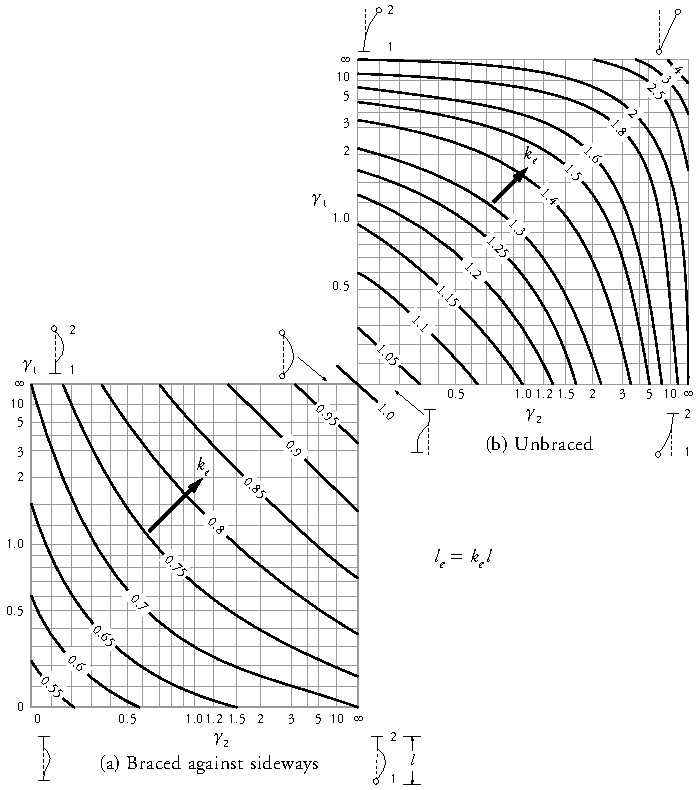
\includegraphics[width=.99\textwidth]{PIC/CH04/KEE}
\caption{$k_e$ for braced and sway members \citep{Gorenc2015}}\label{fig:kee}
\end{figure}
\item French Equations. These are used in the French code and they are an approximation to the two equations above. They give answers to an accuracy of better than \SI{1}{\percent} to the true answer and any error results in a slightly conservative answer. This is better than the readability of the design charts.
\begin{itemize}
\item braced member
\begin{gather}\color{cc0066}
k_e=\dfrac{3\gamma_1\gamma_2+1.4\left(\gamma_1+\gamma_2\right)+0.64}{3\gamma_1\gamma_2+2\left(\gamma_1+\gamma_2\right)+1.28}
\end{gather}
\item sway member
\begin{gather}\color{cc0066}
k_e=\sqrt{\dfrac{1.6\gamma_1\gamma_2+4\left(\gamma_1+\gamma_2\right)+7.5}{\gamma_1+\gamma_2+7.5}}
\end{gather}
\end{itemize}
\end{enumerate}
The French method is probably the best for practical usage, although any of the methods above would be acceptable.
\subsubsection{Examples of Alignment Charts}
To use the alignment charts, one shall calculate $\gamma_1$ and $\gamma_2$ first. Draw a straight line defined by $\gamma_1$ and $\gamma_2$, the intersection gives the value of $k_e$.
\paragraph{Braced Individual Member}
Since both ends are fixed,
\begin{gather*}
\gamma_{top}=\gamma_{bot}=0.
\end{gather*}
From the chart, $k_e=0.5$.
\begin{figure}[H]
\centering
\footnotesize
\begin{tikzpicture}
\draw[draw=none](-1,-1)rectangle(4,4);
\FixedSupport{0,0}
\SleeveSupport{0,3}
\draw[line width=1.2mm,cc0066](0,0)--(0,3);
\node[anchor=south]at(-6,-1){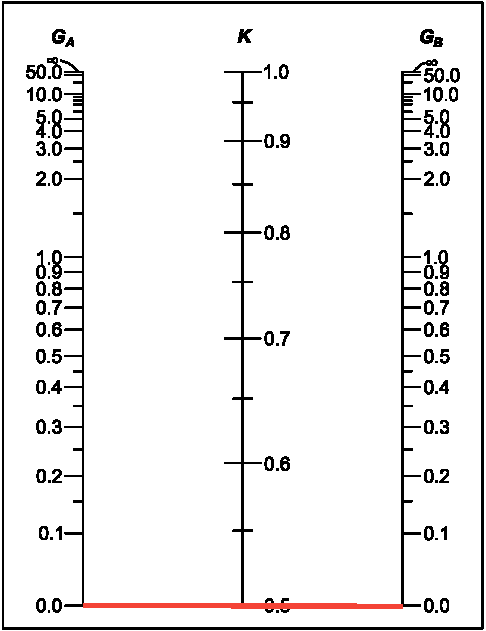
\includegraphics[width=5cm]{PIC/CH04/A360.BRACEDEX1}};
\end{tikzpicture}
\end{figure}
\paragraph{Braced Frame Member}
The top end is connected to two beams,
\begin{gather*}
\gamma_{top}=\dfrac{1}{1.5/0.8+1.5/1.5}=0.348,\qquad
\gamma_{bot}=0.
\end{gather*}
From the chart, $k_e\approx0.57$. The French equation gives $k_e=0.5704$.
\begin{figure}[H]
\centering
\footnotesize
\begin{tikzpicture}
\draw[draw=none](-1,-1)rectangle(4,4);
\FixedSupport{0,0}
\FixedSupport{3,0}
\FixedSupport{2,0}
\RollerSupport[90]{3,3}
\draw[line width=1.2mm,draw=black!20](0,0)|-(3,3)--(3,0);
\draw[line width=1.2mm,cc0066](2,3)--(2,0);
\node[above]at(1,3){$1.5L$};
\node[above]at(2.5,3){$0.8L$};
\node[below]at(1,3){$1.5I$};
\node[below]at(2.5,3){$1.5I$};
\node[right]at(2,1.5){$I$};
\node[left]at(2,1.5){$L$};
\node[anchor=south]at(-6,-1){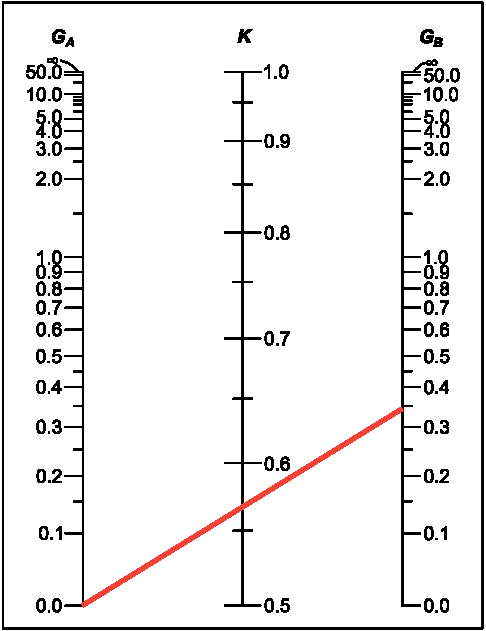
\includegraphics[width=5cm]{PIC/CH04/A360.BRACEDEX2}};
\end{tikzpicture}
\end{figure}
\paragraph{Sway Individual Member}
Since the top end is a free end and the bottom end is fixed,
\begin{gather*}
\gamma_{top}=\infty,\qquad\gamma_{bot}=0.
\end{gather*}
From the chart, $k_e=2.0$.
\begin{figure}[H]
\centering
\footnotesize
\begin{tikzpicture}
\draw[draw=none](-1,-1)rectangle(4,4);
\FixedSupport{0,0}
\draw[line width=1.2mm,cc0066](0,0)--(0,3);
\node[anchor=south]at(-6,-1){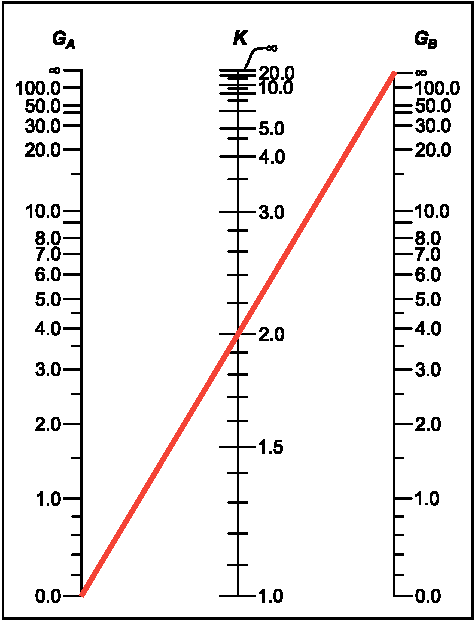
\includegraphics[width=5cm]{PIC/CH04/A360.SWAYEX1}};
\end{tikzpicture}
\end{figure}
\paragraph{Sway Frame Member}
The top end is connected to two beams,
\begin{gather*}
\gamma_{top}=\dfrac{1}{1.5/0.8+1.5/1.5}=0.348,\qquad
\gamma_{bot}=0.
\end{gather*}
From the chart, $k_e\approx1.05$. The French equation gives $k_e=1.0644$.
\begin{figure}[H]
\centering
\footnotesize
\begin{tikzpicture}
\draw[draw=none](-1,-1)rectangle(4,4);
\FixedSupport{0,0}
\FixedSupport{3,0}
\FixedSupport{2,0}
\draw[line width=1.2mm,draw=black!20](0,0)|-(3,3)--(3,0);
\draw[line width=1.2mm,cc0066](2,3)--(2,0);
\node[above]at(1,3){$1.5L$};
\node[above]at(2.5,3){$0.8L$};
\node[below]at(1,3){$1.5I$};
\node[below]at(2.5,3){$1.5I$};
\node[right]at(2,1.5){$I$};
\node[left]at(2,1.5){$L$};
\node[anchor=south]at(-6,-1){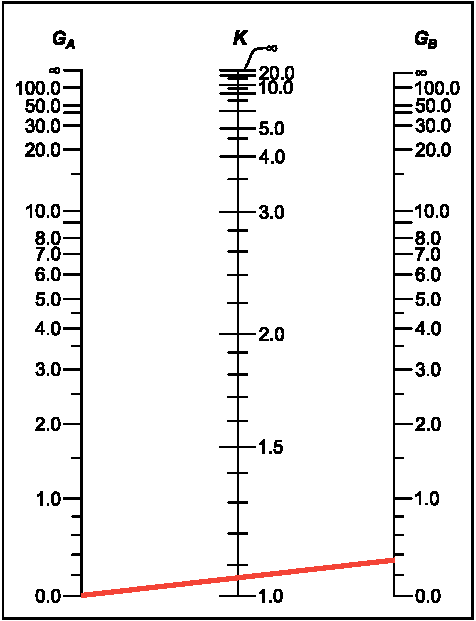
\includegraphics[width=5cm]{PIC/CH04/A360.SWAYEX2}};
\end{tikzpicture}
\end{figure}
\subsubsection{Remark}
The stiffness ratio $\gamma$ characterises the rotation ability of an end. A sufficiently large $\gamma\rightarrow\infty$ represents a pinned connection while a sufficiently small $\gamma\rightarrow0$ represents a fixed connection. \textbf{However, those are idealised assumptions, in real world those perfect connections do not exist. Thus, $\gamma$ is often taken as \num{1} for fully fixed connection and \num{10} for perfectly pinned connection.}

\begin{exmp}\href{run:./WORKSHEET/CH04/EX4.ACFM.sm}{Worksheet}
Axial Compression Example --- Frame

For the frame shown, find axial compression capacity of column when the frame is a) braced and b) unbraced. Assume the out-of-plane buckling is fully prevented and in-plane deformations cause strong axis member bending. Use Grade 300 steel.
\begin{figure}[H]
\footnotesize
\begin{tikzpicture}[scale=.6]
\HingeSupport{0,0}{1.5}
\HingeSupport{7,0}{1.5}
\draw[line width=1mm](0,0)node[draw,circle,line width=.6mm,inner sep=0,minimum size=2.5mm,fill=exmpbg]{}--++(0,5)--++(7,0)--++(0,-5)node[draw,circle,line width=.6mm,inner sep=0,minimum size=2.5mm,fill=exmpbg]{};
\draw[|<->|](0,-1)--++(7,0)node[midway,fill=exmpbg]{\SI{7}{\meter}};
\draw[|<->|](-1,0)--++(0,5)node[midway,fill=exmpbg]{\SI{5}{\meter}};
\setstructmech{convention=direction}
\NodalForce{0,7}[N][-P][N]
\NodalForce{7,7}[N][-P][N]
\node[align=left]at(3.5,2.5){Beam: 360UB56.7\\Column: 530UB82.0};
\end{tikzpicture}
\end{figure}
\end{exmp}
\begin{solution}
In this simple case, $\beta_e=1$. The stiffness ratios can be computed as
\begin{gather*}
\gamma_1=\gamma_{top}=\dfrac{I_c/L_c}{\beta_eI_b/L_b}=4.15,\qquad
\gamma_2=\gamma_{bot}=10.
\end{gather*}
Note for the pinned connection, \num{10} is used.
\begin{itemize}
\item braced frame

By the French equation,
\begin{gather*}
k_e=\dfrac{3\gamma_1\gamma_2+1.4\left(\gamma_1+\gamma_2\right)+0.64}{3\gamma_1\gamma_2+2\left(\gamma_1+\gamma_2\right)+1.28}=0.941.
\end{gather*}
The modified slenderness ratio,
\begin{gather*}
\lambda_n=\dfrac{k_eL}{r_x}\sqrt{k_f}\sqrt{\dfrac{f_y}{\SI{250}{\mpa}}}=\dfrac{0.941\times\SI{5}{\meter}}{\SI{213}{\mm}}\times\sqrt{0.902}\times\sqrt{\dfrac{300}{250}}=22.97.
\end{gather*}
Thus $\alpha_c=0.968$,
\begin{gather*}
\phi{}N_c=\phi\alpha_ck_fA_nf_y=0.9\times0.968\times0.902\times\SI{10500}{\mm^2}\times\SI{300}{\mpa}=\SI{2475}{\kn}.
\end{gather*}
\item sway frame

By the French equation,
\begin{gather*}
k_e=\sqrt{\dfrac{1.6\gamma_1\gamma_2+4\left(\gamma_1+\gamma_2\right)+7.5}{\gamma_1+\gamma_2+7.5}}=2.455.
\end{gather*}
The modified slenderness ratio,
\begin{gather*}
\lambda_n=\dfrac{k_eL}{r_x}\sqrt{k_f}\sqrt{\dfrac{f_y}{\SI{250}{\mpa}}}=\dfrac{2.455\times\SI{5}{\meter}}{\SI{213}{\mm}}\times\sqrt{0.902}\times\sqrt{\dfrac{300}{250}}=59.95.
\end{gather*}
Thus $\alpha_c=0.809$,
\begin{gather*}
\phi{}N_c=\phi\alpha_ck_fA_nf_y=0.9\times0.809\times0.902\times\SI{10500}{\mm^2}\times\SI{300}{\mpa}=\SI{2069}{\kn}.
\end{gather*}
\end{itemize}
\end{solution}

%
%\begin{exmp}
%Axial Compression Example --- Braced Frame
%
%For the following frame supported out-of-plane at top and bottom only, find the lightest Grade 300 I section to carry the load $N^*=\SI{700}{\kn}$.
%\end{exmp}
%\begin{solution}
%Noting that $L_{e,x}=4\times\SI{4.5}{\meter}=\SI{18}{\meter}$ while $L_{e,y}=\SI{4.5}{\meter}$, an efficient member shall have similar slenderness ratios $\lambda=L_e/r$ about both axes.
%
%Thus we try UB sections only.
%\end{solution}
\subsection{Modifications to \texorpdfstring{$\gamma$}{G}-Factor Method}
\subsubsection{Effect of Beam End Conditions}
Recall \figref{fig:fm} and \eqsref{eq:be},
\begin{gather*}
\gamma=\dfrac{\displaystyle\sum_{\text{columns}}\dfrac{EI}{L}}{\displaystyle\sum_{\text{beams}}\dfrac{\beta_eEI}{L}}=\dfrac{\displaystyle\sum_{\text{columns}}\dfrac{I}{L}}{\displaystyle\sum_{\text{beams}}\dfrac{\beta_eI}{L}}.
\end{gather*}

\NZSSTEEL{\S~4.8.3.4.3} uses a modifying factor $\beta_e$ to account for various conditions at the far ends of the beams, which may affect the magnitude of moment on the joint. This corresponds to \ANSI{Eq. C-A-7-4}.
\begin{table}[H]
\centering\footnotesize
\caption{Modifying factor $\beta_e$}\label{tab:beta_e}
\begin{tabular}{lrr}
	\toprule
	fixity at far end of beam     & beam restraining a braced member & beam restraining a sway member \\ \midrule
	pinned                        &                              1.5 &                            0.5 \\
	rigidly connected to a column &                              1.0 &                            1.0 \\
	fixed                         &                              2.0 &                           0.67 \\ \bottomrule
\end{tabular}
\end{table}
\begin{figure}[H]
\centering
\footnotesize
\newcommand{\BaseStruct}{
\draw[line width=1.2mm](0,0)|-(3,3);
\node[draw,inner sep=0,minimum size=2.5mm,circle,fill=white,line width=.6mm]at(0,0){};
\node[draw,inner sep=0,minimum size=2.5mm,circle,fill=white,line width=.6mm]at(3,3){};
}
\newcommand{\BaseStructX}{
\draw[line width=1.2mm](0,0)|-(3,3);
\node[draw,inner sep=0,minimum size=2.5mm,circle,fill=white,line width=.6mm]at(0,0){};
}
\newcommand{\BaseStructS}{
\draw[line width=1.2mm](0,0)|-(3,3)--(3,0);
\node[draw,inner sep=0,minimum size=2.5mm,circle,fill=white,line width=.6mm]at(0,0){};
\node[draw,inner sep=0,minimum size=2.5mm,circle,fill=white,line width=.6mm]at(3,0){};
}
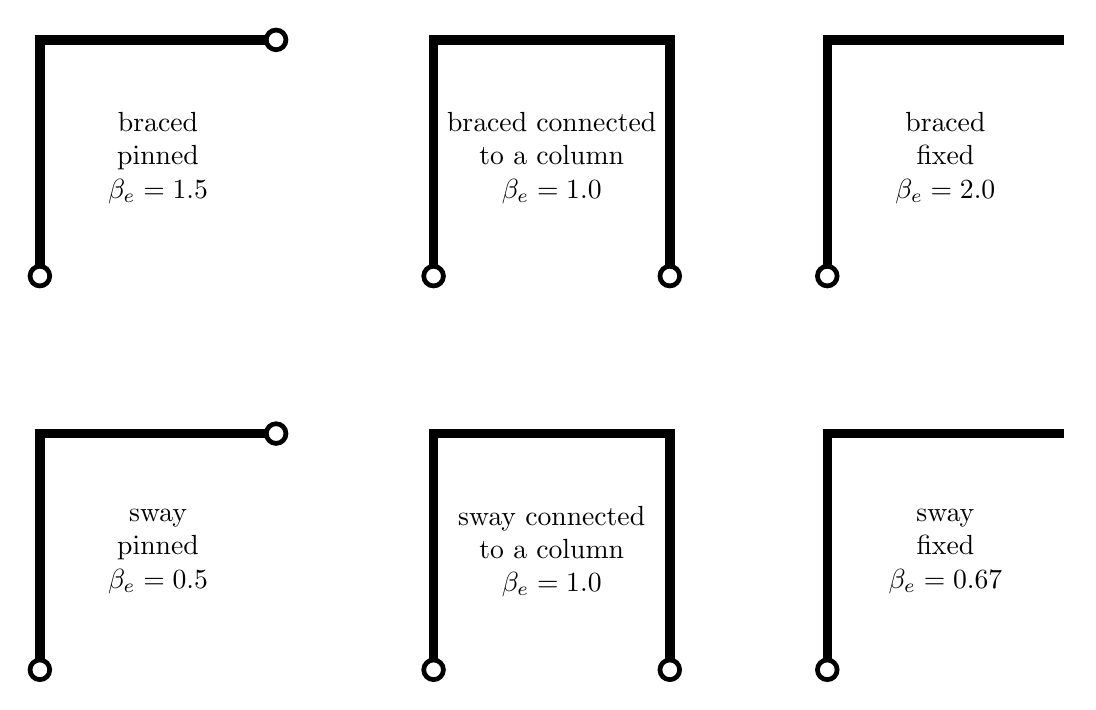
\begin{tikzpicture}
\begin{scope}
\HingeSupport{0,0}
\HingeSupport[90]{3,3}
\BaseStruct
\node[align=center]at(1.5,1.5){braced\\pinned\\$\beta_e=1.5$};
\end{scope}
\begin{scope}[xshift=5cm]
\HingeSupport{0,0}
\HingeSupport{3,0}
\RollerSupport[90]{3,3}
\BaseStructS
\node[align=center]at(1.5,1.5){braced connected\\to a column\\$\beta_e=1.0$};
\end{scope}
\begin{scope}[xshift=10cm]
\HingeSupport{0,0}
\FixedSupport[90]{3,3}
\BaseStructX
\node[align=center]at(1.5,1.5){braced\\fixed\\$\beta_e=2.0$};
\end{scope}
\begin{scope}[yshift=-5cm]
\HingeSupport{0,0}
\RollerSupport{3,3}
\BaseStruct
\node[align=center]at(1.5,1.5){sway\\pinned\\$\beta_e=0.5$};
\end{scope}
\begin{scope}[xshift=5cm,yshift=-5cm]
\HingeSupport{0,0}
\HingeSupport{3,0}
\BaseStructS
\node[align=center]at(1.5,1.5){sway connected\\to a column\\$\beta_e=1.0$};
\end{scope}
\begin{scope}[xshift=10cm,yshift=-5cm]
\HingeSupport{0,0}
\SleeveSupport[90]{3,3}
\BaseStructX
\node[align=center]at(1.5,1.5){sway\\fixed\\$\beta_e=0.67$};
\end{scope}
\end{tikzpicture}
\caption{Far end of beam conditions}
\end{figure}
\subsubsection{Member Yielding}
Stocky columns which are subject to high axial forces may yield as a result of the residual stress. This reduces the elastic modulus, so the column has a `close to' pinned connection at the yield end. This can lead to a saving of material.

We will not study this in this class, and it is not important for $f<0.5f_y$.
\subsubsection{Total Storey Sidesway}
The design charts are based on the assumption that all columns buckle simultaneously and that the sidesway load for the storey can be obtained from the sidesway load of one column.

In gravity frames the resistance of one column to sidesway may be greater than that of other columns due to its loading or stiffness. It is assumed columns are axially rigid.

For design against sidesway, the gravity load which a frame can support may be split up in any proportion. An example is shown as follows.
\begin{figure}[H]
\centering\footnotesize
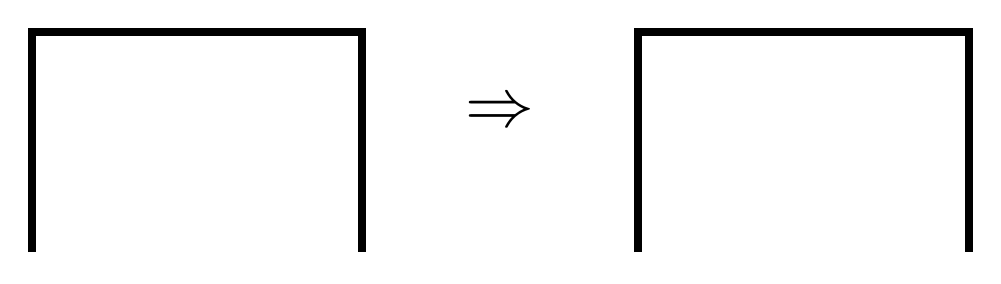
\begin{tikzpicture}[scale=.7]
\begin{scope}
\FixedSupport{0,0}
\FixedSupport{6,0}
\draw[line width=1mm](0,0)--++(0,4)--++(6,0)--++(0,-4);
\setstructmech{convention=direction}
\NodalForce{0,6}[N][-\SI{200}{\kn}][N]
\NodalForce{6,6}[N][-\SI{400}{\kn}][N]
\end{scope}
\begin{scope}[xshift=11cm]
\FixedSupport{0,0}
\FixedSupport{6,0}
\draw[line width=1mm](0,0)--++(0,4)--++(6,0)--++(0,-4);
\setstructmech{convention=direction}
\NodalForce{0,6}[N][-\SI{600}{\kn}][N]
\NodalForce{6,6}[N][-\SI{0}{\kn}][N]
\end{scope}
\node at(8.5,2.5){\Huge$\Rightarrow$};
\end{tikzpicture}
\caption{Transfer of vertical loads}
\end{figure}

However, the maximum load in any column must \textbf{not} exceed the maximum load that a column could support if it were braced against sidesway ($k_e=1.0$).

For the following frame, assume the braced and sway capacities for each column are listed as follows.
\begin{figure}[H]
\centering\footnotesize
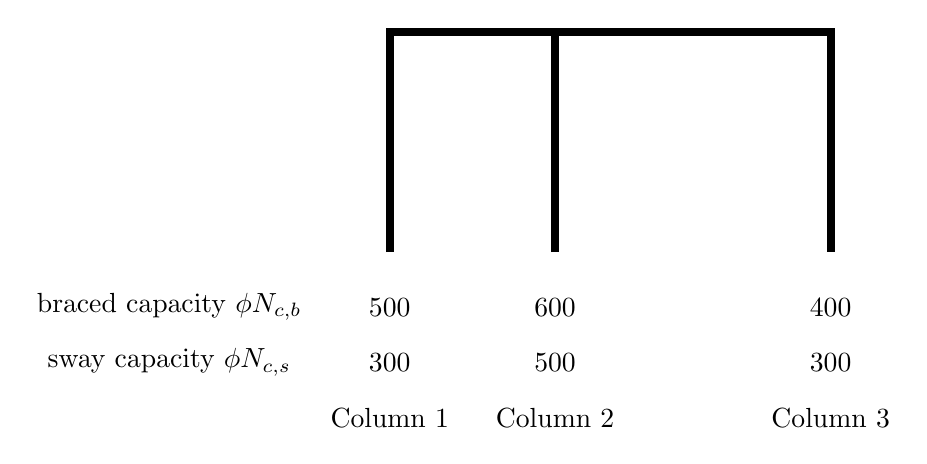
\begin{tikzpicture}[scale=.7]
\begin{scope}
\FixedSupport{0,0}
\FixedSupport{3,0}
\FixedSupport{8,0}
\draw[line width=1mm](0,0)--++(0,4)--++(8,0)--++(0,-4)(3,0)--++(0,4);
\setstructmech{convention=direction}
\node at(-4,-1){braced capacity $\phi{}N_{c,b}$};
\node at(0,-1){\SI{500}{\kn}};
\node at(3,-1){\SI{600}{\kn}};
\node at(8,-1){\SI{400}{\kn}};
\node at(-4,-2){sway capacity $\phi{}N_{c,s}$};
\node at(0,-2){\SI{300}{\kn}};
\node at(3,-2){\SI{500}{\kn}};
\node at(8,-2){\SI{300}{\kn}};
\node at(0,-3){Column 1};
\node at(3,-3){Column 2};
\node at(8,-3){Column 3};
\end{scope}
\end{tikzpicture}
\end{figure}
For the sway mechanism, $\sum_{i=1}^3N^*_i=N^*\leqslant\sum_{i=1}^3\phi{}N_{c,s}^i=\SI{1100}{\kn}$. For each column, the maximum load shall not exceed its braced capacity, that is
\begin{gather*}
N^*_1\leqslant\phi{}N_{c,b}^1=\SI{500}{\kn},\qquad
N^*_2\leqslant\phi{}N_{c,b}^2=\SI{600}{\kn},\qquad
N^*_3\leqslant\phi{}N_{c,b}^3=\SI{400}{\kn}.
\end{gather*}

Now consider the following two cases.
\begin{itemize}
\item The loads for columns 1 and 2 are given as $N^*_1=\SI{400}{\kn}$ and $N^*_2=\SI{500}{\kn}$, what is the maximum load of column 3?\\Knowing that $N^*\leqslant\SI{1100}{\kn}$ to prevent sway mechanism, $N^*_3\leqslant\SI{1100}{\kn}-\SI{400}{\kn}-\SI{500}{\kn}=\SI{200}{\kn}$. Thus the maximum load of column 3 should be $N^*_3=\min\left(\SI{200}{\kn},~\SI{400}{\kn}\right)=\SI{200}{\kn}$.
\item The loads for columns 1 and 2 are given as $N^*_1=\SI{300}{\kn}$ and $N^*_2=\SI{300}{\kn}$, what is the maximum load of column 3?\\Knowing that $N^*\leqslant\SI{1100}{\kn}$ to prevent sway mechanism, $N^*_3\leqslant\SI{1100}{\kn}-\SI{300}{\kn}-\SI{300}{\kn}=\SI{500}{\kn}$. Thus the maximum load of column 3 should be $N^*_3=\min\left(\SI{500}{\kn},~\SI{400}{\kn}\right)=\SI{400}{\kn}$.
\end{itemize}
\subsubsection{Use of Effective Length Factor --- Practical Considerations}
For columns in braced frames, it is always conservative to use $k_e=1$. This has been recommended by \citet{Yura1971}. Based on this, and the uncertainty in assessing some of these connection stiffness, we will use $k_e=1$ for the braced case consideration for columns in
\begin{enumerate}
\item sway frames, and
\item braced frames, where there is loading along the beam length causing column moment.
\end{enumerate}
For columns in braced frames with no moment from the beams, $k_e$ can be computed as being less than \num{1} using the techniques described above.

\begin{exmp}\href{run:./WORKSHEET/CH04/EX4.ACSF.sm}{Worksheet}
Axial Compression Example --- Sway Frame

For the frame shown, the columns are supported out-of-plane at top, centre and bottom, find 1) the maximum value of axial load each column can carry and 2) the maximum value of $N^*_1+N^*_2$ the frame can carry. Note the out-of-plane (weak axis) buckling should be checked as well. Use Grade 300 steel.
\begin{figure}[H]
\footnotesize
\begin{tikzpicture}[scale=.6]
\FixedSupport{0,0}{1.5}
\FixedSupport{7,0}{1.5}
\draw[line width=1mm](0,0)--++(0,5)--++(7,0)--++(0,-5);
\draw[|<->|](0,-1)--++(7,0)node[midway,fill=exmpbg]{\SI{7}{\meter}};
\draw[|<->|](-1,0)--++(0,5)node[midway,fill=exmpbg]{\SI{5}{\meter}};
\setstructmech{convention=direction}
\NodalForce{0,7}[N][-N^*_1][N]
\NodalForce{7,7}[N][-N^*_2][N]
\RollerSupport[120]{0,2.5}{1.5}
\RollerSupport[120]{7,2.5}{1.5}
\draw[dashed](0,2.5)--++(30:2);
\draw[dashed](7,2.5)--++(30:2);
\node[align=left]at(4,2){Beam: 410UB53.7\\Left Column: 250UC89.5\\Right Column: 250UC72.9};
\node at(15,2.5){
\begin{tabular}{cccccc}
	\toprule
	          &     $A$     &                   $I_x$                    &   $r_x$   &   $r_y$    &   $f_y$   \\
	          & \si{\mm^2}  & \SI[print-unity-mantissa=false]{e6}{\mm^6} & \si{\mm}  &  \si{\mm}  & \si{\mpa} \\ \midrule
	410UB53.7 &             &                 \num{188}                  &           &            &           \\
	250UC89.5 & \num{11400} &                 \num{143}                  & \num{112} & \num{65.2} & \num{280} \\
	250UC72.9 & \num{9320}  &                 \num{114}                  & \num{111} & \num{64.5} & \num{300} \\ \bottomrule
\end{tabular}
};
\end{tikzpicture}
\end{figure}
\end{exmp}
\begin{solution}
\begin{itemize}
\item For sway capacity.

\begin{itemize}
\item Left Column\\
Find stiffness ratios. $\gamma_{bot}=\gamma_2=1$.
\begin{gather*}
\gamma_{top}=\gamma_1=\dfrac{I_c/L_c}{\beta_eI_b/L_b}=\dfrac{\SI{143e6}{\mm^6}/\SI{5}{\meter}}{1\times\SI{188e6}{\mm^6}/\SI{7}{\meter}}=1.065.
\end{gather*}
From French equation, $k_e=1.351$. Thus, the modified slenderness ratio,
\begin{gather*}
\lambda_n=\dfrac{k_eL_x}{r_x}\sqrt{k_f}\sqrt{\dfrac{f_y}{\SI{250}{\mpa}}}=\dfrac{1.351\times\SI{5}{\meter}}{\SI{112}{\mm}}\times\sqrt{1}\times\sqrt{\dfrac{280}{250}}=63.84.
\end{gather*}
Thus $\alpha_c=0.786$,
\begin{gather*}
\phi{}N_c=\phi\alpha_ck_fA_nf_y=0.9\times0.786\times1\times\SI{11400}{\mm^2}\times\SI{280}{\mpa}=\SI{2259}{\kn}.
\end{gather*}

Alternatively, $L_e=k_eL_x=\SI{6.76}{\m}$ could be used to get \SI{2259}{\kn} by linear interpolation from \tabref{tab:uc_strong}.
\item Right Column\\
Find stiffness ratios. $\gamma_{bot}=\gamma_2=1$.
\begin{gather*}
\gamma_{top}=\gamma_1=\dfrac{I_c/L_c}{\beta_eI_b/L_b}=\dfrac{\SI{114e6}{\mm^6}/\SI{5}{\meter}}{1\times\SI{188e6}{\mm^6}/\SI{7}{\meter}}=0.849.
\end{gather*}
From French equation, $k_e=1.319$. Thus, the modified slenderness ratio,
\begin{gather*}
\lambda_n=\dfrac{k_eL_x}{r_x}\sqrt{k_f}\sqrt{\dfrac{f_y}{\SI{250}{\mpa}}}=\dfrac{1.319\times\SI{5}{\meter}}{\SI{111}{\mm}}\times\sqrt{1}\times\sqrt{\dfrac{300}{250}}=65.06.
\end{gather*}
Thus $\alpha_c=0.779$,
\begin{gather*}
\phi{}N_c=\phi\alpha_ck_fA_nf_y=0.9\times0.779\times1\times\SI{9320}{\mm^2}\times\SI{300}{\mpa}=\SI{1961}{\kn}.
\end{gather*}

Alternatively, $L_e=k_eL_x=\SI{6.60}{\m}$ could be used to get \SI{1961}{\kn} by linear interpolation from \tabref{tab:uc_strong}.
\end{itemize}
Thus the total $N^*=\sum{}N^*_i=\SI{2259}{\kn}+\SI{1961}{\kn}=\SI{4220}{\kn}$.
\item For braced capacity.

One can use French equation to find the corresponding $k_e$ as shown before. For braced columns in a sway frame, use $k_e=1$.
\begin{itemize}
\item Left Column\\
The modified slenderness ratio,
\begin{gather*}
\lambda_n=\dfrac{k_eL_x}{r_x}\sqrt{k_f}\sqrt{\dfrac{f_y}{\SI{250}{\mpa}}}=\dfrac{1\times\SI{5}{\meter}}{\SI{112}{\mm}}\times\sqrt{1}\times\sqrt{\dfrac{280}{250}}=47.25.
\end{gather*}
Thus, $\alpha_c=0.874$.
\begin{gather*}
\phi{}N_c=\phi\alpha_ck_fA_nf_y=0.9\times0.874\times1\times\SI{11400}{\mm^2}\times\SI{280}{\mpa}=\SI{2509}{\kn}.
\end{gather*}
\item Right Column\\
The modified slenderness ratio,
\begin{gather*}
\lambda_n=\dfrac{k_eL_x}{r_x}\sqrt{k_f}\sqrt{\dfrac{f_y}{\SI{250}{\mpa}}}=\dfrac{1\times\SI{5}{\meter}}{\SI{111}{\mm}}\times\sqrt{1}\times\sqrt{\dfrac{300}{250}}=49.34.
\end{gather*}
Thus, $\alpha_c=0.864$.
\begin{gather*}
\phi{}N_c=\phi\alpha_ck_fA_nf_y=0.9\times0.864\times1\times\SI{9320}{\mm^2}\times\SI{300}{\mpa}=\SI{2173}{\kn}.
\end{gather*}
\end{itemize}
From $\alpha_c$, one can tell the braced capacity shall be greater than the sway capacity.
\item For weak axis buckling.

Again, we choose $k_e=1$ for a conservative design. Since the columns are supported every half the length, $L_y=\SI{2.5}{\meter}$.
\begin{itemize}
\item Left Column\\
The modified slenderness ratio,
\begin{gather*}
\lambda_n=\dfrac{k_eL_y}{r_y}\sqrt{k_f}\sqrt{\dfrac{f_y}{\SI{250}{\mpa}}}=\dfrac{1\times\SI{2.5}{\meter}}{\SI{65.2}{\mm}}\times\sqrt{1}\times\sqrt{\dfrac{280}{250}}=40.58.
\end{gather*}
Thus, $\alpha_c=0.902$.
\begin{gather*}
\phi{}N_c=\phi\alpha_ck_fA_nf_y=0.9\times0.902\times1\times\SI{11400}{\mm^2}\times\SI{280}{\mpa}=\SI{2592}{\kn}.
\end{gather*}
\item Right Column\\
The modified slenderness ratio,
\begin{gather*}
\lambda_n=\dfrac{k_eL_y}{r_y}\sqrt{k_f}\sqrt{\dfrac{f_y}{\SI{250}{\mpa}}}=\dfrac{1\times\SI{2.5}{\meter}}{\SI{64.5}{\mm}}\times\sqrt{1}\times\sqrt{\dfrac{300}{250}}=42.46.
\end{gather*}
Thus, $\alpha_c=0.895$.
\begin{gather*}
\phi{}N_c=\phi\alpha_ck_fA_nf_y=0.9\times0.895\times1\times\SI{9320}{\mm^2}\times\SI{300}{\mpa}=\SI{2251}{\kn}.
\end{gather*}
\end{itemize}
The results match the capacity table well.
\end{itemize}
To sum up, the following design criteria shall be met.
\begin{gather*}
N^*_1\leqslant\min\left(\SI{2509}{\kn},~\SI{2592}{\kn}\right)=\SI{2509}{\kn},\\
N^*_2\leqslant\min\left(\SI{2173}{\kn},~\SI{2251}{\kn}\right)=\SI{2173}{\kn},\\
N^*_1+N^*_2\leqslant\SI{4220}{\kn}.
\end{gather*}

If $N^*_1=\SI{2500}{\kn}$, the frame fails with a sway mode when
\begin{gather*}
N^*_2=\min\left(\SI{2173}{\kn},\SI{4220}{\kn}-N^*_1\right)=\SI{1720}{\kn}.
\end{gather*}
\end{solution}

\begin{exmp}\href{run:./WORKSHEET/CH04/EX4.ACSF.sm}{Worksheet}
Axial Compression Example --- Braced Frame

Same as the previous example but the frame is now braced.
\begin{figure}[H]
\footnotesize
\begin{tikzpicture}[scale=.6]
\HingeSupport[90]{7,5}{1.5}
\FixedSupport{0,0}{1.5}
\FixedSupport{7,0}{1.5}
\draw[line width=1mm](0,0)--++(0,5)--++(7,0)--++(0,-5);
\draw[|<->|](0,-1)--++(7,0)node[midway,fill=exmpbg]{\SI{7}{\meter}};
\draw[|<->|](-1,0)--++(0,5)node[midway,fill=exmpbg]{\SI{5}{\meter}};
\setstructmech{convention=direction}
\NodalForce{0,7}[N][-N^*_1][N]
\NodalForce{7,7}[N][-N^*_2][N]
\RollerSupport[120]{0,2.5}{1.5}
\RollerSupport[120]{7,2.5}{1.5}
\draw[dashed](0,2.5)--++(30:2);
\draw[dashed](7,2.5)--++(30:2);
\node[align=left]at(4,2){Beam: 410UB53.7\\Left Column: 250UC89.5\\Right Column: 250UC72.9};
\end{tikzpicture}
\end{figure}
\end{exmp}
\begin{solution}
Since now the frame is braced, we use French equation to obtain $k_e$ for strong axis buckling.
\begin{itemize}
\item Column 1.

Given that $\gamma_1=1.065$ and $\gamma_2=1$, from French equation,
\begin{gather*}
k_e=\dfrac{3\gamma_1\gamma_2+1.4\left(\gamma_1+\gamma_2\right)+0.64}{3\gamma_1\gamma_2+2\left(\gamma_1+\gamma_2\right)+1.28}=0.782.
\end{gather*}
Then,
\begin{gather*}
\lambda_n=\dfrac{k_eL_x}{r_x}\sqrt{k_f}\sqrt{\dfrac{f_y}{\SI{250}{\mpa}}}=\dfrac{0.782\times\SI{5}{\meter}}{\SI{112}{\mm}}\times\sqrt{1}\times\sqrt{\dfrac{280}{250}}=36.93.
\end{gather*}
Thus $\alpha_c=0.917$,
\begin{gather*}
\phi{}N_c=\phi\alpha_ck_fA_nf_y=0.9\times0.917\times1\times\SI{11400}{\mm^2}\times\SI{280}{\mpa}=\SI{2635}{\kn}.
\end{gather*}
\item Column 2.

Given that $\gamma_1=0.849$ and $\gamma_2=1$, from French equation,
\begin{gather*}
k_e=\dfrac{3\gamma_1\gamma_2+1.4\left(\gamma_1+\gamma_2\right)+0.64}{3\gamma_1\gamma_2+2\left(\gamma_1+\gamma_2\right)+1.28}=0.768.
\end{gather*}
Then,
\begin{gather*}
\lambda_n=\dfrac{k_eL_x}{r_x}\sqrt{k_f}\sqrt{\dfrac{f_y}{\SI{250}{\mpa}}}=\dfrac{0.768\times\SI{5}{\meter}}{\SI{111}{\mm}}\times\sqrt{1}\times\sqrt{\dfrac{300}{250}}=37.87.
\end{gather*}
Thus $\alpha_c=0.913$,
\begin{gather*}
\phi{}N_c=\phi\alpha_ck_fA_nf_y=0.9\times0.913\times1\times\SI{9320}{\mm^2}\times\SI{300}{\mpa}=\SI{2298}{\kn}.
\end{gather*}
\end{itemize}

The weak-axis buckling capacities are the same as in the previous example. The design criteria considering both strong and weak axis buckling are
\begin{gather*}
N^*_1\leqslant\min\left(\SI{2635}{\kn},~\SI{2592}{\kn}\right)=\SI{2592}{\kn},\\
N^*_2\leqslant\min\left(\SI{2298}{\kn},~\SI{2251}{\kn}\right)=\SI{2251}{\kn}.
\end{gather*}
If the frame is braced, in this particular case, the weak axis buckling governs.
\end{solution}
\subsection{Leaning Columns}
Moment connections are expensive so frames often have two types of connections:
\begin{itemize}
\item moment connections that develop frame action (transfer moments) (Fully Restrained, FR)
\item `simple' connections (Partially Restrained, PR)
\end{itemize}
\begin{figure}[H]
\centering
\begin{subfigure}{.5\linewidth}\centering
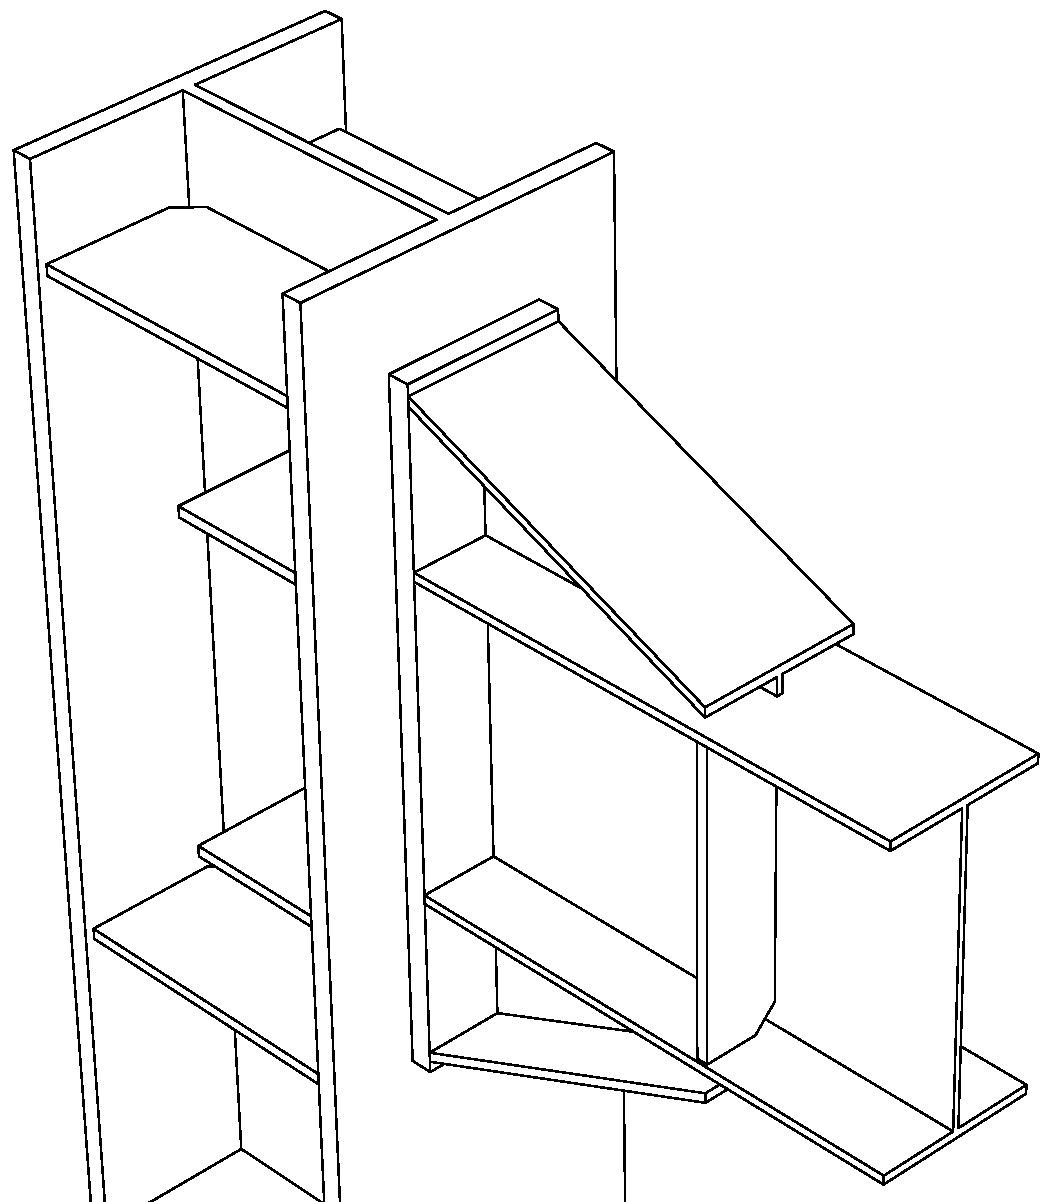
\includegraphics[width=.9\linewidth]{PIC/CH04/FR}
\caption{fully restrained}
\end{subfigure}\hfil
\begin{subfigure}{.5\linewidth}\centering
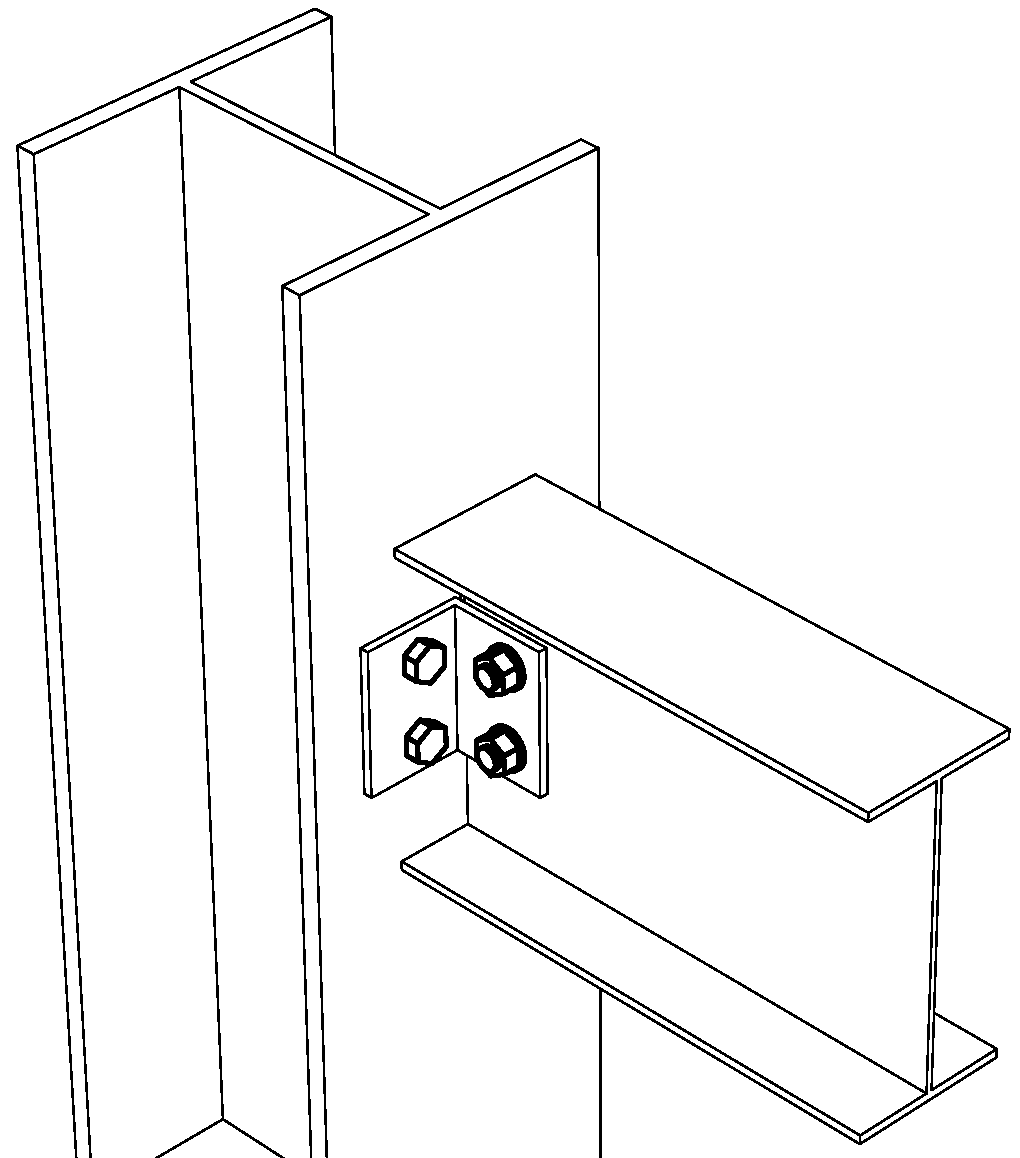
\includegraphics[width=.9\linewidth]{PIC/CH04/PR}
\caption{partially restrained}
\end{subfigure}
\caption{Connection types}
\end{figure}
\begin{figure}[H]
\centering\footnotesize
\begin{tikzpicture}[scale=.6]
\begin{scope}
\foreach\x in{0,4,8,12}
\draw[<-,thick](\x,5)--++(0,1);
\FixedSupport{0,0}{1.5}
\FixedSupport{4,0}{1.5}
\FixedSupport{8,0}{1.5}
\FixedSupport{12,0}{1.5}
\draw[line width=1mm](0,0)--++(0,4)--++(12,0)--++(0,-4)node[joint,fill=cc0066]{}(4,0)--++(0,4)(8,0)node[joint,fill=cc0066]{}--++(0,4);
\node[joint,fill=cc0066]at(4.2,4){};
\node[joint,fill=cc0066]at(7.8,4){};
\node[joint,fill=cc0066]at(8.2,4){};
\node[joint,fill=cc0066]at(11.8,4){};
\node[align=center]at(10,-2){PR\\leaning column\\connections};
\node[align=center]at(2,-2){FR\\connections};
\end{scope}
\begin{scope}[yshift=-10cm]
\foreach\x in{0,4,8,12}
\draw[<-,thick](\x+.4,5)--++(0,1);
\FixedSupport{0,0}{1.5}
\FixedSupport{4,0}{1.5}
\FixedSupport{8,0}{1.5}
\FixedSupport{12,0}{1.5}
\draw[line width=1mm](0,0)to[out=90,in=-90](0.4,4)--++(12,0)to(12,0)node[joint,fill=cc0066]{}(4,0)to[out=90,in=-90](4.4,4)(8,0)node[joint,fill=cc0066]{}--(8.4,4);
\node[joint,fill=cc0066]at(4.6,4){};
\node[joint,fill=cc0066]at(8.2,4){};
\node[joint,fill=cc0066]at(8.6,4){};
\node[joint,fill=cc0066]at(12.2,4){};
\node[align=center]at(10,-2){destabilizing\\effect};
\node[align=center]at(2,-2){stabilizing\\effect};
\end{scope}
\begin{scope}[xshift=15cm,yshift=-4cm]
\draw(0,0)rectangle(9,6);
\node[joint,fill=cc0066]at(0,0){};
\node[joint,fill=cc0066]at(0,6){};
\node[joint,fill=cc0066]at(9,6){};
\node[joint,fill=cc0066]at(9,0){};
\node[joint,fill=cc0066]at(3,2){};
\node[joint,fill=cc0066]at(3,4){};
\node[joint,fill=cc0066]at(6,2){};
\node[joint,fill=cc0066]at(6,4){};
%
\draw[ultra thick](0,2)node[fill=black]{}--(0,4)node[fill=black]{};
\draw[ultra thick](9,2)node[fill=black]{}--(9,4)node[fill=black]{};
\draw[ultra thick](3,0)node[fill=black]{}--(6,0)node[fill=black]{};
\draw[ultra thick](3,6)node[fill=black]{}--(6,6)node[fill=black]{};
\node[anchor=west]at(2.5,-2){plan of building};
\draw(2.5,-3)node[fill=black]{}node[right=4mm,anchor=west]{FR columns};
\draw(2.5,-4)node[joint,fill=cc0066]{}node[right=4mm,anchor=west]{PR (leaning) columns};
\end{scope}
\end{tikzpicture}
\caption{Destabilizaing effect of leaning columns}
\end{figure}
The FR frame provides a stabilizing effect for all of the columns, \NZSSTEEL{} requires that destabilizing effect of `leaning columns' be accounted for. For `leaning columns', use $k_e=1$.
\begin{exmp}\href{run:./WORKSHEET/CH04/EX4.ACLC.sm}{Worksheet}
Use Grade 300 steel. For the following sway frame, assume axial rigidity and out-of-plane buckling restrained. Design columns using UC sections.
\begin{figure}[H]
\footnotesize
\begin{tikzpicture}[scale=.4]
\begin{scope}
\FixedSupport{0,0}{1.5}{2}
\FixedSupport{10,0}{1.5}{2}
\FixedSupport{20,0}{1.5}{2}
\FixedSupport{30,0}{1.5}{2}
\draw[line width=1mm](0,0)node[joint,fill=exmpbg]{}--++(0,5)--++(10,0)--++(10,0)--++(10,0)--++(0,-5)node[joint,fill=exmpbg]{}(10,0)node[joint,fill=exmpbg]{}--++(0,5)(20,0)node[joint,fill=exmpbg]{}--++(0,5);
\node at(9.5,5)[joint,fill=exmpbg]{};
\node at(10.5,5)[joint,fill=exmpbg]{};
\node at(19.5,5)[joint,fill=exmpbg]{};
\node at(20.5,5)[joint,fill=exmpbg]{};
\draw[|<->|](0,-2)--++(10,0)node[midway,fill=exmpbg]{\SI{10}{\meter}};
\draw[|<->|](10,-2)--++(10,0)node[midway,fill=exmpbg]{\SI{10}{\meter}};
\draw[|<->|](20,-2)--++(10,0)node[midway,fill=exmpbg]{\SI{10}{\meter}};
\draw[|<->|](-2,0)--++(0,5)node[midway,fill=exmpbg]{\SI{5}{\meter}};
\setstructmech{convention=direction}
\NodalForce{0,9}[N][-\SI{1500}{\kn}][N][2]
\NodalForce{10,9}[N][-\SI{1900}{\kn}][N][2]
\NodalForce{20,9}[N][-\SI{1900}{\kn}][N][2]
\NodalForce{30,9}[N][-\SI{1500}{\kn}][N][2]
\node at(5,4){610UB101};
\node at(15,4){610UB101};
\node at(25,4){610UB101};
\end{scope}
\end{tikzpicture}
\end{figure}
\end{exmp}
\begin{solution}
For exterior columns, the total force to be carried is
\begin{gather*}
\sum{}N^*=2\times\left(\SI{1500}{\kn}+\SI{1900}{\kn}\right)=\SI{6800}{\kn}.
\end{gather*}
Try 310UC158, $f_y=\SI{280}{\mpa}$ and $r_x=\SI{139}{\mm}$,
\begin{gather*}
\gamma_{top}=\gamma_1=\dfrac{I_c/L_c}{\beta_eI_b/L_b}=\dfrac{\SI{388e6}{\mm^6}/\SI{5}{\meter}}{0.5\times\SI{761e6}{\mm^6}/\SI{10}{\meter}}=2.039,\\
\gamma_{bot}=\gamma_2=10.
\end{gather*}
Note the far end of the beam is pinned and sway is allowed, from \tabref{tab:beta_e}, $\beta_e=0.5$. From French equation, $k_e=2.126$. Thus,
\begin{gather*}
\lambda_n=\dfrac{k_eL}{r_x}\sqrt{k_f}\sqrt{\dfrac{f_y}{\SI{250}{\mpa}}}=\dfrac{2.126\times\SI{5}{\meter}}{\SI{139}{\mm}}\times\sqrt{1}\times\sqrt{\dfrac{280}{250}}=80.92.
\end{gather*}
This leads to $\alpha_c=0.674$,
\begin{gather*}
\phi{}N_c=\phi\alpha_ck_fA_nf_y=0.9\times0.674\times1\times\SI{20100}{\mm^2}\times\SI{280}{\mpa}=\SI{3415}{\kn}.
\end{gather*}
Thus, the total capacity of two columns is
\begin{gather*}
\sum\phi{}N_c=2\times\SI{3415}{\kn}=\SI{6830}{\kn}>\SI{6800}{\kn}.
\end{gather*}
For interior leaning columns, assume $f_y=\SI{280}{\mpa}$, try $r_x=\SI{100}{\mm}$,
\begin{gather*}
\lambda_n=\dfrac{k_eL}{r_x}\sqrt{k_f}\sqrt{\dfrac{f_y}{\SI{250}{\mpa}}}=\dfrac{1\times\SI{5}{\meter}}{\SI{100}{\mm}}\times\sqrt{1}\times\sqrt{\dfrac{280}{250}}=52.92.
\end{gather*}
Thus $\alpha_c=0.846$,
\begin{gather*}
A_n\geqslant\dfrac{N^*}{\phi\alpha_ck_ff_y}=\dfrac{\SI{1900}{\kn}}{0.9\times0.846\times1\times\SI{280}{\mpa}}=\SI{8909}{\mm^2}.
\end{gather*}
Thus choose 250UC72.9 for interior columns. It can be checked 250UC72.9 satisfies the design criterion by updating all quantities while the next designation 200UC59.5 does not. The braced capacity is greater than the sway capacity.

In conclusion, choose 250UC72.9 for interior columns and 310UC158 for exterior columns.
\end{solution}
\begin{exmp}Loading Dock

A loading dock is supported by four columns. It is braced in one direction and unbraced in the other. Find the column strength for different combinations of beam (310UB46.2 and 610UB125) and column (250UC89.5 and 310UC158) sections. The columns are oriented so that the weak axis direction is braced.
\begin{figure}[H]
\footnotesize
\begin{tikzpicture}[scale=.4]
\begin{scope}
\draw[line width=1mm,line join=round](0,0)coordinate(A)--++(0,6)coordinate(B)--++(8,0)coordinate(C)--++(0,-6)coordinate(D);
\draw[line width=1mm,line join=round](B)--++(30:6)coordinate(F)--++(0,-6)coordinate(E);
\draw[line width=1mm,line join=round](C)--++(30:6)coordinate(G)--++(0,-6)coordinate(H);
\draw[|<->|](0,-2)--++(8,0)node[midway,fill=exmpbg]{\SI{6}{\meter}};
\draw[|<->|](-2,0)--++(0,6)node[midway,fill=exmpbg]{\SI{4.5}{\meter}};
\draw[line width=1mm,line join=round](G)--(F);
\draw[line width=.4mm,line join=round](A)--(F)(B)--(E)(C)--(H)(D)--(G);
\FixedSupport{A}{1.5}{3}
\FixedSupport{D}{1.5}{3}
\FixedSupport{E}{1.5}{3}
\FixedSupport{H}{1.5}{3}
\node[joint,fill=exmpbg]at(A){};
\node[joint,fill=exmpbg]at(D){};
\node[joint,fill=exmpbg]at(E){};
\node[joint,fill=exmpbg]at(H){};
\draw[|<->|](10,-1)--++(30:6)node[midway,fill=exmpbg]{\SI{6}{\meter}};
\end{scope}
\end{tikzpicture}
\end{figure}
\end{exmp}
\begin{solution}
For all cases, $\beta_e=1$. Using the French equations, the effective lengths for each combination can be found as follows.
\begin{table}[H]
\centering\footnotesize
\renewcommand{\arraystretch}{1.2}
\begin{tabular}{ccccccc}
	\toprule
	  beam    &  column   &                        & $\gamma_{bot}$ & $\gamma_{top}$ & $k_e$ & $L_e$ \\ \midrule
	310UB46.2 & 250UC89.5 &   braced (weak axis)   &       10       &      0.65      & 0.83  & 3.75  \\
	          &           & unbraced (strong axis) &       10       &      1.91      & 2.10  & 9.45  \\
	310UB46.2 & 310UC158  &   braced (weak axis)   &       10       &      1.67      & 0.90  & 4.04  \\
	          &           & unbraced (strong axis) &       10       &      5.17      & 2.58  & 11.61 \\
	610UB125  & 250UC89.5 &   braced (weak axis)   &       10       &      0.07      & 0.71  & 3.21  \\
	          &           & unbraced (strong axis) &       10       &      0.19      & 1.70  & 7.67  \\
	610UB125  & 310UC158  &   braced (weak axis)   &       10       &      0.17      & 0.75  & 3.36  \\
	          &           & unbraced (strong axis) &       10       &      0.52      & 1.79  & 8.07  \\ \bottomrule
\end{tabular}
\end{table}
By looking up the design tables, the critical loads can be found.
\begin{table}[H]
\centering\footnotesize
\renewcommand{\arraystretch}{1.2}
\begin{tabular}{ccccccc}
	\toprule
	  beam    &  column   &  total weight  & braced capacity & unbraced capacity & critical &      load/weight      \\
	          &           & \si{\kilogram} &    \si{\kn}     &     \si{\kn}      & \si{\kn} & \si{\kn\per\kilogram} \\ \midrule
	310UB46.2 & 250UC89.5 &    2719.80     &     2310.07     &      1766.14      & 1766.14  &         2.60          \\
	310UB46.2 & 310UC158  &    3952.80     &     4254.20     &      3146.73      & 3146.73  &         3.18          \\
	610UB125  & 250UC89.5 &    4611.00     &     2441.89     &      2103.52      & 2103.52  &         1.82          \\
	610UB125  & 310UC158  &    5844.00     &     4472.80     &      4054.05      & 4054.05  &         2.77          \\ \bottomrule
\end{tabular}
\end{table}

Frame stiffness and therefore buckling capacity depend on stiffness of beams and columns. A proper combination shall be chosen to optimise the design (maximise load carried per weight).
\end{solution}
\subsection{Design of Columns in Frames}
In the previous discussion it is assumed that the columns are axially stiff.
\begin{itemize}
\item When columns are not axially stiff and loading is asymmetric, axial shortening occurs which leads to sidesway and moments.
\item When frame is not symmetric and columns are not axially stiff, sidesway and moments would be induced.
\item When member loads and lateral forces are present, moments develop in members.
\end{itemize}
\begin{figure}[H]
\centering\begin{tikzpicture}
\HingeSupport{0,0}
\HingeSupport{4,0}
\draw[dashed](0,0)|-(4,3)--(4,0);
\draw[<-,thick](0,3.5)--++(0,1)node[fill=white]{$P_1$};
\draw[<-,thick](4,3.5)--++(0,1)node[fill=white]{$P_2$};
\draw[line width=1.2mm](0,0)node[joint]{}to[out=92,in=-94](0-.1,3-.1)to[out=-4,in=190](4-.1,3-.2)to[out=-80,in=85](4,0)node[joint]{};
\begin{scope}[xshift=8cm]
\HingeSupport{0,0}
\HingeSupport{4,-1}
\draw[dashed](0,0)|-(4,3)--(4,-1);
\draw[<-,thick](0,3.5)--++(0,1)node[fill=white]{$P_1$};
\draw[<-,thick](4,3.5)--++(0,1)node[fill=white]{$P_2$};
\draw[line width=1.2mm](0,0)node[joint]{}to[out=95,in=-100](0-.2,3-.1)to[out=-10,in=170](4-.2,3-.3)to[out=-100,in=95](4,-1)node[joint]{};
\end{scope}
\end{tikzpicture}
\caption{Sidesway due to non-rigid columns}
\centering\begin{tikzpicture}
\HingeSupport{0,0}
\HingeSupport{4,0}
\draw[<-,thick](2,3.5)--++(0,1)node[fill=white]{$P_1$};
\setstructmech{showvalue=off,opacity=.5}
\IForceA[cc0066]{0,0}{0,3}{0}{-1}
\IForceA[cc0066]{0,3}{2,3}{1}{.5}
\IForceA[cc0066]{2,3}{4,3}{-.5}{-1}
\IForceA[cc0066]{4,0}{4,3}{0}{1}
\draw[line width=1.2mm](0,0)node[joint]{}|-(4,3)--(4,0)node[joint]{};
\begin{scope}[xshift=8cm]
\HingeSupport{0,0}
\HingeSupport{4,0}
\draw[<-,thick](-.5,3)--++(-1,0)node[fill=white]{$P_2$};
\IForceA[cc0066]{0,0}{0,3}{0}{1}
\IForceA[cc0066]{0,3}{4,3}{-1}{-1}
\IForceA[cc0066]{4,0}{4,3}{0}{1}
\draw[line width=1.2mm](0,0)node[joint]{}|-(4,3)--(4,0)node[joint]{};
\end{scope}
\end{tikzpicture}
\caption{Moment developed in columns due to horizontal loads}
\end{figure}
If moments occur in conjunction with axial force, then he member shall be designed for both moment and axial force. Furthermore, axial force will enhance moment ($P$-$\Delta$ and $P$-$\delta$ effects). We will discuss this in design of bending members.
\begin{sidewaysfigure}[p]
\centering\footnotesize
\begin{subfigure}{.5\linewidth}\centering
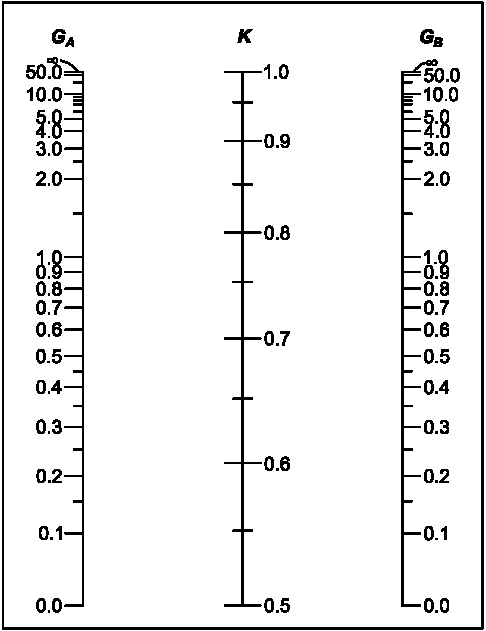
\includegraphics[width=.9\linewidth]{PIC/CH04/A360.BRACED}
\caption{alignment chart for $k_e$ for braced members}
\end{subfigure}\hfil
\begin{subfigure}{.5\linewidth}\centering
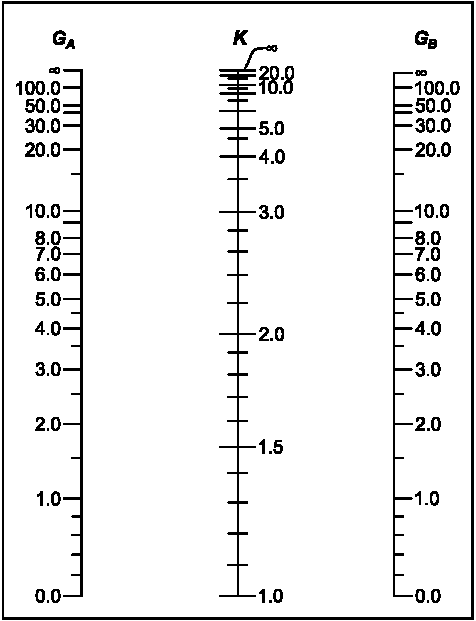
\includegraphics[width=.9\linewidth]{PIC/CH04/A360.SWAY}
\caption{alignment chart for $k_e$ for sway members}
\end{subfigure}
\end{sidewaysfigure}